\documentclass[a4paper,12pt]{article}
\usepackage[utf8]{inputenc}

%   Castellano
\usepackage[spanish,english,activeacute]{babel}
\decimalpoint
\usepackage{boxedminipage}

%   Matemáticas
\usepackage{ucs}
\usepackage{amsfonts}
\usepackage{amssymb}
\usepackage[T1]{fontenc}
\usepackage{amsmath}
\usepackage{lmodern}
\usepackage[margin=4cm]{geometry}
\usepackage{resizegather} %Para ecuaciones muy largas

%Import the natbib package and sets a bibliography  and citation styles
\usepackage{natbib}
\bibliographystyle{abbrvnat}
% \bibliographystyle{plain}
\setcitestyle{authoryear}
% \setcitestyle{authoryear,open={((},close={))}}
\usepackage{enumerate}
\usepackage{ftnxtra}

%footnote pegado a la zona inferior de la pagina
\usepackage[bottom]{footmisc}

%   Figuras
\usepackage{graphicx}
\DeclareGraphicsExtensions{.bmp,.pdf,.png,.jpg,.gif,.jpeg}
\usepackage[mathscr]{eucal}
\usepackage[nottoc]{tocbibind}
\usepackage[colorlinks,urlcolor=blue,citecolor=blue,linkcolor=blue,filecolor=blue]{hyperref}
\usepackage{subfig}

%   Tablas
%\usepackage{colortbl}% color
\usepackage{lscape}% vertical
% \usepackage{multirow}

% Tablas avanzadas
\usepackage{fancyhdr}
\markboth{izquierdo}{derecho}
\usepackage{pgfplotstable,array,booktabs}

%   Programación
\usepackage{minted}

\newmintedfile[mybash]{bash}{
    linenos,
    numbersep=4pt,
    gobble=0,
    frame=lines,
    framesep=2mm,
}

\newmintedfile[mypython]{python}{
    linenos,
    numbersep=5pt,
    gobble=0,
    frame=lines,
    framesep=2mm,
}

%Arbol directorios
\usepackage{tikz}
\usetikzlibrary{trees}

\usepackage{xcolor}
\tikzstyle{every node}=[thick,anchor=west, rounded corners, font={\scriptsize\ttfamily}, inner sep=2.5pt]
\tikzstyle{selected}=[draw=blue,fill=blue!10]
\tikzstyle{root}=[selected, fill=blue!30]

% Cambiar formato de una sola pagina
\usepackage{geometry}

%   Para introducir páginas en blanco
\usepackage{afterpage}

\usepackage[toc,page]{appendix}

%   formato del documento
%   Formato de las páginas
% altura cabecera
\setlength{\headheight}{1 pt}
% distancia cabecera caja
\setlength{\headsep}{20 pt}
% separación entre el pie y la caja
\setlength{\footskip}{10 mm}
% paperheight=margen superior, margen inferior 
\setlength{\textheight}{\dimexpr\paperheight-1.5 cm-\headheight-\headsep-\footskip-1 cm}
\setlength{\topmargin}{\dimexpr 1cm-1in}
% anchura pagina, margenes laterales
\setlength{\textwidth}{\dimexpr \paperwidth-1.75cm*2}
\setlength{\oddsidemargin}{\dimexpr 1.75cm-1in}

%   Comandos definidos por el usuario
%    NUEVOS COMANDOS DEFINIDOS MEDIANTE NEWCOMAND
\DeclareMathOperator\erf{erf}

% ENTORNO MATEMÁTICO
\newcommand{\maths}[1]{$ #1 $}

% TEXTO RESALTADO
\newcommand{\resalta}[1]{\textit{#1}}
\newcommand{\anglicismo}[1]{\textit{#1}}
\newcommand{\cultismo}[1]{\textit{#1}}
\newcommand{\comillas}[1]{``#1''}

% SÍMBOLOS MATEMÁTICOS
\newcommand{\menoroigual}{$\geqslant$}
\newcommand{\delorden}{$\sim$}
\newcommand\norm[1]{\left\lVert#1\right\rVert}
\newcommand{\porcentaje}[1]{$#1\:\%$}

%\lesssim  	less or quivalent
% \gtrsim 

% UNIDADES
%   PROPIAS DE ASTRONOMÍA
\newcommand{\solares}[2]{$#2 \:{#1}_{\odot}$}
\newcommand{\masassolares}[1]{$#1 \:{M}_{\odot}$}
\newcommand{\luminosidadessolares}[1]{$#1 \:{L}_{\odot}$}
\newcommand{\tfe}[1]{$#1 \:{M}_{\odot}\,\mathrm{{yr}^{-1}}$}
% \newcommand{\myr}{}
\newcommand{\flujo}[1]{${S}_{#1 \:\mu\mathrm{m}}$}
%   GENERALES
\newcommand{\microm}[1]{$#1 \:\mu\mathrm{m}$}
\newcommand{\angstrom}[1]{$#1 \:$\AA}
\newcommand{\mjy}[1]{$#1 \:\mathrm{mJy}$}
\newcommand{\jy}[1]{$#1 \:\mathrm{Jy}$}
\newcommand{\kelvin}[1]{$#1 \:\mathrm{K}$}
%   Grados celsius
\newcommand{\celsius}{\hspace{-2,5mm}$\phantom{a}^{\circ} \mathrm{C}$~}
\newcommand{\grad}{$^{\circ}$}

% NOMBRES USADOS FRECUENTEMENTE
\newcommand{\hatlas}{\mbox{\textit{H}-ATLAS}}
\newcommand{\halos}{\mbox{HALOS}}
\newcommand{\halo}{\mbox{HALO}}
\newcommand{\gama}{\mbox{GAMA}}
\newcommand{\spire}{\mbox{SPIRE}}
\newcommand{\pacs}{\mbox{PACS}}
\newcommand{\hifi}{\mbox{HIFI}}
\newcommand{\h}{\textit{\mbox{Herschel}}}
\newcommand{\rt}{\textit{\mbox{redshift}}}
\newcommand{\rts}{\textit{\mbox{redshifts}}}
\newcommand{\sed}{\mbox{SED}}
\newcommand{\sfr}{\mbox{SFR}}
\newcommand{\slg}{\mbox{SLG}}
\newcommand{\etg}{\mbox{ETG}}
\newcommand{\cross}{\mbox{cross-identificación}}
\newcommand{\smm}{\mbox{SMM~J2135-0102}}
\newcommand{\arp}{\mbox{Arp220}}
\newcommand{\gquince}{\mbox{G15.141}}

\newcommand{\typewriter}[1]{\texttt{#1}}
\newcommand{\python}{\texttt{\mbox{Python}}}

% PARÁMETROS
\newcommand{\z}{\textit{z}}
\newcommand{\paramk}{'K'}
\newcommand{\paramc}{'C'}

%   Compuestos químicos
\newcommand{\agua}{H_{2}O}

%   Nuevos comandos para tablas
%http://tex.stackexchange.com/questions/12703/how-to-create-fixed-width-table-columns-with-text-raggedright-centered-raggedlef
\newcolumntype{L}[1]{>{\raggedright\let\newline\\\arraybackslash\hspace{0pt}}m{#1}}
\newcolumntype{C}[1]{>{\centering\let\newline\\\arraybackslash\hspace{0pt}}m{#1}}
\newcolumntype{R}[1]{>{\raggedleft\let\newline\\\arraybackslash\hspace{0pt}}m{#1}}

%   Modificación de la linea para el pie de página
%https://es.wikibooks.org/wiki/Manual_de_LaTeX/Gestionando_la_bibliograf%C3%ADa/Notas_al_pie
\renewcommand{\footnoterule}{\vspace*{-3pt}
  \noindent\rule{5cm}{1pt}\vspace*{2.6pt}}
  
  
  
  

\newtheorem{theorem}{Teorema}[section]
\newtheorem{corollary}{Corollary}[theorem]
\newtheorem{lemma}[theorem]{Lemma}
\newtheorem{definition}{Definición}[section]

\renewcommand{\appendixname}{Anexos}
\renewcommand{\appendixtocname}{Anexos}
\renewcommand{\appendixpagename}{Anexos}

\usepackage{pgfplots}
\pgfplotsset{compat=1.15}

\begin{document}

\begin{titlepage}

    \begin{center}
    \vspace*{0.5in}
    
    \begin{figure}[htb]
        \begin{center}
            
\includegraphics[width=4cm]{00_Portada/UC.png}
        \end{center}
    \end{figure}
    
    \begin{Large}
        FACULTAD\\
        DE\\
        CIENCIAS\\
    \end{Large}
    
    \vspace*{0.6in}
    
    \begin{Large}
        \textbf{Selección de fuentes extragalácticas a alto redshift mediante una herramienta estadística de cross-identificación de catálogos de galaxias.} \\
    \end{Large}
    
    \vspace*{0.3in}
    
    \begin{large}
        (Selection of extragalactic sources at high redshift using a statistical tool for cross-identification of galaxy catalogs.)\\
    \end{large}
    
    \vspace*{0.3in}
    
    Trabajo de Fin de Grado\\
    para acceder al \\
    
    \vspace*{0.3in}
    
    GRADO EN FÍSICA
    
    \vspace*{1in}
    \end{center}

    \begin{flushright}
        \begin{large}
         Autor: Javier Gutiérrez Solórzano \\
         \vspace*{0.08in}
         Director: Diego Herranz Muñoz \\
         \vspace*{0.25in}
         Febrero, 2018
        \end{large}
    \end{flushright}

\end{titlepage}

\newpage
$\ $
\thispagestyle{empty} % para que no se numere esta pagina

\selectlanguage{spanish}

\section*{Agradecimientos}\label{sec:9_agradecimientos}

Quiero agradecer a mi director de proyecto, Diego Herranz su dedicación y disponibilidad para solucionar muchos de los problemas que han ido surgiendo durante el largo tiempo que ha supuesto la elaboración de este trabajo. Extiendo mi agradecimiento a Joaquín González-Nuevo porque su ayuda ha sido imprescindible para implementar correctamente el método para la estimación del desplazamiento al rojo de las galaxias submilimétricas.

También quiero mostrar mi especial gratitud a mis padres por todo el tiempo que ellos invierten para que yo pueda hacer esto y muchas otras cosas más.

\newpage
$\ $
\thispagestyle{empty}

%   Tabla de contenidos
\addcontentsline{toc}{section}{Resumen}
\tableofcontents



\selectlanguage{spanish}

\begin{abstract}
Se ha propuesto un método para la búsqueda de galaxias en fases tempranas de su formación suponiendo que la imagen observada ha sido magnificada por el efecto de una lente gravitatoria. 
El método consiste en seleccionar un subconjunto de emparejados que surgen al aplicar un criterio estadístico de \cross\ basado en el factor de Bayes a los catálogos \hatlas\ DR1 y \gama\ DR1. El factor de Bayes utilizado consta de un término basado en la separación angular entre entre dos observaciones y otro basado en el corrimiento al rojo. En los casos en los que se cuenta con una medida fiable del corrimiento al rojo de la fuente perteneciente a \hatlas,\hspace{1mm} se utilizarán esos valores. En caso de que no se disponga, se obtendrá su \rt\ fotométrico a partir de un ajuste por mínimos cuadrados de la distribución espectral de energía de una galaxia modelo a tres medias del flujo espectral de la fuente a tres longitudes de onda concretas. Si el factor de Bayes da una alta probabilidad de que el par de observaciones no pertenecen a un mismo objeto, pero el término que depende de la distancia angular sugiere que si lo son, entonces tenemos un buen candidato para ser una lente gravitatoria.

El método desarrollado para estimar el corrimiento al rojo ha dado buenos resultados al compáralo con trabajos anteriores. Por su parte los resultados obtenidos mediante el método bayesiano para la identificación de lentes muestra una pureza relativamente baja pero resulta prometedor como fase previa a un estudio más detallado porque permite identificar de una forma rápida, sencilla y directa, basada en un criterio estadístico riguroso, entorno al tres por ciento de los candidatos con mayor probabilidad de ser sistemas lente de entre las galaxias del catálogo \hatlas\ DR1.

\end{abstract}


\textbf{Palabras clave:} Alto desplazamiento al rojo -- galaxias submilimétricas -- lente gravitatoria fuerte -- factor de Bayes -- \mbox{cross-identificación}


\selectlanguage{english}

\begin{abstract}
A method has been proposed for the search of galaxies in early phases of their formation supposing that the observed image has been magnified by the effect of a gravitational lens. The method consists of selecting a subset of paired that arise by applying a statistical criterion of cross-identification based on the Bayes factor to the catalogs \hatlas\ DR1 and \gama\ DR1. The Bayes factor used consists of a term based on the angular separation between two observations and another based on the redshift. In those cases in which a reliable measure of the redshift of the source belonging to \hatlas\ is available, these values will be used. If it is not available, its photometric redshift will be obtained from a least squares fit of the spectral energy distribution of a model galaxy to three measures of the spectral flux of the source at three specific wavelengths. If the Bayes factor gives a high probability that the pair of observations do not belong to the same object, but the term that depends on the angular distance suggests that if they are, then we have a good candidate to be a gravitational lens.

The method developed to estimate the redshift has given good results when compared to previous works. On the other hand, the results obtained by the Bayesian method for the identification of lenses show a relatively low purity but it is promising as a previous phase to a more detailed study because it allows to identify in a fast, simple and direct way, based on a rigorous statistical criterion, around the three percent of the candidates most likely to be lens systems among the galaxies in the \hatlas\ DR1 catalog.

\end{abstract}


\textbf{Key words:} high-redshift -- submillimiter galaxies -- strong gravitational lensing -- Bayes factors -- \mbox{cross-identification}


\newpage
$\ $
\thispagestyle{empty}

\selectlanguage{spanish}

\section{Introducción}\label{sec:1_introduccion}

Los objetos con alto desplazamiento al rojo o alto \rt \footnote{A lo largo del trabajo haremos referencia a objetos con un \rt\ alto, medio y bajo. La distinción típica que se encuentra en la literatura es: alto \rt\ \maths{z>1}, \rt\ intermedio \maths{0.1<z<1} y \rt\ bajo \maths{z<0.1}} en inglés, (en lo sucesivo utilizaremos el término \rt\ por brevedad) son muy importantes para entender cómo se formaron las estructuras que observamos en el universo actual. En su gran mayoría se trata de galaxias en estadios tempranos de su formación que se caracterizan por una magnitud aparente muy débil y una emisión electromagnética principalmente en la zona infrarroja (IR) del espectro. Debido a que la generación actual de telescopios infrarrojos (en especial aquellos que operan en el infrarrojo lejano, \microm{\lambda\sim100-500}) tienen una resolución espacial bastante limitada en comparación con los telescopios ópticos (la resolución angular de un telescopio con apertura circular es proporcional al inverso de su diámetro y los telescopios que operan en el \mbox{IR-lejano} deben ser telescopios espaciales pues la atmósfera es opaca en esa zona del espectro) las medidas realizadas sobre las galaxias tempranas en formación\footnote{También nos referiremos a estos objetos como \comillas{galaxias lejanas}, \comillas{galaxias submilimétricas} (en referencia al rango del espectro en el que son mas brillantes), o \comillas{galaxias tempranas}. Debe quedar claro que en este trabajo cuando utilizamos el término \comillas{galaxia temprana} nos referimos siempre a un orden cronológico y no a la morfología de la galaxia.} (\mbox{ETGs}) tienen una gran contaminación debido a la presencia de otras fuentes débiles en sus proximidades y son especialmente difíciles de estudiar. 

A veces, la luz procedente de los objetos lejanos resulta desviada debido a la presencia de objetos muy masivos que se interponen entre estas fuentes y nosotros (generalmente galaxias elípticas y grupos de galaxias) y se producen intensas magnificaciones (entendiéndose como un incremento sobre el brillo original) de la imagen del objeto fuente. Este fenómeno, conocido como lente gravitatoria, lejos de ser un problema está resultando ser una importante herramienta para el estudio de las propiedades individuales y estadísticas de las galaxias submilimétricas~(SMGs). Eso ha motivado la aparición de distintas propuestas para la identificación de galaxias lejanas lensadas\footnote{En las publicaciones realizadas en lengua inglesa, se refieren a estos objetos con el nombre de \comillas{\anglicismo{gravitationally lensed galaxies}}, sin embargo resulta difícil traducir correctamente esta terminología al castellano. A falta de una traducción mejor usaremos la palabra \comillas{lensar} en lugar del término \anglicismo{lensed}.} (SLGs) entre los cartografiados de galaxias actuales. En particular, los trabajos de \cite{article:Negrello_2010} y \cite{article:Nuevo_2012} proponen unos criterios para seleccionar este tipo de galaxias a partir de las medidas del telescopio espacial infrarrojo \h. Ambos criterios proponen la identificación de los candidatos a partir de la selección de distintos flujos de corte para un conjunto de frecuencias consideradas. Estos métodos, como cualquier otro, tienen sus propios sesgos de selección, por lo que resultaría interesante disponer de otros métodos radicalmente diferentes para seleccionar SLGs.

En este trabajo planteamos la búsqueda de SLGs  identificando sistemas lente gravitatoria completos, es decir, encontrando no solo el objeto fuente que ha sido lensado, sino también el objeto lente cuya masa es responsable de la desviación de la luz procedente de la fuente. Al igual que los autores anteriores, nosotros proponemos la búsqueda de SLGs en el catálogo \hatlas\ porque es sensible a las longitudes de onda en el IR-lejano en el que se produce el máximo de emisión de las ETGs y porque se ha estimado que la sección eficaz de detección de lentes a alto \rt\ por el instrumento \spire\ es muy favorable \citep{article:Negrello_2010}. En este caso, debido a que existe una zona de solapamiento entre los cartografiados \hatlas\ y \gama\ y también debido a que la distribución en \rt\ de los objetos del catálogo \gama\ es la adecuada, consideramos el catálogo \gama\ como una buena elección para encontrar en él los objetos lente. Nuestra idea consiste en aplicar un criterio estadístico de \cross\ de catálogos de galaxias para identificar lentes gravitatorias en las que participa como objeto fuente una \etg. El método consta de dos factores de Bayes propuestos por \cite{article:Tamas_Budavari_2008} y  \cite{article:Tamas_Budavari_2011}; uno de ellos depende de la separación angular entre las observaciones\footnote{En este trabajo se entiende por observación al conjunto de dos medidas: posición y desplazamiento al rojo. Cada catálogo realiza sus propias observaciones de forma independiente.} y otro de la diferencia entre los \rt. Cada emparejado considerado está formado por dos observaciones, una de ellas perteneciente al catálogo \hatlas\ y la otra a \gama. En los casos en los que se cuenta con una medida fiable del corrimiento al rojo de la observación realizada por \hatlas\ se utilizarán esos valores; en caso de que no se disponga de dicha información, se realizará un ajuste por mínimos cuadrados de la distribución espectral de energía (\sed) de una galaxia modelo a tres medidas del flujo espectral en tres longitudes de onda diferentes realizadas por el instrumento \spire. Si el ajuste se considera adecuado proporcionará el \rt\ fotométrico de la fuente. En el caso de que el factor de Bayes conjunto dé una alta probabilidad de que el par de observaciones no pertenezcan a un mismo objeto, pero el término que depende de la distancia angular sugiere que si lo son, el par de observaciones es considerado un sistema lente gravitatoria.

La memoria está dividida en varias secciones: la Sección \ref{sec:1_introduccion} contiene una explicación básica de algunos de los conceptos más importantes que serán usados a lo largo del trabajo; la Sección \ref{sec:2_muestras} pretende dar una explicación general de los catálogos utilizados y de los instrumentos con los que se realizaron; la Sección \ref{sec:3_redshift_hatlas} describe el método utilizado en este trabajo para calcular el \rt\ fotométrico de las ETGs a partir de las medidas del instrumento \spire, se explicarán también los fundamentos en los que se basa y confrontaremos el \rt\ obtenido para un conjunto de  galaxias con los obtenidos por otros autores; en la Sección \ref{sec:4_cross_identificacion} describiremos en detalle el método de \cross\ utilizado; en la Sección \ref{sec:5_halos} se describirán las distintas propuestas para para identificar los sistemas que conforman lentes gravitatorias, incluida la nuestra; en la Sección \ref{sec:6_resultados} se mostrarán\linebreak los resultados obtenidos y finalmente, Sección \ref{sec:7_conclusiones}, expondremos nuestras conclusiones. Los apéndices contienen tablas y el código de los programas escritos en lenguaje de programación \python.


\subsection{Galaxias con alto desplazamiento al rojo.}\label{subsec:galaxias_alto_rojo}

Las galaxias con alto desplazamiento al rojo son galaxias muy lejanas, cuya luz ha tardado miles de millones de años en recorrer la distancia que nos separa de ellas y que ahora, vistas desde la Tierra, muestran el aspecto que tuvieron cuando la luz partió de ellas. Estos objetos juegan un papel fundamental en cosmología, porque su estudio permite comprender cómo se formaron las galaxias actuales.
Una de las predicciones fundamentales de la teoría del \anglicismo{Big Bang} es que el universo temprano consistía en materia y radiación distribuida de forma homogénea y en equilibrio termodinámico. Hoy día el universo es altamente heterogéneo, formando estructuras como estrellas, galaxias, cúmulos y supercúmulos de galaxias. Entender cómo se produjo esta etapa de transición entre el universo homogéneo a la formación de las estructuras que se observan en el universo actual, es uno de los objetivos de la cosmología y de la física fundamental.

\subsubsection{Características de las galaxias con alto desplazamiento al rojo.}

Se especula que las primeras galaxias, se formaron a partir de nubes de gas compuestas por hidrógeno y pequeñas cantidades de helio y litio. En estas condiciones se formaron un gran número de estrellas, en un periodo de tiempo relativamente corto, conocido como \anglicismo{starburst} (estallido estelar). Para una galaxia del tamaño de la Vía Láctea con \maths{\sim {10}^{11}} estrellas, se cree que el proceso duró \maths{\sim {10}^8\;\mathrm{yr}}, lo que implica una tasa de formación estelar (SFR) \tfe{\sim 10^3}, una cifra enorme si se compara con la tasa de formación estelar actual de la misma \tfe{\sim 1} \citep{book:encyclopedia}. Estas primeras estrellas, forman la primera generación de estrellas en el Universo, llamada Población III y tenían unas características distintas a las actuales. Se cree que eran muy masivas, llegando a poseer masas de hasta \masassolares{100}. Actualmente, las nebulosas donde se forman las nuevas estrellas contienen metales\footnote{ Se entiende por metales todos los núcleos atómicos con masa atómica superior al He. Estos elementos no se encontraban en el universo antes de la aparición de las primera estrellas.}, lo cual incrementa su opacidad; la radiación emitida durante el colapso de la nebulosa interacciona con el material y parte de él no pasa a formar la estrella, porque que es expulsado, lo cuál limita la masa de las estrellas actuales. Las estrellas muy masivas queman muy rápidamente su combustible nuclear (los modelos indican que una estrella como el Sol está en la secuencia principal \maths{\sim {10}^{10}} años, mientras que las estrellas masivas con \masassolares{>25} tienen una vida media de menos de \maths{7\times{10}^{6}} años, \citealt{book:encyclopedia}), y finalizan su vida como supernovas que expulsan grandes cantidades de residuos nucleares que enriquecen el medio interestelar con elementos pesados.

Las estrellas pertenecientes a estas primera etapas del Universo debieron ser grandes emisoras de luz y radiación ultravioleta (UV). Las grandes nubes de gas y polvo que se encontraban en las galaxias que las albergaban absorbían una parte esta radiación y la remitían en el IR. Las temperaturas de equilibrio térmico para esas nubes se encuentran el rango de \maths{10-100\;\mathrm{K}}, lo que da lugar la emisión IR en la región \maths{\lambda \sim 30-300\;\mu \mathrm{m}} \citep{book:encyclopedia}.
Los halos galácticos de las galaxias espirales actuales de tipo S\maths{a} están compuestos por poblaciones de estrellas viejas, con edades \maths{\gtrsim 8-9\; \mathrm{Gyr}} (lo que corresponde a \maths{z\gtrsim 1-1.5}, \citealt{article:Lapi_2011}), las cuales se formaron a partir de los residuos nucleares de las estrellas que las precedieron y conforman la llamada Población II; por tanto, las ETGs muestran desplazamientos al rojo \maths{z \gtrsim 1}. La radiación IR procedente de una nube de polvo y gas interestelar perteneciente a una galaxia con un desplazamiento al rojo \maths{z=1} debería encontrarse en la zona del espectro con \maths{\lambda \sim 60-600\;\mu \mathrm{m}} (estas cifras se obtienen fácilmente a partir de la Ecuación \ref{eq:z_general} y el rango de emisión de las nubes al que se ha hecho referencia anteriormente). Estos datos suponen un punto de partida para la búsqueda de ETGs a partir de su observación en la zona IR del espectro.

\subsection{Desplazamiento al rojo.}

El desplazamiento al rojo (o desplazamiento al azul) es el desplazamiento del espectro electromagnético de un objeto hacia longitudes de onda mayores (o más cortas) que puede deberse a movimientos cinemáticos entre el emisor y el receptor (\maths{z_{mov}}, efecto Doppler), a efectos gravitatorios (\maths{z_{grav}}) o a la expansión de la métrica del universo a grandes escalas (\maths{z_{H}}). Dado un desplazamiento al rojo \maths{z}, podemos descomponerlo como la suma

\begin{equation}\label{eq:z_descomposicion}
    z= {z}_{mov}+{z}_{grav}+{z}_{H},
\end{equation}

de las distintas contribuciones citadas anteriormente. La definición general de corrimiento al rojo, siempre válida, independientemente de la causa que lo originó, es

\begin{equation}\label{eq:z_general}
    z=\frac{\lambda_o-\lambda_e}{\lambda_e}=\frac{\lambda_o}{\lambda_e}-1,
\end{equation}

donde los subíndices hacen referencia a la longitud de onda emitida \maths{e} y observada \maths{o}.

\subsubsection{Desplazamiento al rojo cosmológico.}

Cuando se habla de desplazamiento al rojo en el contexto de la cosmología, nos estamos refiriendo al hecho de que la distribución espectral de energía de las galaxias lejanas se encuentra desplazada hacia longitudes de onda mayores.  
Este hecho fue observado ya en el siglo XIX por aquellos que comenzaron a identificar líneas espectrales en los espectros emisión de los cuerpos celestes que en aquel momento se conocían como nebulosas\footnote{En aquel momento se conocían como nebulosas todos aquellos cuerpos celestes cuya luz no parecía provenir de una fuente puntual y su apariencia era similar a una nube de luz difusa. No estaba todavía establecida la diferencia entre nebulosas y galaxias.}.  Entre 1912 y 1925 el astrónomo italiano Vesto Sliper midió la posición de las líneas de emisión de unas 40 de estas nebulosas y constató por primer vez y para su sorpresa que, en todas ellas, las líneas se encontraban desplazadas hacia longitudes de onda inferiores con respecto a las mismas líneas espectrales medidas en el laboratorio \citep{book:cosmologia}. 
Posteriormente Edwin Hubble y su ayudante Milton Humanson, que disponían del mejor telescopio construido hasta entonces en el monte Palomar, Arizona, dieron un paso más en la comprensión del fenómeno. En primer lugar extendieron la lista elaborada por Sliper y probaron que en ningún caso el espectro se encontraba desplazado hacia el azul. En segundo lugar, Hubble identificó estrellas variables cefeidas en varios de estos cuerpos nebulosos\footnote{Fueron precisamente estudios como los que llevó a cabo Hubble para determinar las distancias, los que pusieron en evidencia que las galaxias y las nebulosas son objetos muy diferentes.} y gracias a ello pudo medir por primera vez la distancia a esos objetos. Interpretó el desplazamiento al rojo como un efecto Doppler y halló su velocidad a partir de la expresión

\vspace{-5mm}

\begin{equation}
    v\approx c z,
\end{equation}

e hizo una representación gráfica de la velocidad asociada a ese desplazamiento al rojo frente a la distancia que el midió. Se dio cuenta de que había una relación lineal entre la velocidad que y la distancia,

\begin{equation}
    v={H}_{0}D \implies z= ({H}_{0}/c)D.
\end{equation}

Ésta última igualdad es conocida como la ley de Hubble y \maths{{H}_0} como constante de Hubble.

\begin{figure}[htb]
    \begin{center}
         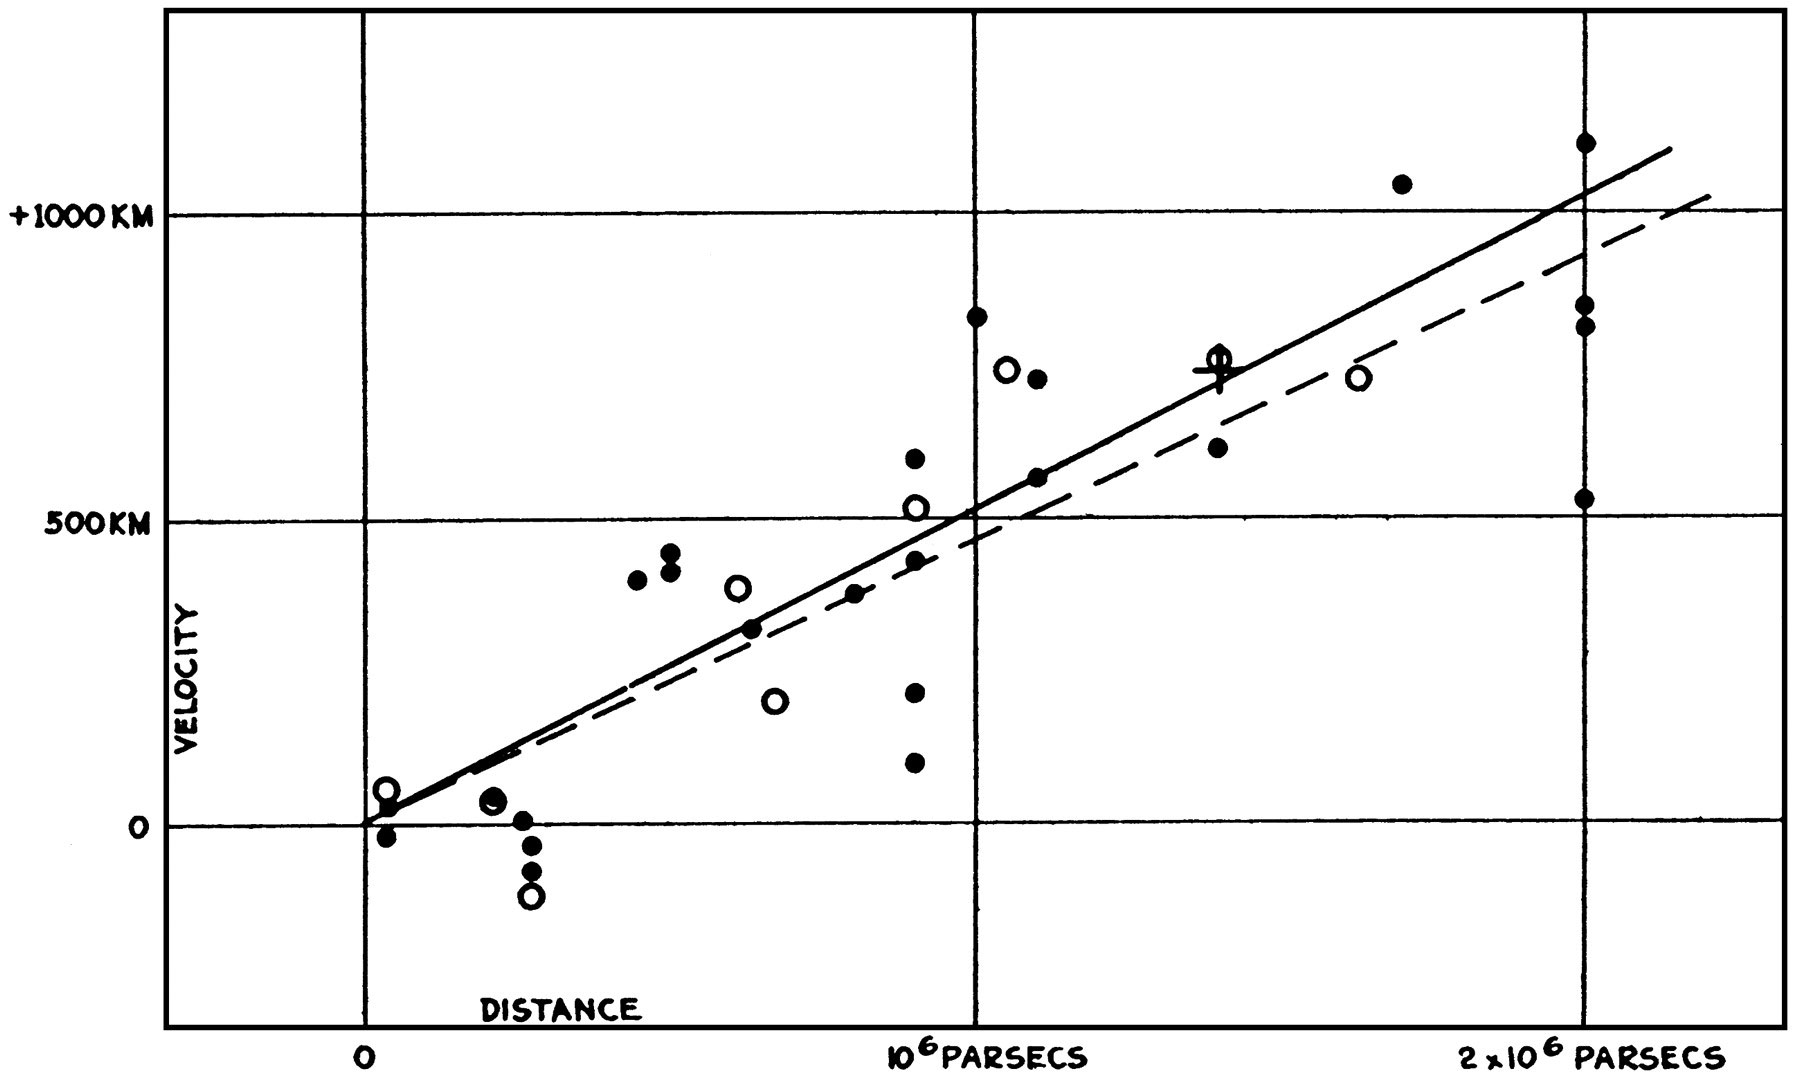
\includegraphics[width=13cm]{1_Introduccion/hubble.jpg}
    \end{center}
    
    \caption{\small Gráfica de una de las publicaciones originales de Hubble. Pone en evidencia que Hubble interpretó el desplazamiento al rojo como debido al efecto Doppler. \comillas{Una Relación entre la Distancia y Velocidad Radial en las Nebulosas Extra-Galácticas}, Los Procesos de la Academia Nacional de Las Ciencias, Volumen 15, Edición 13, 1929: p. 172. ©Huntington Library, San Marino, CA. Fuente: \url{https://www.visionlearning.com/es/library/Proceso-de-la-Ciencia/49/La-Naturaleza-del-Conocimiento-Cient\%c3\%adfico/185}}
    \label{fig:publicacion_hubble}
\end{figure}

Es conveniente aclarar dos puntos. En primer lugar la ley de Hubble no relaciona en realidad velocidades con distancias, sino desplazamientos al rojo con distancias. Esta confusión es debida a que inicialmente el desplazamiento al rojo se achacó a un efecto Doppler tal y como se deduce de las publicaciones originales de Hubble (Figura~\ref{fig:publicacion_hubble}). En segundo lugar, la ley de Hubble no es un modelo físico, es un hecho observable. Actualmente se ha medido del orden de \maths{{10}^{6}} desplazamientos y solo \maths{\sim10} de ellos muestran desplazamientos hacia el azul, siendo estos últimos, todos ellos, objetos del Grupo Local.
Por tanto cualquier interpretación de este fenómeno debe ser coherente con los siguientes puntos:

\vspace{-2mm}
\begin{itemize}
    \item El desplazamiento siempre se produce hacia longitudes de onda mayores, a excepción de los objetos que se encuentran en el Grupo Local.
    \vspace{-2mm}
    
    \item El desplazamiento no depende de la frecuencia, afecta a todo el espectro electromagnético de la misma forma.
    \vspace{-2mm}
    
    \item El desplazamiento es lineal con la distancia al objeto, al menos para el caso de los objetos más próximos, cuya distancia se ha podido determinar por métodos directos.
    \vspace{-2mm}
    
    \item Los desplazamientos son isótropos, es decir, no dependen de la dirección en la que se encuentren en la bóveda celeste, únicamente de la distancia que nos separa de los mismos.
    
\end{itemize}

Además se impone que todas las condiciones anteriores deben cumplirse en cualquier lugar del Universo. Es obvio que no hay evidencia experimental de que esto se cumpla; se trata de una suposición basada en lo que se conoce como principio anti-antropocéntrico, es decir, el observador no se encuentra en un lugar privilegiado. 
Actualmente, la explicación más ampliamente aceptada es la conocida como evolución de la métrica, por ser prácticamente la única explicación disponible. Esta explicación acepta que existe un factor de escala que cambia con el tiempo cosmológico, aumentando la distancia radial que nos separa de los objetos. Dado que la velocidad de la luz es finita y las distancias que nos separan incluso de las galaxias más próximas es enorme, los intervalos de tiempo que tarda la luz en alcanzarnos son lo suficientemente grandes como para que el factor de escala haya cambiado sensiblemente afectando a la longitud de onda de la radiación electromagnética mientras se transmite por el espacio\footnote{Es muy interesante observar que el factor de escala solo afecta al universo a grandes escalas como la distancia entre galaxias. Si el factor de escala afectase a escala de laboratorio de la misma forma que a las escalas astronómicas, cambiaría también nuestros patrones de medida incrementándose en la misma proporción y haciendo indetectable la expansión del universo.}. Los desplazamientos hacia el azul que se observan entre los objetos del Grupo Local se deben a que tienen un movimiento cinemático dirigido hacia nosotros y a que se encuentran relativamente próximos. En este caso, la contribución a $z$ debida al efecto Doppler resulta más importante que la debida a la expansión de la métrica, que siempre contribuye a un desplazamiento al rojo. Para objetos muy lejanos la expansión de la métrica resulta dominante siempre.

A continuación se muestra cómo afecta el cambio del factor de escala a las propiedades de la luz que viaja por el espacio, partiendo de la métrica utilizada en el modelo cosmológico estándar \citep{book:cosmologia}. En un universo en expansión, el \rt\ está directamente relacionado con la distancia.
En el modelo cosmológico estándar de Friedmann-Lema\^{i}tre, las distancias están definidas a partir de la métrica de Robertson-Walker\footnote{Se  demuestra en \cite{book:weinberg_1974} que es la métrica más general que describe un espacio de tetra-dimensional, con tres dimensiones espaciales y una temporal y cuyo subespacio espacial tiene curvatura arbitraria y es maximalmente simétrico.}

\begin{equation}\label{eq:metrica_RW}
    {\mathrm ds}^{2}= {c}^{2}\mathrm dt^2 +{R}^{2}(t) \left( \frac{{\mathrm dr}^{2}}{1-\kappa {r}^{2}} + {r}^{2}\mathrm d{\theta}^{2} +{r}^{2}{\sin}^{2}{\theta}\,\mathrm d{\varphi}^{2} \right),
\end{equation}

siendo \maths{R(t)} el factor de escala, \maths{\kappa} el signo de la curvatura que puede tomar los valores -1, 0 o 1, \textit{t} el tiempo cosmológico y \textit{r}, \maths{\theta} y \maths{\varphi} las coordenadas comóviles expresadas en un sistema de coordenadas esféricas. Debido a la isotropía del espacio, la distancia propia solo depende de la coordenada radial comóvil \maths{r} y es constante con \maths{\theta} y \maths{\varphi}, con lo cual, la métrica se simplifica reduciéndose a

\begin{equation*}
    {\mathrm ds}^{2}= {c}^{2}\mathrm dt^2 +{R}^{2}(t)\;\frac{{\mathrm dr}^{2}}{1-\kappa {r}^{2}}.
\end{equation*}

Supongamos que se emiten dos pulsos de luz. El primero se emite desde un punto coordenada radial comóvil \maths{r=r_e} y tiempo cosmológico \maths{t=t_e}. El segundo con las mismas coordenadas espaciales y un tiempo cosmológico \maths{t_e+T_e}. Estos pulsos se propagan por el espacio durante un tiempo suficientemente grande, como el tiempo necesario para cruzar el espacio entre dos galaxias próximas, tras el cual alcanzan a un observador. El primer pulso lo alcanza en coordenadas \maths{r=0} y \maths{t=t_o}, mientras que el segundo alcanza al observador en \maths{r=0} y \maths{=t_o+T_o}. Teniendo en cuenta que las ondas luminosas viajan por geodésicas (\maths{\mathrm{d}s=0}) y dado que los dos pulsos fueron emitidos y finalmente recibidos en puntos con las mismas coordenadas espaciales, tenemos que:

\begin{equation*}
    \int_{t_e}^{t_0} \frac{\mathrm d t }{R(t)}=\int_{t_e+T_e}^{t_o+T_o} \frac{\mathrm d t }{R(t)}=-{c}^{-1}\int_{r_e}^{0} \frac{\mathrm d r}{\sqrt{1-\kappa {r}^{2}}}.
\end{equation*}

Centraremos la atención en la igualdad establecida por las integrales en las que participa el factor de escala. En principio no podemos realizar las integrales porque desconocemos la función \maths{R(t)}; sin embargo podemos realizar una manipulación sobre los limites de integración:

\begin{align*}
    \int_{t_e+T_e}^{t_o+T_o} \frac{\mathrm d t }{R(t)} =\int_{t_e}^{t_0} \frac{\mathrm d t }{R(t)}\equiv \int_{t_e}^{t_e+ T_e} \frac{\mathrm d t }{R(t)} + \int_{t_e+T_e}^{t_o} \frac{\mathrm d t }{R(t)} \implies \nonumber\\
    \int_{t_e}^{t_e+T_e} \frac{\mathrm d t }{R(t)}= \int_{t_o}^{t_e+ T_e} \frac{\mathrm d t }{R(t)} + \int_{t_e+T_e}^{t_o+T_o} \frac{\mathrm d t }{R(t)} \equiv  \int_{t_o}^{t_o+T_o} \frac{\mathrm d t }{R(t)}. \nonumber \\
\end{align*}

De esta forma, si los tiempos de integración \maths{T_e} y \maths{T_o} han sido mucho más pequeños que el tiempo de propagación de los pulsos por el espacio, el factor de escala puede considerarse constante, teniendo distintos valores cuando los pulsos fueron emitidos y cuando fueron recibidos:

\begin{equation*}
    \frac{1}{R(t_e)}\int_{t_e}^{t_e+T_e} \mathrm d t = \frac{1}{R(t_o)} \int_{t_o}^{t_o + T_o} \mathrm d t \implies \frac{T_e}{R(t_e)}=\frac{T_o}{R(t_o)}.
\end{equation*}

Por comodidad podemos considerar que \maths{T_e} y \maths{T_o} son los periodos de la onda luminosa cuando fue emitida y cuando fue observada, respectivamente. Utilizando la ecuación \maths{T=\lambda/c} y la definición general de corrimiento al rojo (Ec. \ref{eq:z_general}) obtenemos que

\begin{equation}\label{eq:metrica_vs_z}
    \frac{R(t_o)}{R(t_e)}=\frac{\lambda_o}{\lambda_e}=1+z.
\end{equation}

El desplazamiento al rojo no se debe por tanto a un efecto Doppler, si no porque el incremento del factor de escala, afecta de la misma forma a la longitud de onda de la radiación electromagnética durante el tiempo de propagación que a las distancias propias.

Desarrollando en serie de Taylor el inverso del factor de escala en torno a \maths{t=t_o},

\begin{align}
    z =\frac{R(t_o)}{R(t_e)}-1 & = \frac{\dot{R}(t_o)}{R(t_o)}(t_o-t)+\left[ {\left(\frac{\dot{R}(t_o)}{R(t_o)}\right)}^{2}-\frac{1}{2}\frac{\ddot{R}(t_o)}{R(t_o)}\right]{(t_o-t)}^{2} +\cdots \nonumber
\end{align}

podemos recuperar la ley de Hubble al identificar el término \maths{\dot{R}(t_o)/R(t_o)} con el valor de la  constante de Hubble en el tiempo cosmológico actual \maths{H_o} y truncándolo en el término de segundo orden

\vspace{-3mm}
 
\begin{align}
    z={H}_{o}(t_o-t)+{H}_{o}^{2}\left[1+\frac{1}{2} {q}_{o} \right]{(t_o-t)}^{2} +\cdots .\nonumber
\end{align}

La ley de Hubble en el contexto del modelo estándar debe considerarse como una aproximación a la Ecuación \ref{eq:metrica_vs_z} \citep{book:cosmologia}.

\subsection{Técnicas para determinar el desplazamiento al rojo.}

En este trabajo estaremos haciendo referencia continuamente a \comillas{\rt\ espectroscópicos} y \comillas{\rt\ fotométricos}. Esos nombres hacen referencia a la técnica con la que se obtuvo esa medida. A continuación se explicará brevemente en que consisten estas técnicas. Cabe mencionar que el método propuesto en la Sección \ref{sec:3_redshift_hatlas} de esta memoria forma parte de las técnicas fotométricas.

\subsubsection{\anglicismo{Redshift} espectroscópico.}

Cuando se habla de \rt\ espectroscópico nos estamos refiriendo a una técnica para determinar el \rt\ de los objetos celestes. El \rt\ espectroscópico consiste en identificar algunas de las líneas espectrales de absorción o emisión de algún elemento químico en la luz proveniente de un objeto celeste y comparar la longitud de onda a la que se encuentran con la que debería tener si proviniesen de una muestra en reposo. Este es el primer método que se utilizó para determinar el desplazamiento al rojo de los objetos celestes y permite determinar el \rt\ de forma muy precisa; el problema que tiene es que requiere de largos tiempos de exposición (\maths{\sim3} horas en un telescopio de 4 m para un objeto de magnitud aparente \maths{\sim22}) y aunque existen técnicas para obtener varios espectros simultáneamente, es imposible hacerlo de un número grande de objetos en un tiempo razonable \citep{tesis:robert_juncosa}.

\subsubsection{\anglicismo{Redshift} fotométrico.}

Se trata de otra técnica para determinar el \rt. En este caso se utilizan varios filtros espectrales que permiten el paso de luz en una determinada región electromagnética muy estrecha. Después se utiliza una base de datos donde se almacena una colección de las SEDs de varios modelos de galaxias y se obtiene un espacio de parámetros (\rt, tipo espectral, magnitud, flujo...) que permite el mejor ajuste posible entre las medidas y los modelos. Estas técnicas se conocen con el nombre genérico de SED-\anglicismo{fitting procedure}. 

Estos métodos surgen con la aparición de las cámaras de gran campo y los cartografiados (\anglicismo{surveys}) con los que es posible cubrir grandes áreas de cielo con tiempos de exposición más cortos que en el caso espectroscópico. Tienen la ventaja de ser mucho más rápidos que las técnicas espectroscópicas ya que como hemos dicho que obtener el espectro de cada objeto de un cartografiado es un trabajo muy lento. Como desventaja cabe señalar que la medida resultante tiene una mayor imprecisión que el método anterior. Además se hace necesario tener una base de datos lo suficientemente amplia (que represente a los objetos que se estén estudiando) con la que comparar y cobertura fotométrica amplia. Aún en ese caso, siempre puede haber objetos que tengan sus propias singularidades espectrales y por tanto sean difíciles de clasificar. En cuanto a las medidas es importante la cobertura espectral y la precisión fotométrica.
Un factor limitante para la aplicación de este método suele ser que la cobertura espectral disponible para un determinado objeto suele ser pequeña, es decir, no se dispone de un número significativo de medidas sobre una región suficientemente amplia del espectro electromagnético; como es imposible disponer de un único aparato que realice medidas en todo el espectro electromagnético, puede ser necesario disponer de varios instrumentos. 

Los errores asociados a estas medidas dependen significativamente tanto del algoritmo utilizado, como del intervalo de \maths{z} al que pertenece la medida. Por ese motivo, lo que se suele hacer es comparar las medidas espectroscópicas y fotométricas disponibles sobre una población suficientemente grande de objetos y se estima el error a partir de las dispersión de estas diferencias. Formalmente se calcula \maths{\sigma=\sqrt{{\langle \left({z_{\mathrm{phot}}-z_{\mathrm{spec}}}\right)}^{2}\rangle}} (siendo \maths{z_{\mathrm{spec}}} el \rt\ espectroscópico y \maths{z_{\mathrm{phot}}} el fotométrico) para cada uno de los objetos; después se obtiene un valor promedio mediante un ajuste. La dispersión típica que se suele obtener mediante estos métodos es \maths{\sigma \simeq 0.1\times (1+z)} \citep{tesis:robert_juncosa}. En el caso concreto de ANNZ,\footnote{ Se trata de un paquete de software, disponible de forma gratuita, para la estimación del \rt\ fotométrico utilizando redes neuronales artificiales (de ahí el nombre ANNZ, \anglicismo{Artificial Neural Networks}).} muestra una dispersión media cuadrática de \maths{\sigma=0.023} al aplicarlo sobre los objetos del SDSS 1 (\anglicismo{Sloan~Digital~Sky~Survey~Data~Release} 1), en el rango de \maths{0\lesssim z\lesssim0.7} \citep{article:annz}.

\subsection{Lentes gravitatorias}

Se denomina lente gravitatoria a los efectos que produce la gravedad sobre la luz, en particular la desviación de la trayectoria de luz procedente de objetos los objetos fuente debido a la presencia de objetos muy masivos llamados lente.
El fenómeno que se produce varía dependiendo de la masa y forma del objeto lente y la posición relativa entre la fuente, la lente y el observador. Típicamente las lentes gravitatorias se clasifican en dos tipos, en base únicamente a los efectos cuantitativos que producen; las \comillas{lentes gravitatorias débiles} producen magnificaciones débiles (magnificación\footnote{Es suficiente interpretar este valor cómo el incremento del brillo de la fuente por efecto de la lente gravitatoria. La definición formal de la magnificación es complicada y no tiene cabida en este trabajo (para una explicación extensa se puede consultar \citealt{book:encyclopedia}).} \maths{\mu<2}) y distorsiones moderadas, mientras que las \comillas{lentes gravitatorias fuertes}, producen magnificaciones más intensas (\maths{\mu \sim2} o más) y pueden producir imágenes múltiples muy distorsionadas de un mismo objeto. Al depender sus efectos de factores geométricos y gravedad, no vienen mezclados con otros fenómenos físicos, lo cual hace de las lentes un fenómeno particularmente interesante para estudiar, por ejemplo, distribuciones de materia oscura.
También es reseñable que la distorsión actúa  por igual sobre todo el espectro electromagnético, por lo cual las lentes gravitatorias carecen de aberración cromática.

El estudio de los efectos que produce la gravedad sobre la luz puede resultar una tarea muy complicada, por ello es común recurrir a una serie aproximaciones; generalmente se llevan a cabo las siguientes:

\begin{itemize}
    \item Campos gravitatorios suficientemente débiles\footnote{La distinción entre lentes gravitatorias débiles y fuertes no depende de la intensidad del campo gravitatorio.}, en los que las partículas con masa siguen la dinámica newtoniana.
    
    \item La extensión de la masa de la lente a lo largo del eje de observación es despreciable en comparación con la distancia entre la fuente-lente y lente-observador (aproximación de lente delgada).
    
    \item  La lente y la fuente se encuentran aproximadamente en la línea de observación, de forma que la separación angular entre ambos, \maths{ \theta \simeq  \sin{(\theta)} }.
    
    \item Los efectos de difracción son despreciables, porque incluso la longitud de onda de las ondas de radio, es demasiado pequeña frente a las escalas de los elementos que forman la lente gravitatoria típica.
    
\end{itemize}

Consideremos un haz de luz en presencia de punto\footnote{Si la masa que se interpone tiene una distribución de masa con simetría esférica, la luz fuera de la distribución es desviada como si se tratase de un objeto puntual (ley de Gauss).} de masa \maths{M} a una distancia \maths{R} perpendicular a él. Teniendo en cuenta las aproximaciones anteriores, el efecto debido a la gravedad sobre los fotones es que estos se desvían un ángulo \maths{\theta} hacia la masa puntual,

\begin{equation}\label{eq:bending_angle}
    \theta=\frac{4 GM}{{c}^{2}R}
\end{equation}

donde \maths{G} es la constante de gravitación universal y \maths{c} la velocidad de la luz. Para campos gravitatorios débiles, la aproximación se aplica siempre que \maths{R \gg \frac{2 GM}{{c}^{2}}\equiv{r}_{s}} (radio de Schwarzschild, \maths{{r}_{s}}, que se corresponde con el radio aparente del horizonte de sucesos en un agujero negro). Para el caso de la masa típica de una estrella (\masassolares{M\sim 1}), \maths{{r}_{s}\sim 10\:\mathrm{km}}, para la masa típica de una galaxia (\masassolares{M\sim {10}^{11}}) \maths{{r}_{s}<1\:\mathrm{pc}}, mientras que para un cúmulo de galaxias (\masassolares{M\sim {10}^{13}}) \maths{{r}_{s}< {10}^{3}\:\mathrm{pc}}, por lo que en astronomía esta condición se cumple fácilmente \citep{book:encyclopedia}.
La medida del ángulo de desviación de la luz procedente de una estrella debido a la masa del Sol es considerado como el primer test de la teoría de la Relatividad General. La Ecuación \ref{eq:bending_angle} predice el valor correcto; en contraste con la dinámica de Newton que predice la mitad de ese valor.

Las lentes gravitatorias debidas a estrellas que se encuentran en la Vía Láctea, se da en una de cada \maths{{10}^{6}} estrellas, por lo que resultan un fenómeno raro si se compara con en número de lentes gravitatorias producidas por las galaxias y cuásares que se produce aproximadamente en uno de cada \maths{{10}^{3}} \citep{book:encyclopedia}. 

\subsubsection{Radio de Einstein.}

Se considerará ahora el caso particular en el que la fuente y la masa que hace de lente se encuentran exactamente sobre la línea de visión.

\begin{figure}[htb]
    \begin{center}
         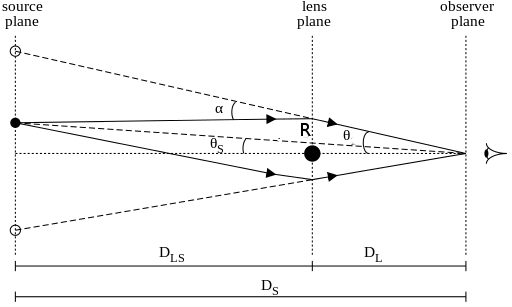
\includegraphics[width=14cm]{1_Introduccion/Gravitational_lens_geometry.png}
    \end{center}
    \caption{\small {Distribución geométrica de los elementos que conforman una lente gravitatoria.} (Fuente: \url{https://en.wikipedia.org/wiki/Einstein_radius\#/media/File:Gravitational_lens_geometry.svg})}
    \label{fig:lente}
\end{figure}

\newpage

Para realizar el estudio utilizaremos la expresión \ref{eq:bending_angle} junto con argumentos geométricos basados en la Figura \ref{fig:lente}. A partir del dibujo

\begin{equation*}
    D_S\; \theta= D_S\;{\theta}_{S} + {D}_{LS}\;\alpha,
\end{equation*}

que podemos reescribir despejando $\alpha$: 

\begin{equation}\label{eq:alpha_geometrica}
    \alpha =(\theta -{\theta}_{S})\frac{{D}_{S}}{{D}_{LS}}.
\end{equation}

La distancia entre el haz luminoso y la fuente puntual es \maths{R}. Si \maths{R} es suficientemente pequeño en comparación con \maths{D_L}, se puede realizar la aproximación

\begin{equation*}
    \frac{R}{{D}_{L}} = \sin{\theta} \approx \theta \implies R \approx \theta D_L
\end{equation*}

y el ángulo de desviación de los fotones debido a la masa gravitatoria será:

\begin{equation}\label{eq:alpha_gravitatoria}
    \alpha =\frac{4 GM}{{c}^{2}\theta {D}_{L}}.
\end{equation}

El último paso consiste en igualar la Ecuación \ref{eq:alpha_geometrica} y la Ecuación \ref{eq:alpha_gravitatoria}:

\begin{equation*}
     \frac{4 GM}{{c}^{2}\theta {D}_{L}}=(\theta -{\theta}_{S})\frac{{D}_{S}}{{D}_{LS}}
\end{equation*}

y notar que para el caso en que la masa se encuentra justo detrás de la lente, \maths{{\theta}_{S}=0}; el ángulo \maths{\theta} recibe entonces el nombre de radio de Einstein, que se denota mediante \maths{{\theta}_{E}},

\begin{equation}\label{eq:radio_einstein}
    {{\theta}_{E}}^{2}=\frac{4 GM}{{c}^{2} }\frac{D_{LS}}{D_{L} D_{S}}.
\end{equation}

Este caso particular de lente gravitatoria da lugar al fenómeno conocido como anillos de Einstein, en la que la imagen de la fuente forma un circulo centrado en el objeto lente. Los anillos de Einstein han sido detectados en varias ocasiones, pero son un fenómeno muy difícil de observar ya que los requisitos necesarios para que tengan lugar son muy improbables. Sin embargo, el concepto es importante, porque los fenómenos asociados a lentes gravitatorias fuertes se producen a escalas de \maths{{\theta}_{E}}.
Cuando \maths{D_S\gg D_L} entonces se cumple también \maths{D_S\simeq D_{LS}} y la Ecuación \ref{eq:radio_einstein} se suele aproximar como

\begin{equation}\label{eq:radio_einstein_magnitud}
    {\theta}_{E} \simeq 0.1 \times { {\left( \frac{M\;\mathrm{en}\;M_{\odot}}{D_L \;\mathrm{en\;pc}}\right)} }^{1/2}\;\mathrm{en\;arcsec},
\end{equation}

que es más adecuada para hacer cálculos teniendo en cuenta las unidades más utilizadas en astrofísica \citep{book:encyclopedia}.

\newpage

\subsection{Inferencia bayesiana.}

La inferencia bayesiana es un método racional para la actualización de creencias. Se trata de un método de razonamiento aproximado, es decir, no se considera que una determinada información sea cierta o falsa con carácter absoluto; en su lugar, se parte de una hipótesis inicial a la que se le asigna un número como medida de la credibilidad que se tiene sobre la misma y con cada nueva observación se calcula de nuevo el factor numérico con el que se cuantifica el credibilidad de la hipótesis. La herramienta matemática que se utiliza para la actualización de creencias es el Teorema de Bayes.

\subsubsection{Teorema de Bayes y teorema de las probabilidades totales.}

Uno de los conceptos fundamentales en inferencia bayesiana es el concepto de probabilidad condicional. La probabilidad condicional, es la probabilidad de que ocurra un suceso \maths{A}, dado que también tiene lugar otro suceso \maths{B}. La probabilidad condicional se escribe \maths{P(A|B)} y se lee «\resalta{probabilidad de \maths{A} dado \maths{B}}».

\begin{definition}[Probabilidad condicional]
Sean dos sucesos A y B tales que la la probabilidad de que ocurra B no sea nula, P(B)>0, se define la probabilidad de A dado B como

\begin{equation}\label{eq:prob_condicional}
    P(A|B)=\frac{P(A \cap B)}{P(B)},
\end{equation}

siendo \maths{P(A \cap B)} la probabilidad conjunta de los dos sucesos, o dicho de otra forma, la probabilidad de que se den los dos sucesos simultáneamente.

\end{definition}

A partir de la definición de probabilidad condicional podemos escribir que

\begin{equation*}
    P(A \cap B)=P(A|B)P(B)=P(B|A)P(A).
\end{equation*}

Si los sucesos son independientes entre si, \maths{P(A|B) \equiv P(A)} y \maths{P(B|A) \equiv P(B)},
y por tanto la probabilidad de ocurrencia de ambos sucesos de forma simultanea es igual al producto de la probabilidad de ocurrencia de los sucesos de forma independiente, esto es,

\begin{equation*}
    P(A \cap B)=P(A)P(B).
\end{equation*}

En el caso de que los sucesos no sean independientes, la probabilidad de que tenga lugar \maths{A} dado \maths{B} será:

\begin{equation*}
    P(A|B)=\frac{P(B|A) P(A)}{P(B)},
\end{equation*}

que es lo que se llama \textit{Teorema de Bayes\footnote{El teorema de Bayes es un resultado incontrovertible partiendo de la definición de probabilidad condicional y los axiomas de Kolmogórov.} para los sucesos A y B}.

\begin{theorem}[Teorema de Bayes]
Sea \maths{\Omega} un conjunto de sucesos %espacio muestral
compuesto por un conjunto \maths{n} de particiones mutuamente excluyentes\footnote{Tanto el Teorema de Bayes como el Teorema de la probabilidad total, son también válidos cuando existe un conjunto infinito numerable de causas disjuntas dos a dos.} ( \maths{\Omega=\{H_1,H_2,H_3...H_n\}},  \maths{H_i \cap H_j=\emptyset} siendo \maths{i\neq j}) y sea B un suceso tal que \maths{B\subset \Omega}, la probabilidad de que el suceso \maths{B} sea consecuencia de \maths{H_{i}} viene dada por

\begin{equation}\label{eq:teorema_bayes}
    P(H_i|B)=\frac{P(B|H_i)\;P(H_i)}{P(B)},
\end{equation}

donde el divisor \maths{P(B)} representa la probabilidad de que tenga lugar el suceso \maths{B}.
\end{theorem}

\begin{theorem}[Teorema de la Probabilidad Total]

Sea \maths{\Omega} un conjunto de sucesos compuesto por un conjunto \maths{n} de particiones mutuamente excluyentes  ( \maths{\Omega=\{H_1,H_2,H_3...H_n\}},  \maths{H_i \cap H_j=\emptyset} siendo \maths{i\neq j}) y sea \maths{B\subset \Omega} un suceso cualquiera del que se conocen las probabilidades condicionales \maths{P(B|H_{i})},  entonces la probabilidad del suceso \maths{B} viene dada por

\begin{equation}
    P(B)=\sum_{i=1}^{n}{P(B|H_i)P(H_i)}.
\end{equation}

\end{theorem}

\begin{figure}[htb]
    \begin{center}
         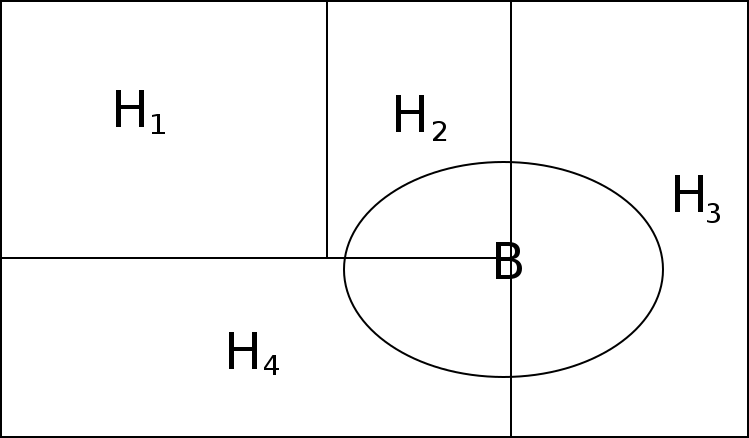
\includegraphics[width=14cm]{1_Introduccion/conjuntos.png}
    \end{center}
    \caption{\small Representación de un espacio muestral \maths{\Omega} de área unidad, constituido por cuatro particiones mutuamente excluyentes, ( \maths{\Omega=\{H_1,H_2,H_3,H_4\}},  \maths{H_i \cap H_j=\emptyset} siendo \maths{i\neq j}). En esta representación un conjunto de suceso \maths{B} equivale a una región del espacio muestral con una forma y una superficie características.} 
    
    \label{fig:conjuntos}
\end{figure}

Tanto el Teorema de Bayes como el Teorema de la Probabilidad Total admiten una interpretación gráfica. El espacio muestral \maths{\Omega} puede representarse por una superficie de área unidad, donde cada subconjunto \maths{X} tiene una probabilidad de ocurrir igual al área que ocupa  \maths{P(X)}, (Figura \ref{fig:conjuntos}). Las probabilidades condicionales se representan por las regiones que forman parte simultáneamente de dos subconjuntos del espacio muestral. En la Figura~\ref{fig:conjuntos}, el subconjunto \maths{B} es el único que solapa con otros subconjuntos. Las áreas de las regiones de \maths{B} que forman parte de uno de los subconjuntos \maths{H_i} vienen representadas por \maths{P(B|H_i)P(H_i)}, que es equivalente al área del subconjunto \maths{H_i} que forma parte de \maths{B} y que viene representado por \maths{P(H_i|B)P(B)}.

\newpage

\subsubsection{El factor de Bayes}

Supongamos que disponemos de un conjunto de datos \maths{D=\{x_1,x_2 \dots x_n\}} y dos hipótesis alterativas \maths{H_1} y \maths{H_2} para las que suponemos la función verosimilitud \maths{p(D|H_1)} y \maths{p(D|H_2)} y una \resalta{probabilidad a priori} \maths{p(H_1)} y \maths{p(H_2)}. Debido a la evidencia de los datos, se produce una trasformación de la \resalta{probabilidad a priori} en \resalta{probabilidad a posteriori} \maths{p(H_{k}|D)} a través del teorema de Bayes,

\begin{equation*}
    p(H_{k}|D)=\frac{p(D|H_{k})p(H_{k})}{p(D)}=\frac{p(D|H_{k})p(H_{k})}{p(D|H_{1})p(H_1)+p(D|H_2)p(H_2)}\qquad \qquad \qquad (k=1,2)
\end{equation*}

donde el subíndice \maths{k} indica de qué hipótesis se trata. Para elegir cuál de las dos es la hipótesis es más verosímil, se realiza el cociente de la \resalta{probabilidad a posteriori} de cada hipótesis,

\begin{equation*}
   \frac{p(H_{1}|D)}{p(H_2|D)}=\frac{p(D|H_{1})}{p(D|H_2)}\frac{p(H_{1})}{p(H_2)}.
\end{equation*}

Al cociente

\begin{equation*}
    B_{12}=\frac{p(D|H_1)}{p(D|H_2)}
\end{equation*}

se le denomina factor de Bayes.

\begin{definition}[Factor de Bayes]\label{def:factor_bayes}
El factor de Bayes se define como el cociente de la función verosimilitud de dos hipótesis alternativas

\begin{equation}\label{eq:factor_bayes}
    B_{12}=\frac{p(D|H_1)}{p(D|H_2)},
\end{equation}

donde los subíndices hacen referencia a la hipótesis 1 y 2 respectivamente.
\end{definition}


Si el valor de \maths{B_{12}} es superior a la unidad, el valor de \maths{p(D|H_1)} es superior al de \maths{p(D|H_2)} y la confianza sobre \maths{H_1} es mayor que sobre \maths{H_2}. En caso de ser inferior a la unidad, los datos refuerzan la confianza de \maths{H_2} sobre \maths{H_1}. En adelante, tomaremos los valores de la Tabla \ref{tab:bayes_interpretacion} como escala referencia.


\begin{table}[h]
\renewcommand\tablename{Tabla}
\renewcommand{\arraystretch}{1.5}
\centering
    
    \setlength{\extrarowheight}{-2pt}
    \begin{tabular}{ C{4cm} C{4cm} C{5cm} }
        \hline
        ${B}_{12}$	& $\log_{10}{(B_{12})}$	& Confianza sobre $H_1$ \\
        %\cline{1-3}
        \hline
        \hline
    \end{tabular}

    \setlength{\extrarowheight}{-1mm}
    \begin{tabular}{ C{4cm} C{4cm} C{5cm} }
        <1 &  <0 &  $H_1$ es refutada \\
        1 --- 3.2 &  0 --- $\frac{1}{2}$ &   Débil  \\
        3.2 --- 10 &  $\frac{1}{2}$ --- 1 &   Sustancial  \\
        10 --- 31.6 &  1 --- $\frac{3}{2}$ &   Fuerte  \\
        31.6 --- 100 &  $\frac{3}{2}$ --- 2 & Muy fuerte  \\
        >100 &  >2 &   Absoluta  \\


        \hline
    \end{tabular}

    \caption{\small Escala de referencia que nos relaciona el valor del factor de Bayes con la confianza que tenemos sobre la hipótesis \maths{H_1}. Se trata de la tabla de referencia utilizada por Harold Jeffreys en 1961 (consultar~\citealt{article:Robert_E_Kass_1995}).}

    \label{tab:bayes_interpretacion}
\end{table}

\newpage

En el caso particular del método de \cross\ que se va a utilizar en este trabajo, lo que pretendemos es contrastar la hipótesis \maths{H_1} de que los emparejados considerados están formados por observaciones de un mismo objeto astronómico frente a la hipótesis \maths{H_2} de que se trata de observaciones pertenecientes a dos objetos diferentes.

Si las medidas de un parámetro pertenecen a un único objeto astronómico la función densidad de probabilidad conjunta \maths{p(D|\theta,H_k)} se obtiene mediante el producto de las funciones densidad de probabilidad asociadas para cada medida \maths{p_i(x_i|\theta,H_k)} que representan la probabilidad de que una medida \maths{x_i} se corresponda exactamente con su verdadero valor \maths{\theta} y la función verosimilitud para \maths{H_1} resulta ser

\begin{equation}
    p(D|H_1)=\int p(\theta|H_1)p(D|\theta,H_1)\,d\theta=\int p(\theta|H_1)\prod_{i=1}^{n}p_i(x_i|\theta,H_1)\,d\theta,
\end{equation}

siendo \maths{p(\theta|H_1)} la densidad de \resalta{probabilidad a priori} de la hipótesis \maths{H_1}. Para el caso de la hipótesis \maths{H_2} las medidas \maths{x_i} pertenecen a distintos valores verdaderos \maths{\theta_i} por lo que la función verosimilitud de \maths{H_2} se calcula como

\begin{equation}
    p(D|H_2)=\prod_{i=1}^{n}\left[\int p({\theta}_i|H_2)p_i(x_i|{\theta}_i,H_2)\,d\theta_i \right].
\end{equation}

En los casos en que disponemos de \maths{q} conjuntos de medidas \maths{D_s} diferentes, asociados a lo distintos parámetros, dispondremos de \maths{q} factores de Bayes. Suponiendo cada uno de los parámetros que hemos elegido son igualmente válidos para determinar la verosimilitud de nuestras hipótesis, el factor de Bayes conjunto se obtiene como el producto de los factores de Bayes asociados a cada parámetro,

\begin{equation}\label{eq:bayes_multiple}
    B_{12}=B^{1}_{12}\times B^{2}_{12} \dots B^{q}_{12}=\prod_{s=1}^{q}\frac{p(D_{s}|H_1)}{p(D_{s}|H_2)}.
\end{equation}

De esta manera, cada nueva observación cambia el conjunto de valores \maths{D_s} lo que cambia la verosimilitud de cada hipótesis y en consecuencia el factor de Bayes. En esto consiste la actualización de creencias basada en el razonamiento bayesiano.

\section{Selección de las muestras}\label{sec:2_muestras}

En esta sección se explica qué es el proyecto \hatlas\ y qué es el proyecto \gama, de qué instrumentos se sirven estos proyectos para realizar las medidas y que datos nos proporcionan. Por último, se mostrará la zona en la que se produce un solapamiento de ambos cartografiados que es la zona en la podemos aplicar nuestra propuesta para la identificación del SLGs.

\subsection{Proyecto \hatlas}

\hatlas\ (\anglicismo{Herschel} Astrophysical Terahertz Large Area Survey) es el nombre de uno de los proyectos astronómicos que se fundamenta en las medidas del telescopio espacial \h. Este proyecto cubre un área total de \maths{550\;\mathrm{deg}^{2}} (la octogésima parte del cielo) requiriendo unas 600 horas de observación, lo que implica un tiempo cuatro veces mayor que todas las demás prospecciones extragalácticas de \h\ combinadas. 
Con ello se espera detectar unas \maths{2,5\times10^{5}} galaxias con desplazamientos al rojo de hasta \maths{z\sim4}, cuando el Universo tenía apenas unos pocos miles de millones de años \citep{website:hatlas}.

\subsubsection{Observatorio espacial \h.}

El observatorio espacial \h\footnote{El satélite fue nombrado en honor al astrónomo británico William Herchel conocido entre otras cosas, por el descubrimiento del planeta Urano y del espectro infrarrojo. No confundir con el telescopio óptico e IR-cercano llamado William Herschel Telescope (W\textit{H}T) que se encuentra en el Observatorio del Roque de los Muchachos en la isla de La Palma.} es un proyecto de la ESA (European Space Agency), lanzado el día 14 de mayo de 2009 junto con el satélite espacial Planck. El periodo de vida útil terminó el día 29 de Abril de 2013 cuando agotaron los 2200 litros de helio superfluido que utilizaba como refrigerante. Se encontraba situado en el punto \maths{{L}_{2}} de Lagrange, a unos \maths{1.5 \times {10}^{6}\;\mathrm{km}} de la Tierra; este es un punto de especial interés para colocar observatorios espaciales, puesto que los cuerpos situados ahí mantienen la misma posición relativa entre el Sol y la Tierra.
Se trata del mayor telescopio infrarrojo espacial que se ha construido hasta el momento. Dispone de un único espejo de 3.5 metros de diámetro y de varios instrumentos diseñados para realizar observaciones en el rango espectral que va desde el IR lejano hasta la banda submilimétrica, \microm{55-672}. 

Los tres instrumentos del observatorio espacial son:

\vspace{-3mm}
\begin{itemize}
    
    \item \spire\ (Spectral and Photometric Imaging Receiver) \cite{website:spire_website}.
    
    Se trata de una cámara fotométrica y un espectrómetro de transformada de Fourier. Ambos instrumentos operaban refrigerados por He líquido superfluído a una temperatura de \maths{\sim~0.3\;\mathrm{K}}. \spire\ se construyó con dos objetivos, el estudio de la formación de estrellas y la formación de galaxias. En ambos casos está involucrado un proceso similar de absorción de la luz visible y UV procedente de las estrellas y posterior remisión de radiación IR por el gas y polvo interestelar, con una longitud de onda de unos \microm{100}.
    
    La cámara opera simultáneamente en tres bandas del espectro electromagnético, centradas en \microm{250}, \microm{350}, y \microm{500}, con una resolución angular de \maths{20-30\:\mathrm{arcsec}} y un campo de visión de \maths{4\times8} minutos de arco. El sensor cuenta con 270 píxeles.
    
    El espectrómetro tiene una resolución espectral de \maths{300\;\mathrm{km\;{s}^{-1}}}, cubre el rango de frecuencias entre \microm{200-670}   y su resolución angular es de \maths{20-50\:\mathrm{arcsec}}. El campo de visión es de \maths{2.6\times2.6} minutos de arco. En cuanto al detector, dispone de 56 píxeles.
     
    El instrumento ha sido construido por un consorcio internacional de 18 instituciones, de 8 países, liderado por el Dr. Matt Griffin del Cardiff Institute (AIG)\citep{website:h_instrumets}.
    
    \item \pacs\ (Photodetecting Array Camera and Spectrometer) \citep{website:pacs_website}.
    
    Al igual que \spire, \pacs\ está formado por dos instrumentos independientes; una cámara y un espectrómetro integral de campo. 
    
    La cámara toma imágenes en dos bandas de forma simultánea, a \microm{60-85} o \microm{85-130} y a \microm{130-210} mediante dos sensores bolométricos. Los sensores bolométricos están formados por un array de \maths{32\times16} y de \maths{64\times32} respectivamente. La resolución angular es de \maths{5\:\mathrm{arcsec}} y el campo de visión es de \maths{1.75\times3.5} minutos de arco. El límite de detección está en \maths{3\;m\mathrm{Jy}}\footnote{El Jansky (Jy) es una unidad de densidad de flujo espectral o irradiancia, especialmente utilizada en astronomía que no pertenece al Sistema Internacional de Unidades (SI). Es equivalente a \maths{{10}^{-26}\:\mathrm{W\:m^{-2} {Hz}^{-1}}}.}.
    
    Al espectrómetro también trabaja simultáneamente en dos frecuencias, en \microm{57-105} y \microm{105-210}. Los detectores están compuestos por un array de \maths{5\times5} y de \maths{16\times25} sensores de Ge-Ga. La resolución espectral es de \maths{150-200\;k\mathrm{m\;{s}^{-1}}}, la resolución espacial es de \maths{10\:\mathrm{arcsec}} y el campo de visión de \maths{50\times50}. Para \maths{\frac{\lambda}{\Delta \lambda}\sim1500} la sensibilidad es de \maths{5\times{10}^{-18}\mathrm{W\;{m}^{-2}}}.
    
    El instrumento ha sido construido por un consorcio internacional de 12 instituciones pertenecientes a 6 países, liderado por el investigador Dr. Albrecht Poglitsch del Max-Planck-Institute\citep{website:h_instrumets}.
    
    
    \item \hifi\ (Heterodyne Instrument for the Far Infrared) \citep{website:hifi_website}.
    
    Se trata de un espectrómetro de muy alta resolución espectral (0.02-0.7 km/s) que trabaja entre los \microm{157-625}. Tiene una resolución espacial de \maths{13-40\:\mathrm{arcsec}}. La temperatura de trabajo se encuentra entre los \kelvin{2-10}.
    
    Al igual que los instrumentos anteriores, este ha sido construido por un consorcio internacional de 26 instituciones pertenecientes a 11 países diferentes. El líder principal del proyecto en este caso es Thijs de Graauw del Stichting Ruimte Onderzoek Nederland (SRON)\citep{website:h_instrumets}.


\end{itemize}

\subsubsection{Catálogo \hatlas\ DR1.}\label{subsec:catalogo_hatlas}

El lanzamiento de datos \hatlas\ DR1 (Data Release 1) fue publicado el 28 de junio de 2016. Los detalles sobre su contenido se encuentran en las publicaciones \cite{article:valiente_2016} y
\cite{article:bourne_2016}. Este lanzamiento de datos incluye varios mapas y archivos adicionales; en este trabajo se utilizará únicamente el fichero {\small HATLAS\_DR1\_CATALOGUE\_V1.2.FITS}\footnote{Dirección de descarga: \url{http://www.h-atlas.org/public_data/DR1/HATLAS_DR1_CATALOGUE_V1.2.FITS}}.
Se compone de tres campos centrados en ascensión recta 09h, 12h y 14.5h sobre el ecuador celeste (denominadas por el proyecto Bloques, Figura~\ref{fig:TOPCAT_HATLAS}) que cubren cubren un área de total de  \maths{161\;\mathrm{{deg}^{2}}} con 120230 fuentes identificadas en 3 bandas fotométricas.

\begin{figure}[htb]
    \begin{center}
         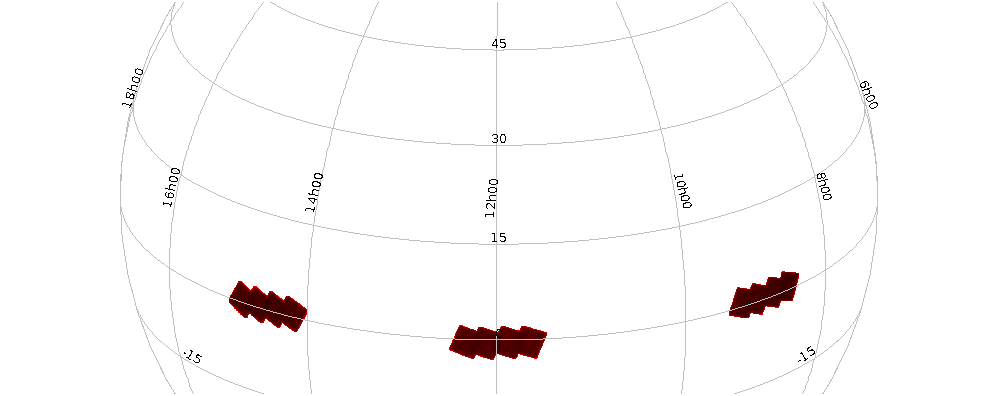
\includegraphics[width=14cm]{2_Muestras/atlas.png}
    \end{center}
    
    \caption{\small Representación de los objetos publicados en el catálogo \hatlas\ Data Release 1 (DR1) en coordenadas ecuatoriales utilizando el programa TOPCAT\footnotemark (Tool for OPerations on Catalogues And Tables). De derecha a izquierda, cada una de las tres regiones recibe el nombre de Bloque 2, Bloque 3 y Bloque 4. (ver: \href{website:hatlas_fields}{http://www.h-atlas.org/survey/fields})}.
    \label{fig:TOPCAT_HATLAS}
\end{figure}
\footnotetext{Página web del proyecto que desarrolla TOPCAT: \url{http://www.star.bris.ac.uk/\%7Embt/topcat/}}

A continuación se muestra una breve descripción de las columnas del catálogo\footnote{Para una descripción completa de cada una de las columnas del fichero consultar la dirección:

\url{http://www.h-atlas.org/public_data/DR1/HATLAS_DR1_CATALOGUE.COLUMNS}} que son relevantes en este trabajo:

\vspace{-3mm}
\begin{itemize}
    \setlength\itemsep{-1mm}
    \item HATLAS\_IAU\_ID: Contiene el identificador de la fuente astronómica del catálogo \hatlas\ asignado por la IAU (International Astronomy Union).
    \item RA: Ascensión recta, en grados, de la fuente astronómica obtenida a partir de los datos de la banda de \microm{250}.
    \item DEC: Declinación, en grados, de la fuente astronómica obtenida a partir de los datos de la banda de \microm{250}. 
    
    \item F250: Flujo de la fuente, en Jy, de la banda de \microm{250}.  El límite de detección \maths{5\sigma}\footnote{Una desviación estándar de \maths{1\sigma} significa que si asumimos una distribución normal de los valores posibles que puede tomar una medida respecto a su valor verdadero \maths{x}, hay un probabilidad de en torno al \maths{68\%} de que esta se encuentre en el intervalo \maths{x\pm\sigma}. El límite de detección \maths{5\sigma} es un criterio para determinar cuándo se ha detectado una fuente sobre la señal de ruido de fondo.} de esta banda se encuentra en \maths{33.5\;\mathrm{mJy}} \citep{article:Nuevo_2012}
    
    \item F350: Flujo, en Jy, de la banda de \microm{350}. El límite de detección \maths{5\sigma}, \maths{37.7\;\mathrm{mJy}}.
    
    \item F500: Flujo, en Jy, de la banda de \microm{500}. El límite de detección \maths{5\sigma}, \maths{44.0\;\mathrm{mJy}}.
    
    \item E250: Desviación estándar (\maths{1\sigma}) del flujo para la observación de un objeto en la banda \microm{250}. 
    \item E350: Desviación estándar del flujo en la banda \microm{350}.
    \item E500: Desviación estándar del flujo en la banda \microm{500}.
    \item \maths{\mathrm{GSQ\_FLAG}}: Se hace una clasificación del tipo de objeto basada diagramas de color g-i~/~J-K además de los criterios de PSF~/~magnitud de modelo de banda r \citep{article:bourne_2016}. La columna contiene un entero con tres posibles valores, cuyo significado es el  siguiente: 0=galaxia, 1=estrella, 2 y 3=cuásar.
    
    \item \maths{\mathrm{Z\_SPEC}}: Contiene los valores del \rt\ de algunos de los objetos del catálogo \hatlas. Aquellos cuyo valor es desconocido y no ha podido calcularse fotométricamente aparecen con valor -99.		
    \item \maths{\mathrm{Z\_QUAL}}: Etiqueta que indica el nivel de confianza \maths{Q_h} que se tiene sobre el valor del \rt\ que aparece en la columna \maths{\mathrm{Z\_SPEC}}. Los objetos cuya etiqueta tiene un valor \maths{\geq3}, tienen \anglicismo{redshifts} espectroscópicos considerados de confianza. El proyecto indica que los \anglicismo{redshifts} fotométricos han sido calculados mediante ANNz; por ese motivo hemos tratado a aquellas medidas con un factor de calidad 1 o 2 como si hubieran sido obtenidos mediante ANNz. 
    \item \maths{\mathrm{Z\_SOURCE}}: Indica la fuente de procedencia de los valores del \rt\ del catálogo. El código es el siguiente: 1- SDSS DR7, 2- 6dFGS, 4- 2SLAQ-QSO, 8- 2SLAQ-LRG, 16- GAMA HATLAS filler targets, 32- GAMA Main Survey, 64- 2dFGRS, 128- SDSS DR10, 256- Wigglez, 512- GAMA (que no se encuentran actualmente en TilingCat de GAMA-II)
\end{itemize}

\newpage

De las 120230 fuentes del catalogo DR1 solo 28389 tienen un \rt\ con factor de calidad \maths{Q_h\geq3} y 931 factor de calidad \maths{Q_h=1\vee2} (ver fig: \ref{fig:histograma_z_hatlas}). Al resto de fuentes, cuyo \rt\ es desconocido, les aplicaremos el algoritmo descrito en la sección \ref{sec:3_redshift_hatlas}. Si estos resultan ser galaxias (según la clasificación de la columna \maths{\mathrm{GSQ\_FLAG}}) y el ajuste proporciona un valor comprendido entre \maths{1<z<3.5} aceptaremos el valor del ajuste como medida válida de \maths{z}. 

En cuanto a la desviación estándar de las medidas del \rt\ el proyecto no proporciona su valor directamente. Para conocer su valor tendríamos que conocer los detalles de cómo se ha obtenido el \rt\ dependiendo de la procedencia de las medidas, lo cual implica mucho tiempo, que no está justificado emplear en este trabajo de final de grado. Una alternativa hubiera sido buscar los objetos en otra base de datos como NED (NASA/IPAC Extragalactic Database: \url{http://ned.ipac.caltech.edu/}) o SIMBAD (Set of Identifications, Measurements, and Bibliography for Astronomical Data: \url{http://simbad.u-strasbg.fr/simbad/}) ya que existen rutinas ya implementadas en \python\ para este tipo de tareas. Sin embargo, nos podemos encontrar en la situación de que estas bases de datos tampoco dispongan de las desviaciones estándar de todos los objetos en los que estamos interesados\footnote{Se ha realizado una búsqueda individual de unos cuantos objetos del catálogo \hatlas\ (30 objetos), cuyo \rt\ tiene \maths{Q_h\geq3} a partir del identificador asignado por la IAU en la base de datos NED y se ha encontrado el valor de \maths{z} y \maths{{\sigma}^{z}} solamente para unos pocos casos (3).}. Por ese motivo, la solución que se ha adoptado en este trabajo ha sido dividir las medidas proporcionadas por \hatlas\ en dos grupos. Por una parte tenemos los objetos cuyo factor de calidad es \maths{Q_h=1\vee2}. Estos objetos suponemos que se han obtenido todos ellos mediante ANNZ, por lo que si las medidas se encuentran en el rango \maths{0<z<0.7}, es razonable suponer para todas ellas  \maths{{\sigma}^{z}=0.023} a partir del estudio realizado por \cite{article:annz}. En el caso de que el factor de calidad sea \maths{Q_h\geq3} la desviación estándar de las medidas se obtendrá a partir del ajuste que se muestra en la Figura~\ref{fig:ajuste_error_gama} (asignar la misma desviación estándar a los desplazamientos al rojo espectroscópicos de los proyectos \gama\ y \hatlas\ está justificado porque la procedencia de estas medidas es la misma en muchos casos). El hecho de que una medida tenga un factor de calidad más alto que otra, no quiere decir que el valor de las desviaciones estándar sea diferente. El factor de calidad indica la confianza subjetiva que tienen los autores del catálogo sobre las medidas del \rt\ \citep{article:Driver_2011}. La confianza puede ser baja por cualquier motivo.

En resumen, para asignar los errores a las medidas del \rt\ de los objetos de \hatlas\, se ha decidido lo siguiente:

\vspace{-3mm}

\begin{itemize}
    \item Si el factor de calidad de la medida del \rt\ por el proyecto \hatlas\ es \maths{\geq3}, el \rt\ es espectroscópico y la desviación estándar se obtiene a partir de la expresión \maths{{\sigma}^{z}=1.1\times{10}^{-4}\times(1+z)}.
    
    \item Si el factor de calidad \maths{Q_h=1\vee2}, se tratará a la medida como si hubiera sido obtenida mediante ANNZ. Si su valor pertenece al intervalo \maths{0<z<0.7} se le asignará una desviación estándar \maths{{\sigma}^{z}=0.023}.
    
    \item Si el \rt\ es desconocido por el proyecto \hatlas\ y el ajuste obtenido mediante el algoritmo descrito en la Sección~\ref{sec:3_redshift_hatlas} se encuentra en el intervalo \maths{1<z<3.5} consideraremos válido este valor y le asignaremos una desviación estándar  \maths{{\sigma}^{z}=0.115\times(1+z)} .
\end{itemize}

\begin{figure}[htb]
    \begin{center}
         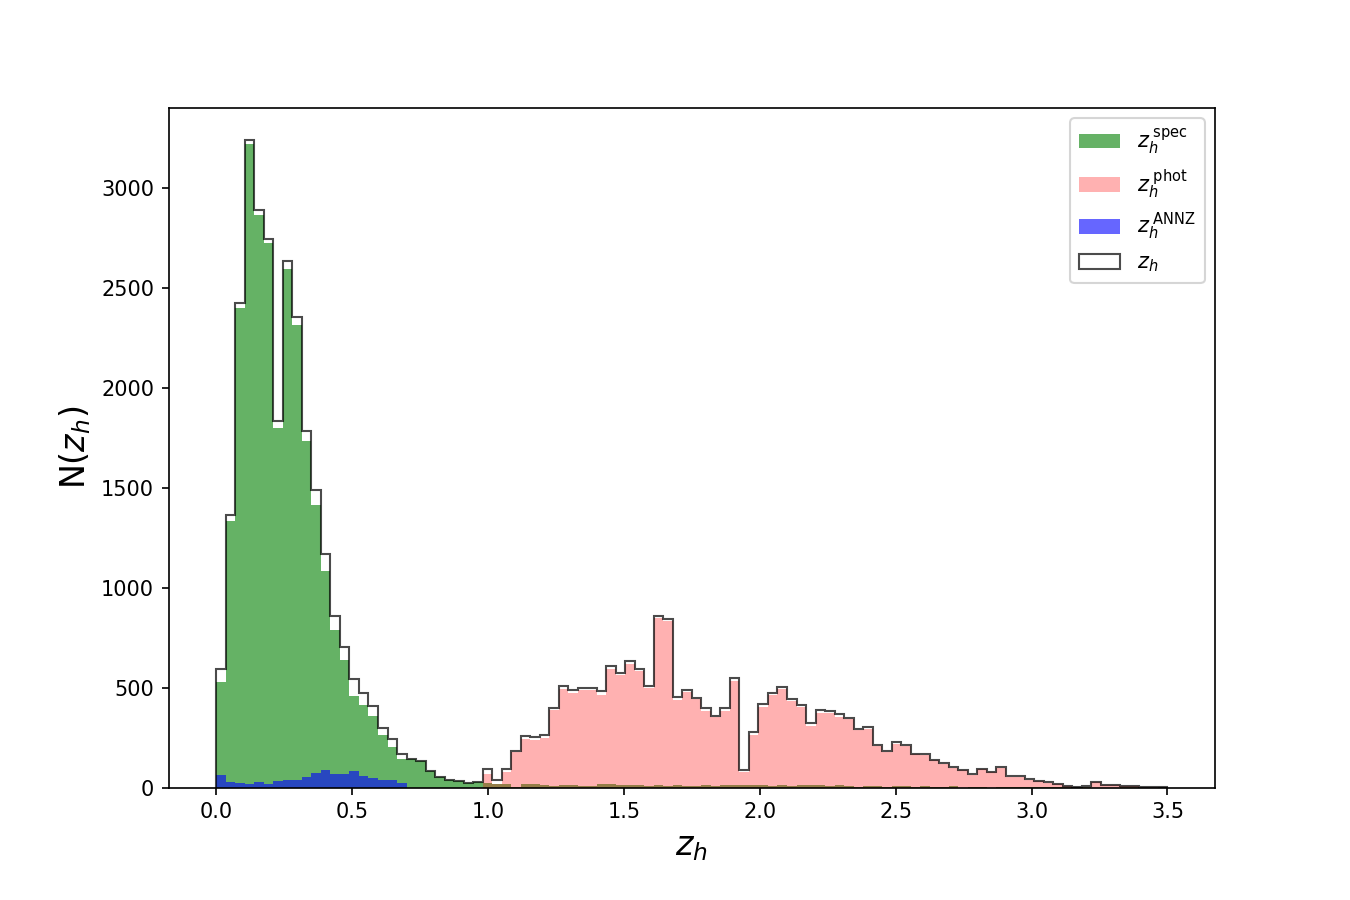
\includegraphics[width=15cm]{2_Muestras/histograma_z_hatlas_disponible.png}
    \end{center}
    \vspace*{-10mm}
    \caption{\small Histograma del \rt\ de los 47844 fuentes del proyecto \hatlas\ de los que el disponemos medidas o estimaciones  razonables del \rt\ \maths{z_{h}} de un total de 120230 para el catálogo completo. Estas fuentes se encuentran representadas en tres categorías; objetos de los que se dispone de una medida espectroscópica de confianza \maths{N({z_{h}^{\mathrm{spec}}})=28389}, objetos cuyo \rt\ tiene un nivel de confianza \maths{Q_h=1\vee2} (tratados como si hubieran sido obtenidos mediante ANNZ) \maths{N(z_{h}^{\mathrm{annz}})=931} y objetos cuyo \rt\ ha sido obtenido mediante el método descrito en la Sección~\ref{sec:3_redshift_hatlas} \maths{N(z_{h}^{\mathrm{phot}})=18524}. }
    \label{fig:histograma_z_hatlas}
\end{figure}

Por último, otro dato que es de gran importancia es el valor de la resolución angular. El valor de la FWHM\footnote{FWHM es la anchura a media altura (Full Width at Half Maximum) de la dispersión de las medidas suponiendo que se trata de una distribución normal.} para el catálogo \hatlas\ es de \maths{17.98\;\mathrm{arcsec}} en la banda de \microm{250}\footnote{El dato se encuentra en: \url{http://www.h-atlas.org/public_data/HATLAS_SDP_catalogue.README}}. Nosotros obtenemos el valor de la desviación típica como \maths{{\sigma}_{h}^{p}=\mathrm{FWHM}\times(2\sqrt{2\ln{2}})^{-1}\sim7.63\:\mathrm{arcsec}}.

\newpage

\subsection{Proyecto \gama}

\gama\ (Galaxy And Mass Assembly) es un proyecto internacional que hace uso de los más modernos observatorios espaciales y terrestres con el objetivo principal de estudiar estructuras de entre 1 kpc a 1 Mpc, lo cual incluye escalas que abarcan desde la estructura interna de las galaxias hasta cúmulos de galaxias \citep{website:Gama}. Concretamente se pretende mejorar en tres asuntos clave respecto a otros estudios:

\vspace{-3mm}

\begin{itemize}
    \setlength\itemsep{-1mm}
    
    \item Mejora de la la eficiencia espectroscópica, permitiendo el muestreo integral desde galaxias para \rt\ intermedios y mostrar esa información en un mismo estudio.
 
    \item Mejorar la resolución espacial para estudiar la estructura de las galaxias próximas y los procesos de formación galáctica.
 
    \item Mejorar el rango de la cobertura espectral.
 
\end{itemize}

Es destacable el amplio rango espectral que cubre el proyecto que abarca desde la región de Rayos X, hasta la región de radio de alta frecuencia (90 cm).  GAMA, hace uso de una amplia variedad de medidas procedentes de otros proyectos, entre los cuáles destacan:

\vspace{-3mm}

\begin{itemize}
    \setlength\itemsep{-1mm}
    
    \item Cartografiados públicos: Sloan Foundation 2.5m SDSS
    
    \item United Kingdom Infrared Telescope (UKIRT) UKIDSS-LAS
    
    \item Campañas GAMA: Galaxy Evolution Explorer (GALEX) GALEX-GAMA
    
    \item Giant Metrewave Radio Telescope (GMRT) GMRT-GAMA
    
    \item Cartografiados relacionadas con GAMA:  VLT Survey Telescope (VST) KiDS
    
    \item Visible and Infrared Survey Telescope for Astronomy (VISTA) VIKING
    
    \item The Canada France Hawaii Lensing Survey  (CFHTLenS)
    
    \item Observatorio Espacial Herschel H-ATLAS
    
    \item Australian Square Kilometre Array Pathfinder (ASKAP) DINGO
    
    \item X-ray Spectroscopy Mission and the X-ray Multi-Mirror Mission (XMM-Newton) XMM-XXL
    
    \item Wide-Field Infrared Survey Explorer (WISE)
    
\end{itemize}

El estudio espectroscópico de \gama\ cubre aproximadamente  \maths{3\times{10}^{5}} galaxias de hasta magnitud 19.8, repartidas en un área de \maths{286\;\mathrm{{deg}^{2}}}. Estas medidas son fruto de 210 noches de observación en un periodo de 7 años, desde 2008 hasta 2014, realizadas con el espectrógrafo AAOmega en el telescopio Anglo-Australiano (AAT) por miembros del equipo de GAMA. Estos datos han sido completados por datos procedentes de estudios previos como el Sloan Digital Sky Survey (SDSS), el 2dF Galaxy Redshift Survey (2dFGRS) y el Millennium Galaxy Catalogue (MGC). 

\subsubsection{Catálogo \gama\ I}

El proyecto \gama\ ha publicado dos bases de datos denominadas GAMA DR1 y GAMA DR2. La primera, fue publicada el 25 de junio de 2010 y contiene el \rt\ y otra información adicional de 114441 objetos repartidos por tres regiones, denominadas G09, G12 y G15 (Estas solapan parcialmente con las regiones que cubre el proyecto \hatlas). Estas regiones tienen una forma aproximadamente rectangular de \maths{12\times4\;\mathrm{deg}} y están situadas sobre el ecuador celeste, sumando un total de \maths{\sim144\;\mathrm{{deg}^{2}}}. El límite de magnitud para estas fuentes es de 19.4 en las regiones G09 y G15 y 19.8 en la región G12.

La segunda publicación cubre el mismo área del cielo, pero representa un conjunto de objetos más reducido de que la primera, con más información adicional. 
El límite de magnitud de los objetos pertenecientes a esta publicación es de 19.0 en la región G09 y G12 y de 19.4 para la región G15. Los datos de la región G15 son prácticamente los mismos en ambas publicaciones. 

\vspace{3mm}

\begin{figure}[htb]
    \begin{center}
         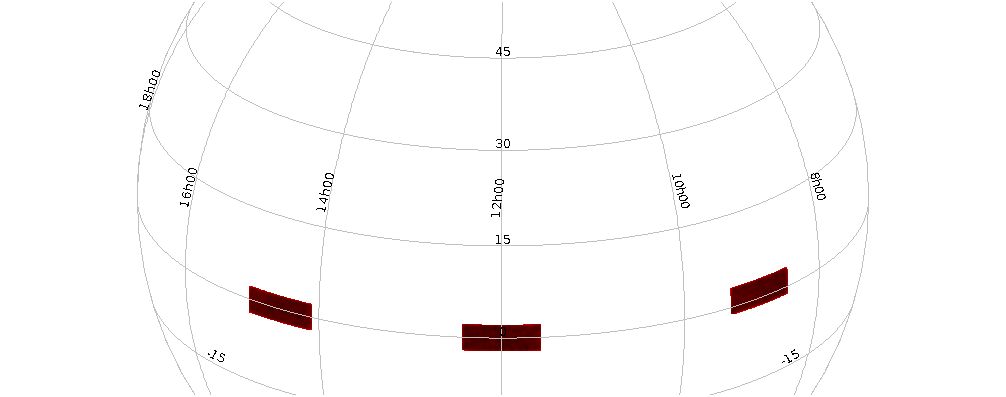
\includegraphics[width=14cm]{2_Muestras/gama.png}
    \end{center}
    
    \caption{\small Representación de los objetos publicados en el catálogo GAMA DR1 en coordenadas ecuatoriales utilizando el programa TOPCAT. De derecha a izquierda, las regiones reciben los nombres G09, G12, G15.} 
    \label{fig:TOPCAT_GAMA}
\end{figure}

En este trabajo usaremos los datos de la publicación \gama\ DR1\footnote{El fichero con los datos de esta publicación se encuentra alojado en la dirección: \url{http://www.gama-survey.org/dr1/data/GamaCoreDR1_v1.fits}}. La descripción completa de las columnas del catálogo se encuentra en el artículo \cite{article:Driver_2011}; nosotros mostramos aquí una descripción solo de las columnas que vamos a utilizar:

\begin{itemize}
    \setlength\itemsep{-1mm}
    \item GAMA\_IAU\_ID: Identificador de la fuente astronómica del catalogo GAMA asignado por la IAU.
    \item RA: Ascensión recta, en grados, de la fuente astronómica obtenida del proyecto SDSS DR6.
    \item DEC: Declinación, en grados, de la fuente astronómica obtenida del proyecto SDSS DR6.
    \item Z\_HELIO: Valores del \rt\ heliocéntrico proporcionados por el proyecto \gama. Aquellas medidas que no se encuentran disponibles se indican con un -2 o 9999.
    \item Z\_QUALITY: Etiqueta que indica la confianza que se tiene sobre los valores presentes en la columna Z\_HELIO. Nos referiremos a esta etiqueta como \maths{Q_g}.
    \item Z\_SOURCE: Etiqueta que indica la  procedencia de la medida del \rt. El criterio es el siguiente: 1 = SDSS DR6, 2 = 2dFGRS, 3 = MGC, 4 = 2SLAQ-LRG, 5 = GAMA, 6 = 6dFGS, 7 = UZC, 8 = 2QZ, 9 = 2SLAQ-QSO, 10 = NED.
    
    
\end{itemize}

El proyecto \gama\ solo proporciona medidas espectroscópicas del \rt. De las 114441 fuentes presentes en GAMA DR1, solo 59479 tienen \rt\ con factor de calidad \maths{Q_g\geq3} (los factores de calidad de los proyectos \gama\ y \hatlas\ son independientes). Los detalles relativos al factor de calidad asignado a las medidas espectroscópicas del proyecto \gama\ se encuentran en \cite{article:Driver_2011}. 

\vspace{-4mm}

\begin{figure}[htb]
    \begin{center}
         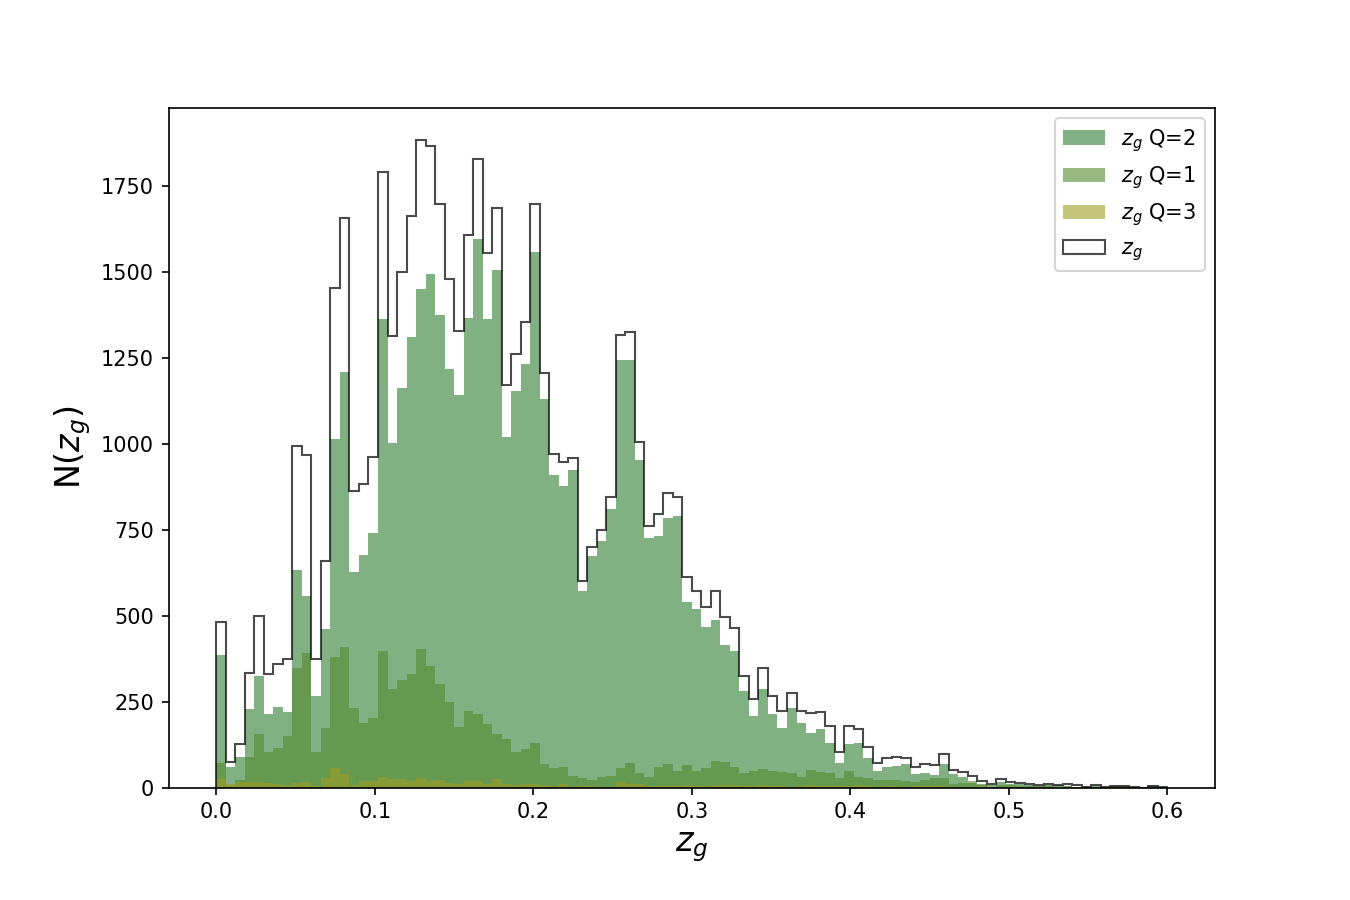
\includegraphics[width=15cm]{2_Muestras/histograma_z_gama_disponible.png}
    \end{center}
    \vspace*{-10mm}
    \caption{\small Histograma que representa el número de objetos del proyecto \gama\ de los cuales su \rt\  está disponible, \maths{N(z_{g})=59479}. Todas las medidas del \rt\ son espectroscópicas, no obstante, el proyecto les ha asignado distintos factores de calidad. Cuanto menor es el factor \maths{Q_g} mayor es la confianza que se tiene sobre esa medida. Hay 9197 con factor de calidad \maths{Q_g=1}, 49416 con \maths{Q_g=2}, y 866 con \maths{Q_g=3}. Hay objetos en ste catálogo con \maths{z_g > 0.6}, pero pero no se encuentran aquí, porque suponen una parte muy pequeña de la población representada.}
    \label{fig:histograma_z_gama}
\end{figure}

Al igual que ocurre con \hatlas, este proyecto tampoco proporciona la desviación estándar asociada a las medidas del \rt. En la Figura~\ref{fig:ajuste_error_gama} se muestra el ajuste que se ha realizado para estimar la dependencia \maths{{\sigma}^{z}} con \maths{z} a partir de una muestra de 20 objetos del catálogo \gama, con factor de calidad \maths{Q_g}=5 cuyas medidas se encuentran disponibles en NED (ver Tabla~\ref{apendice:tab:sigmas}).

\begin{figure}[htb]
    \begin{center}
         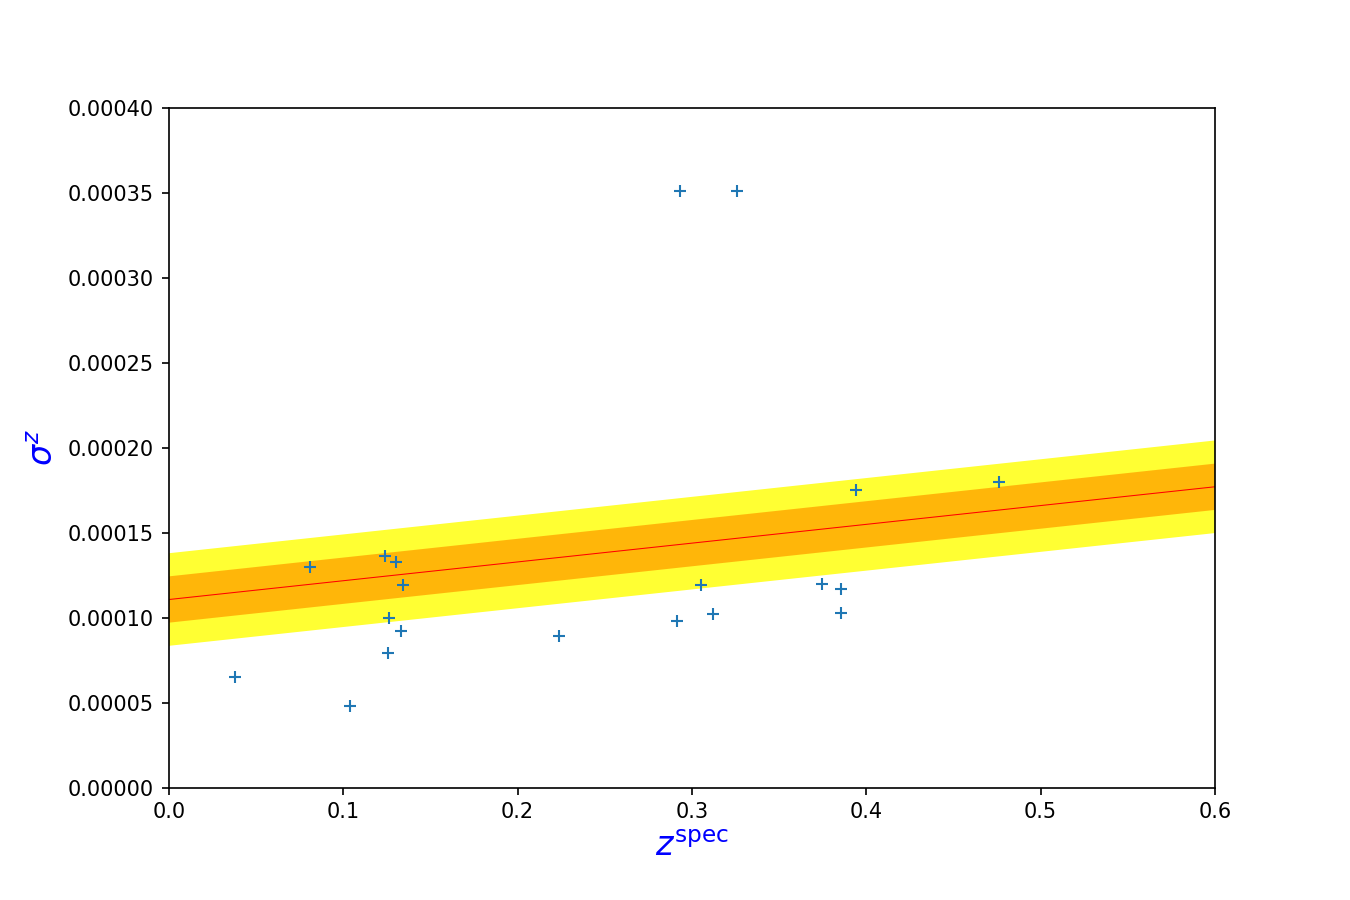
\includegraphics[width=14cm]{2_Muestras/ajuste_errores_z.png}
    \end{center}
    \vspace*{-10mm}
    \caption{\small Representación de la desviación estándar del \rt, \maths{{\sigma}^{z}} en función del \rt\ espectroscópico, \maths{{z}^{\mathrm{spec}}} de una muestra de 20 objetos del catálogo \gama\ (los 20 primeros objetos que aparecen en la Tabla~\ref{tab:ajuste_error_gama}). La recta se ha obtenido mediante un ajuste lineal de la forma \maths{{\sigma}^z= a\times(1+z)} con \maths{a} como parámetro de libre. El parámetro resultante del ajuste ha sido \maths{a=(11 \pm 1)\times{10}^{-5}}.
    \label{fig:ajuste_error_gama}}
\end{figure}

En el caso de las posiciones proporcionadas por \gama\ el valor de la \maths{\mathrm{FWHM}=0.7\;\mathrm{arcsec}}, por lo que el valor de la desviación típica en este caso es \maths{{\sigma}_{g}^{p}\sim0.30\;\mathrm{arcsec}} \citep{article:driver_2009,article:driver_2008}.

\subsection{Región de solapamiento de ambos catálogos}

Los proyectos \gama\ y \hatlas\ cubren  áreas pequeñas en comparación con la superficie total de la esfera sobre el ecuador celeste (ver Figura~\ref{fig:TOPCAT_GAMA} y Figura~\ref{fig:TOPCAT_HATLAS}). Esto permite proyectar estas regiones sobre el plano sin cambiar demasiado el valor de la superficie\footnote{La superficie de una sección esférica definida entre los paralelos 0 y
DEC y los meridianos 0 y
AR viene dada por la expresión \maths{
A_{sr}=\mathrm{AR}\times\sin{(\mathrm{DEC})}}. Si tomamos por ejemplo la región G12 que se encuentra entre los paralelos DEC=-2 y DEC=2 y meridianos RA=174 y RA=186 el área que obtenemos con la ecuación anterior es de \maths{A_{sr}\simeq0.014618666993941102\:\mathrm{sr}\simeq47.99025283641695\:\mathrm{deg^2}} mientras que al proyectar sobre una superficie plana es \maths{48\:\mathrm{deg^2}}. La diferencia entre el valor real y la aproximación es por tanto inferior a \maths{0.01\:\mathrm{deg^2}}.}.

Las áreas cubiertas por \gama\ tienen una forma que se aproxima muy bien a un rectángulo, mientras las regiones de \hatlas\ forman un polígono de 16 vértices con el que resulta más difícil trabajar. Por ese motivo, para calcular las áreas de las regiones de intersección de ambos catálogos se ha recurrido a la función \texttt{area\_region} que se encuentra definida en el Apéndice~\ref{apendice:codigo:get}. De forma resumida, lo que se hace es proyectar los puntos sobre un plano y crear una red con celdas cuadradas. Después se hace un conteo de las celdas que tienen objetos de \gama\ y de \hatlas\ a una distancia de su centro igual o inferior a la mitad de la diagonal de la celda. De esta manera se obtiene el área de las regiones de solapamiento como el producto del área de la celda por el número surgido del conteo.

Al aplicar el algoritmo para determinar el área de las regiones cubiertas por cada uno de los catálogos vemos que existen diferencias de entorno a \maths{1\:\mathrm{deg^2}} con las áreas que consideramos consideramos correctas. A partir de esta observación hemos estimado un área de intersección entre ambos catálogos de \maths{130\pm1\:\mathrm{deg^2}}.

\newpage

\begin{figure}[H]
\captionsetup[subfigure]{labelformat=empty}
%Ausencia de espacios entre los subfloat, figuras en paralelo
  \begin{center} 
  
    \subfloat[]{
     \label{subfig:region_1}
      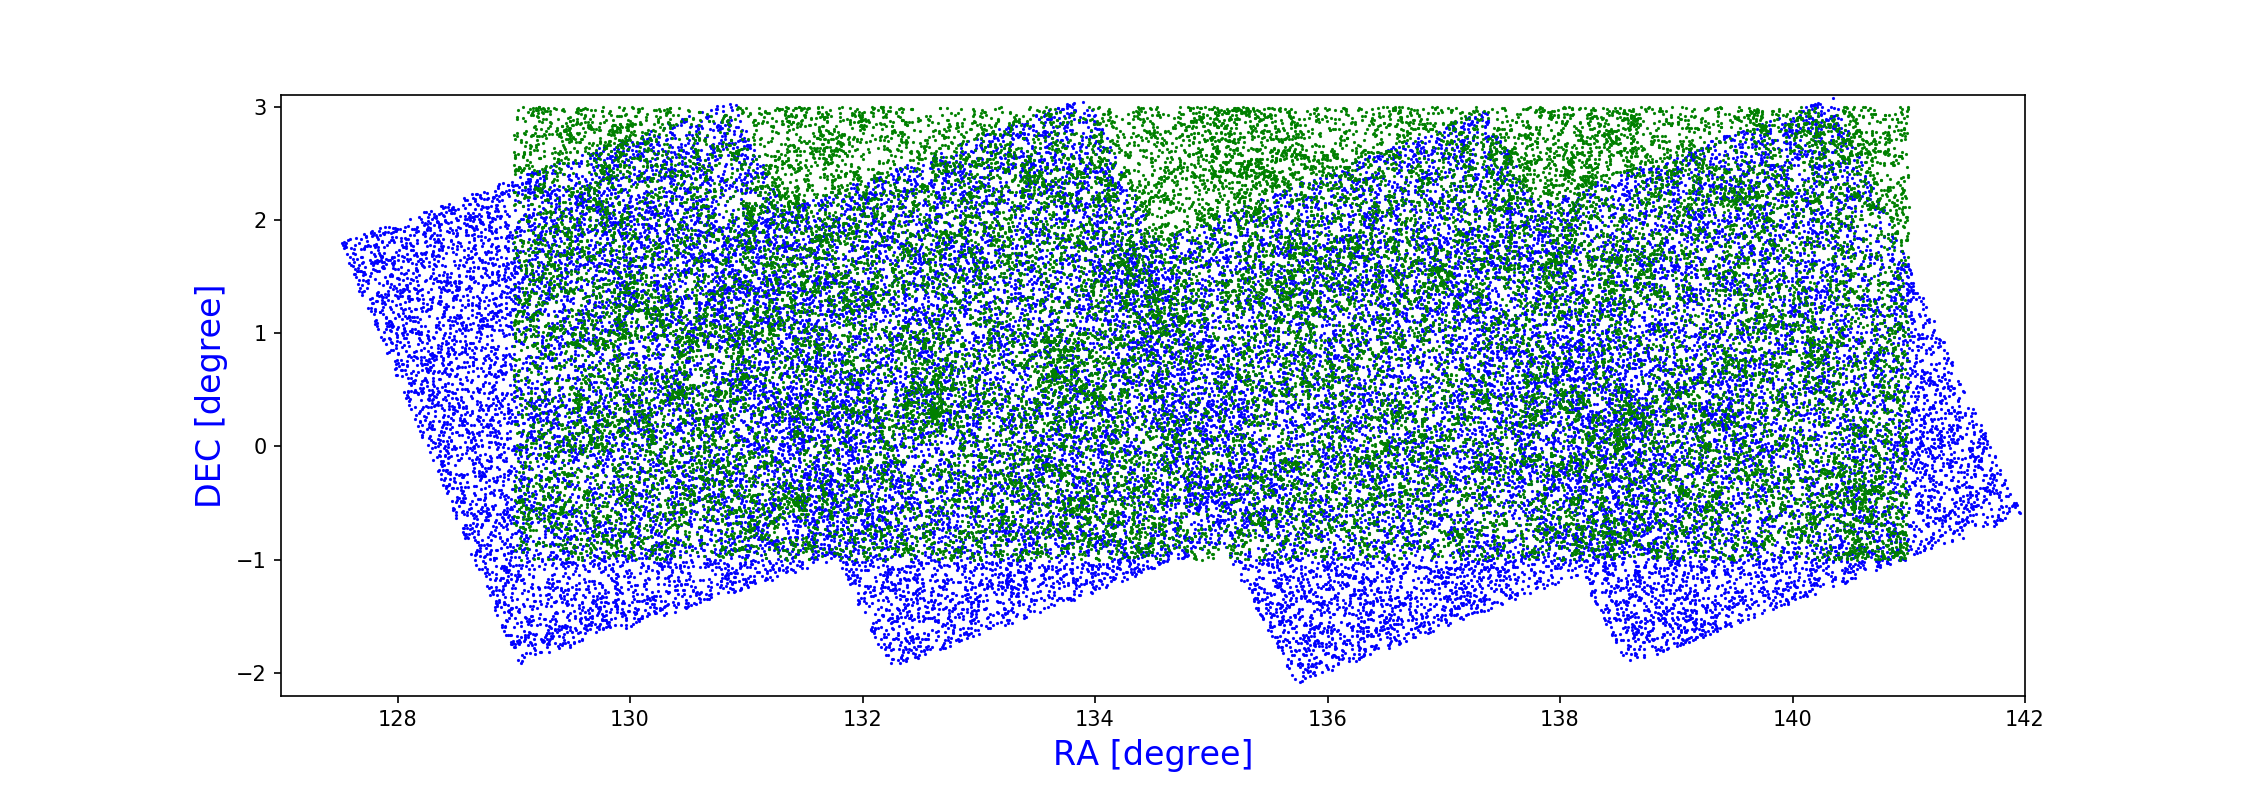
\includegraphics[width=\textwidth]{2_Muestras/region_1.png}}
      \vspace*{-10mm}
      \caption*{\small G09 (48.56 \maths{\mathrm{{deg}^{2}}}, verde) y Bloque 2 (54.15 \maths{\mathrm{{deg}^{2}}}, azul). Solapamiento: 42.96 \maths{\mathrm{{deg}^{2}}}.}
      
    \subfloat[]{
     \label{subfig:region_2}
      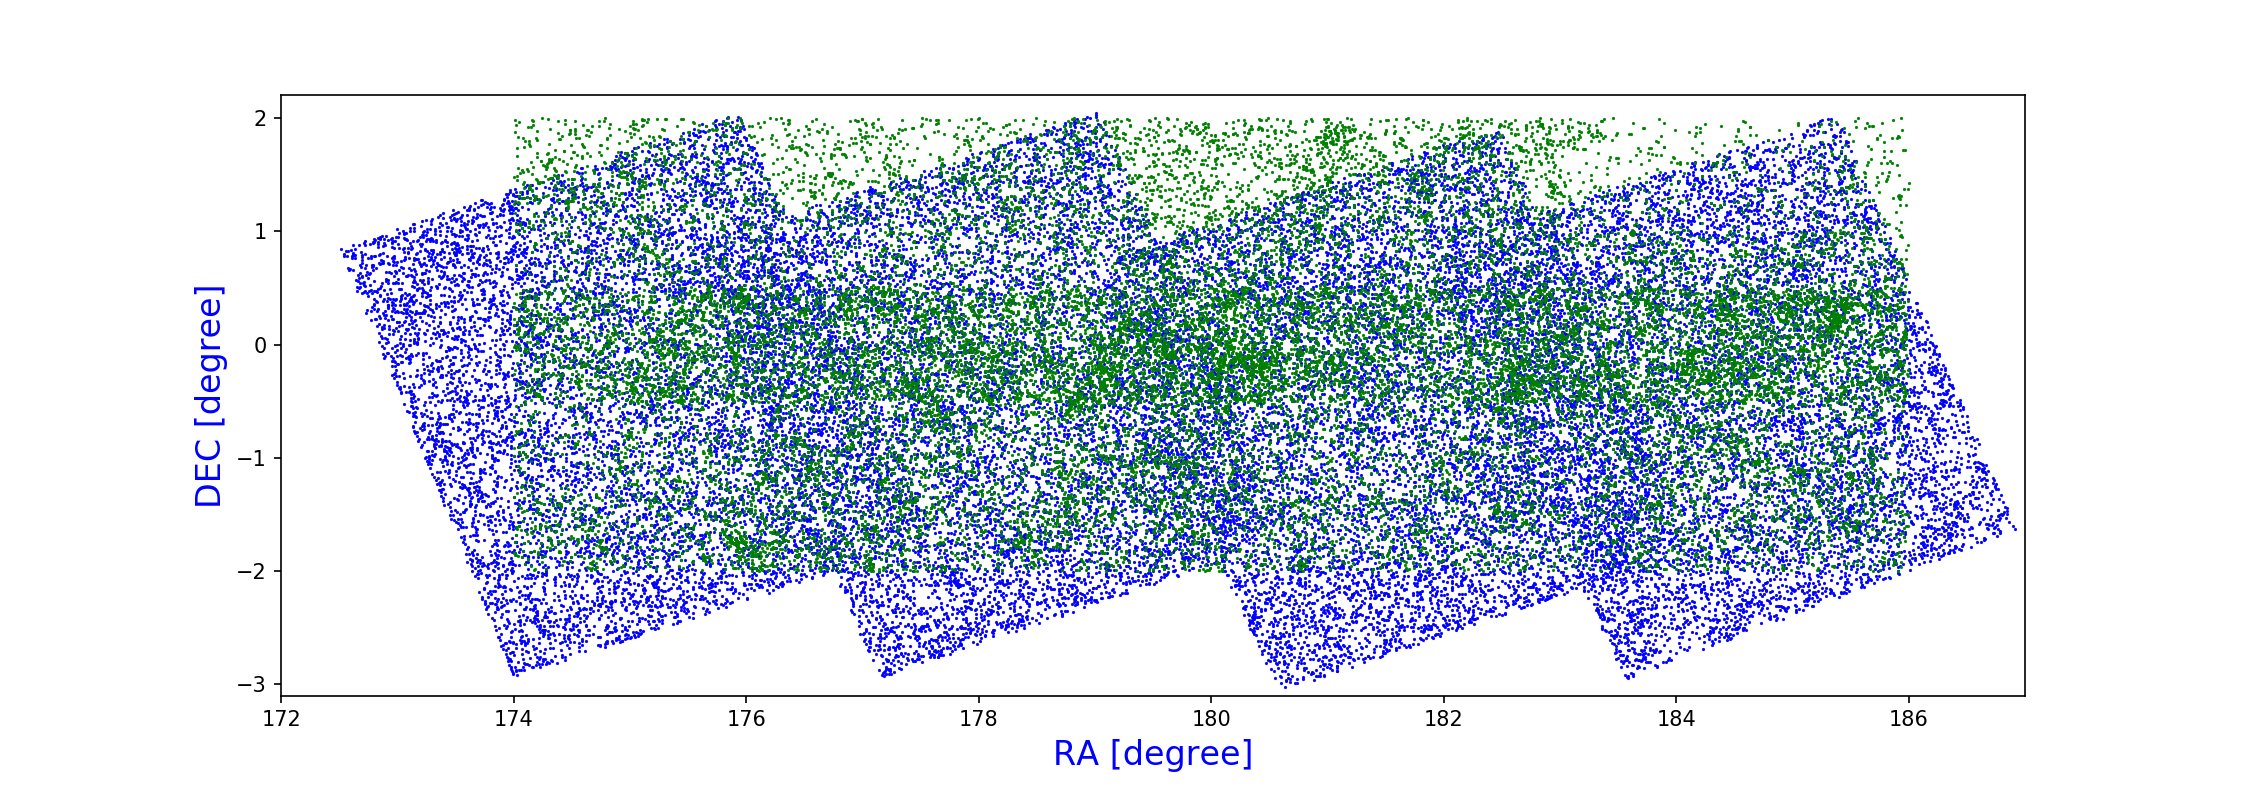
\includegraphics[width=\textwidth]{2_Muestras/region_2.png}}
      \vspace*{-10mm}
      \caption*{\small G12 (49.03 \maths{\mathrm{{deg}^{2}}}, verde) y Bloque 3  (54.40 \maths{\mathrm{{deg}^{2}}}, azul). Solapamiento: 43.46 \maths{\mathrm{{deg}^{2}}}.}
      
    \subfloat[]{
     \label{subfig:region_3}
      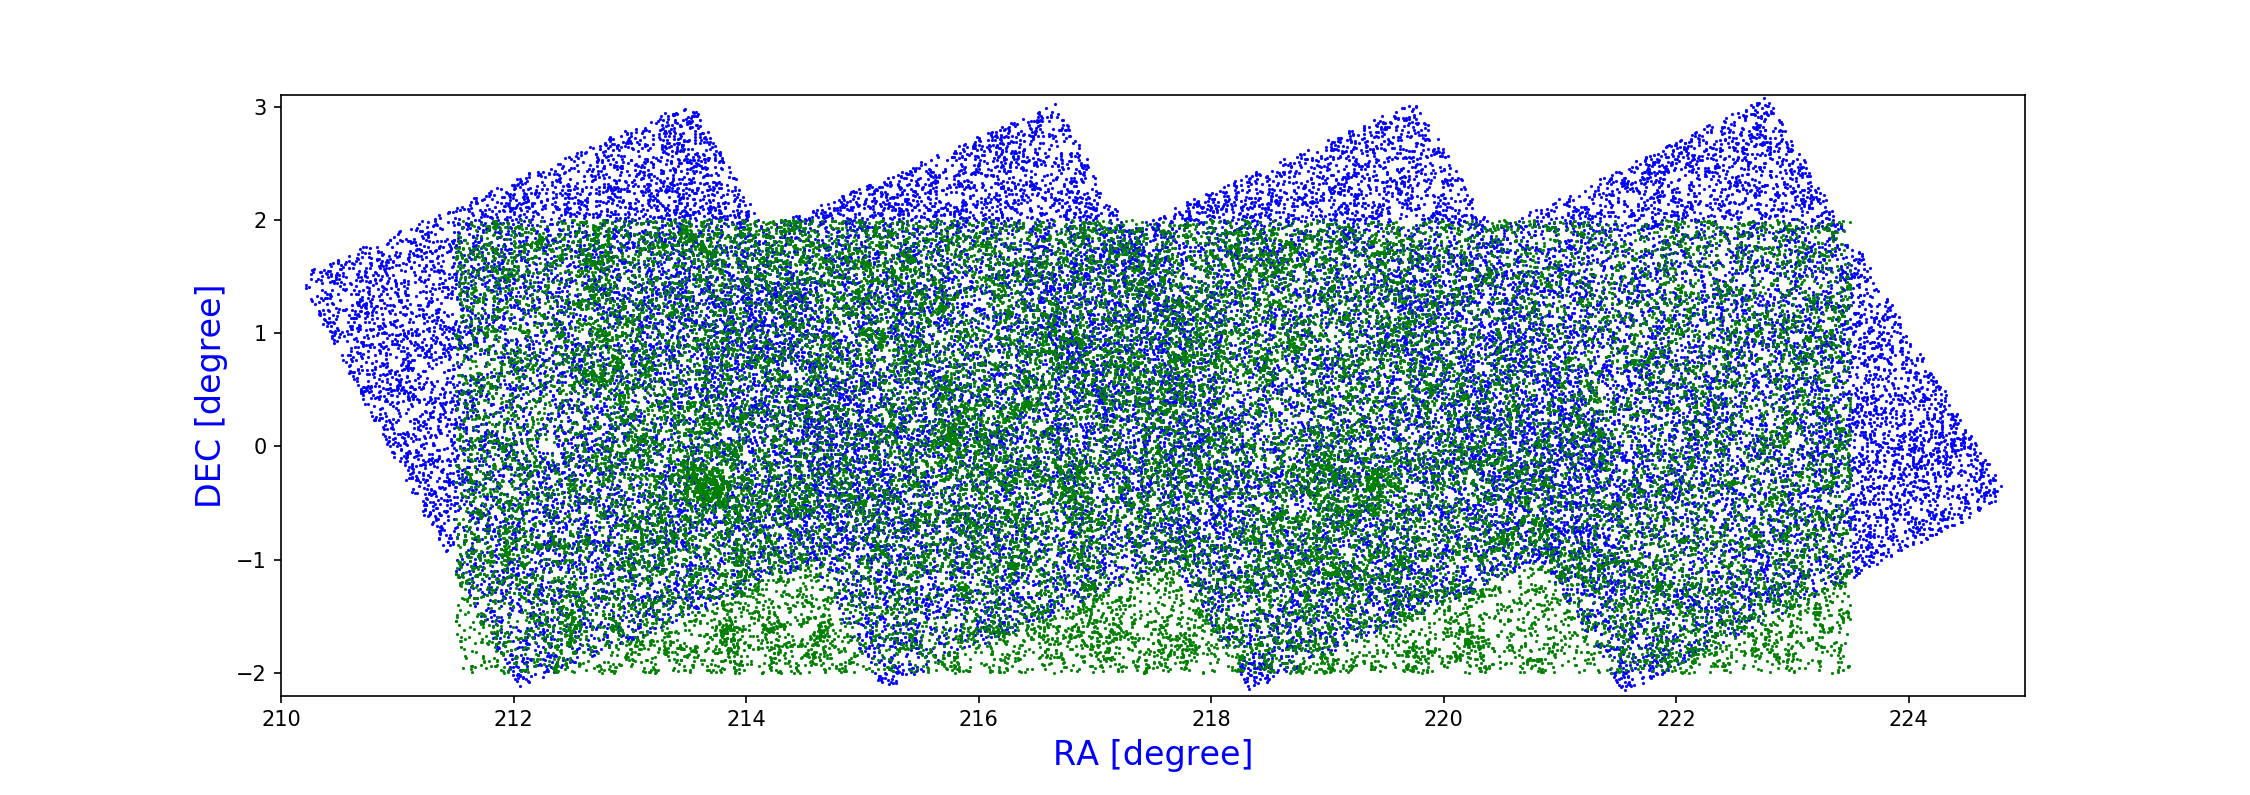
\includegraphics[width=\textwidth]{2_Muestras/region_3.png}}
      \vspace*{-10mm}
      \caption*{\small G15 (48.68 \maths{\mathrm{{deg}^{2}}}, verde) y Bloque 4 (54.80 \maths{\mathrm{{deg}^{2}}}, azul). Solapamiento: 43.88 \maths{\mathrm{{deg}^{2}}}.}
      
  \end{center}
  \caption{\small Superposición de los catálogos \gama\ (verde) y \hatlas\ (azul). Las áreas que se indican en el pie de cada imagen, se han obtenido a partir de la función \texttt{area\_region} que se encuentra definida en el Apéndice~\ref{apendice:codigo:get}. El área total cubierto por del catálogo \hatlas\ es de \maths{\sim163.35\;\mathrm{deg}^2} (según el proyecto \hatlas\ el área de los bloques 2, 3 y 4 es de \maths{161\;\mathrm{deg}^2}), el de \gama de \maths{\sim146.27\;\mathrm{deg}^2} (según \gama\ el área total de las tres regiones G09, G12 Y G15 es de \maths{144\;\mathrm{deg}^2}) y el área total de solapamiento de \maths{\sim130.3\;\mathrm{deg}^{2}}.}
  \label{fig:superposicion}
\end{figure}

\section{\anglicismo{Redshift} fotométrico de ETGs a partir de \spire}\label{sec:3_redshift_hatlas}

En esta sección se describe un método válido para estimar el \rt\ fotométrico de las ETGs a partir de las medidas del instrumento \spire\ del satélite espacial \h.  El método se basa en el hecho de que las ETGs poseen el máximo absoluto de emisión en el IR-lejano, sobre los \microm{100} para el sistema en reposo, debido a la emisión IR por parte del gas y polvo interestelar; dado que las medidas del \spire\ se encuentran a \microm{250}, \microm{350} y \microm{500}, estas coinciden en torno al máximo cuando \maths{1\lesssim z\lesssim3.5}. 

Se considera que a la emisión IR de las galaxias \anglicismo{starburst} contribuyen tres componentes diferentes, dependiendo del entorno astrofísico en que se originó: nubes moleculares, nubes difusas de baja densidad (cirros) y regiones circunucleares calentadas por el Núcleo Galáctico Activo (AGN) \citep{article:Lapi_2011}. De las tres, la componente \comillas{caliente}, procedente de las nubes de gas moleculares, es la que resulta relevante para el ajuste que se va llevar a cabo, debido a que es la componente más intensa en la zona del espectro en la que \spire\ realiza las medidas. En el rango de \maths{\lambda \sim 50-500\;\mu \mathrm{m}} (considerando el sistema en reposo), la SED de las galaxias \anglicismo{starburst} típicas puede modelarse (mostrando diferencias de entorno al \maths{10\%-20\%}) como suma de dos cuerpos grises\footnote{Puede encontrarse mucha más información sobre la ecuaciones del cuerpo gris en el artículo \cite{article:cuerpo_gris}.}  siendo el flujo \maths{{S}_{\nu}}, para cada uno de ellos, 

\begin{equation}
{S}_{\nu} \propto \frac{{\nu}^{3+\beta}}{\exp{\frac{h\nu}{K{T}_{d}}}-1},
\end{equation}

con temperaturas \maths{{T}_{d}\approx30\;\mathrm{K}} y \maths{{T}_{d}\approx60\;\mathrm{K}} y unos índices de emisividad para el polvo de \maths{\beta=1.7} y \maths{\beta=2} respectivamente. 
A diferencia de la mayoría de los algoritmos para determinar el \rt\ fotométrico, el método propuesto tomará como única referencia la SED de la galaxia \smm. Como veremos, esta decisión se fundamenta en los estudios realizados por \cite{article:Nuevo_2012} y \cite{article:Lapi_2011}. 

\subsection{Selección de la SED de referencia}\label{sec:selecion_sed} 

La idea de obtener el \rt\ fotométrico a partir de la SED de la galaxia \smm\ no es nuestra y las razones para elegir la SED de esta galaxia en concreto se explican con detalle en \cite{article:Lapi_2011}. Estos autores seleccionaron un conjunto de cuatro galaxias que consideraron representativas de las galaxias en formación típicas y cuya SED se encuentra bien determinada e hicieron varios estudios para saber cual era la SED más adecuada para realizar los ajustes. Para ello, en primer lugar identificaron las posibles fuentes de error a la hora de realizar el ajuste y consideraron que había dos fuentes de error principales.

La primera fuente de error está relacionada con el hecho de que resolución angular de los instrumentos de medida es menor cuanto mayor es la longitud de onda. Por este motivo la radiación electromagnética procedente de una fuente, tiende a mezclarse con la procedente de las fuentes próximas, lo cuál produce un incremento del flujo medido respecto del valor real. Para cuantificar el efecto que producen las fuentes débiles sobre las medidas del flujo llevaron a cabo simulaciones \cite{article:Rigby_2011} que muestran \porcentaje{56.5} de las fuentes detectadas a \maths{\geqslant\!5\;\sigma} a \microm{500} muestran un incremento en un factor \maths{>\!1.5}, y el \porcentaje{27.3} por un factor \maths{>\!2}, mientras que si la medida del flujo se encuentra por encima de los \maths{10\:\sigma}, el incremento de flujo debido a este fenómeno ya puede considerarse despreciable. Para saber cómo afecta el aumento de flujo sobre el cálculo del \rt\ fotométrico calcularon los \rts\ fotométricos de 39 galaxias, utilizado como referencia la \sed\ de cuatro galaxias diferentes, y lo compararon con el obtenido a partir de medidas espectroscópicas (Figura \ref{fig:redshift_comparacion}). Obtuvieron que el valor medio de la magnitud \maths{{\Delta z}/{(1+z)} \equiv {({z}_{\mathrm{phot}}-{z}_{\mathrm{spec}})}/{(1+{z}_{\mathrm{spec}})}} era menor cuando se utiliza la SED de \smm\ como modelo. 

\begin{figure}[htb]
    \begin{center}
         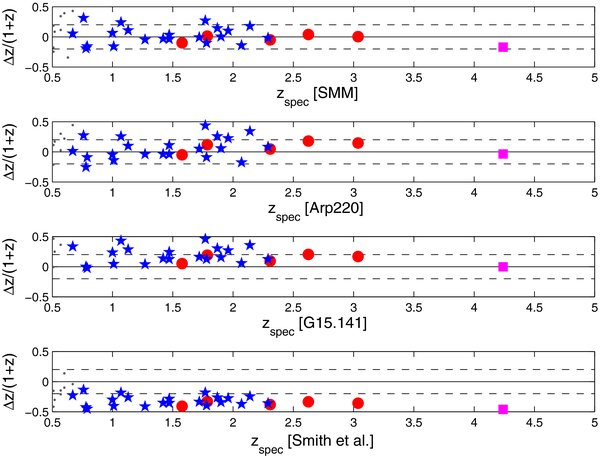
\includegraphics[width=14cm]{3_Redshift_Hatlas/apj404107f3_lr.jpg}
    \end{center}
    \vspace{-5mm}
    \caption{\small Comparación del \rt\ espectroscópico con el \rt\ fotométrico obtenido mediante el ajuste por mínimos tomando como referencia cuatro SEDs diferentes. Figura extraída del artículo \cite{article:Lapi_2011}.} 
    \label{fig:redshift_comparacion}
\end{figure}

Otra posible causa de error en la estimación del \rt\ proviene de la gran variedad de las galaxias con una tasas de formación estelar elevadas. Para estudiar cómo afecta la diversidad de galaxias en la estimación del \rt\ generaron una muestra de \maths{9\times{10}^{3}} galaxias a las que asignaron aleatoriamente un \rt\ comprendido entre \maths{1\geqslant\!z\!\geqslant 3.5} y una \sed\ procedente de un conjunto de 19 galaxias con una \sed\ bien conocida, todas ellas con una \sfr s \maths{\geqslant\,}\tfe{20} y una contribución del núcleo galáctico activo al flujo en el IR-Lejano inferior al \porcentaje{10} (a los \comillas{flujos simulados} de \microm{250}, \microm{350} y \microm{500} se les asignaron errores de forma aleatoria a partir de errores procedentes de observaciones reales). 
El siguiente paso fue calcular el \rt\ fotométrico de la muestra simulada utilizando como referencia la \sed\ de las galaxias \arp, \gquince\ y \smm. Después, corrigieron los valores del \rt\ fotométrico a partir de las desviaciones medias obtenidas en el estudio anterior y realizaron el histograma de la Figura \ref{fig:sed_distrib_simulacion}, reconociendo que la distribución de los \rts\ obtenidos solo se ve moderadamente afectada por la elección de la SED.

\begin{figure}[htb]
    \begin{center}
         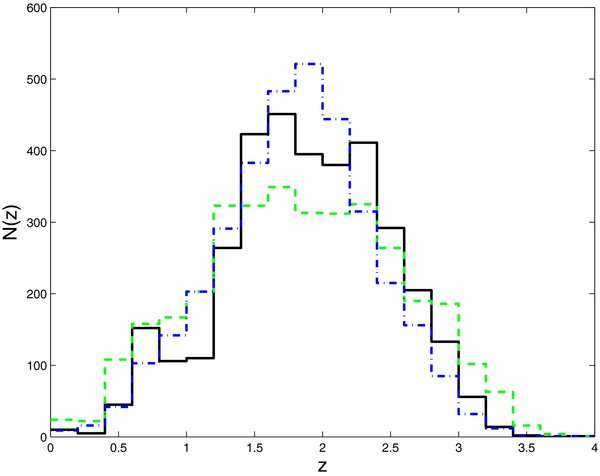
\includegraphics[width=14cm]{3_Redshift_Hatlas/simulacion_rt_distribution.jpg}
    \end{center}
    \vspace{-5mm}
    \caption{\small Distribución del \rt\ fotométrico, para las fuentes de la muestra con \maths{9\times{10}^{3}} galaxias simuladas, tomando como referencia la SED \smm\ (curva negra continua), tomando como referencia la SED de la galaxia Arp 220 (curva discontinua verde) y la SED de la galaxia G15.141 (curva discontinua azul). La figura pertenece al artículo \cite{article:Lapi_2011}.}
    \label{fig:sed_distrib_simulacion}
\end{figure}

A partir de estos estudios concluyeron que, si bien los \rt\ obtenidos son muy parecidos independientemente del modelo que tomemos como referencia (cualquiera de los considerados), la SED de la galaxia \smm\ resulta la más adecuada para realizar los ajustes. 

\newpage
\subsubsection{La galaxia \smm.}
La galaxia \smm\ ha sido cuidadosamente estudiada y se dispone de información detallada sobre ella. Como nos explican en \cite{article:smmj} se trata de una galaxia que muestra un \rt\ \maths{z=2.3259\pm0.0001} y que ha sido gravitatoriamente magnificada un factor \maths{\mu=32.5\pm4.5} por un grupo de galaxias con z=0.325. Es una galaxia especialmente brillante en el infrarrojo, con un flujo \flujo{870}=\mjy{\:106.0\,\pm\,7.0}. Su tasa de formación estelar es \sfr~=~\tfe{210\;\pm\;50} y se estima que la cantidad de materia bariónica es de \masassolares{M_{bar}=(4\pm2)\times{10}^{10}} siendo \maths{\sim 75\%} masa estelar y el resto gas y polvo. 

En la Figura \ref{fig:sed_lambda} se muestra la representación de la radiancia espectral (normalizada a \maths{5570}~\AA) \maths{S_{\lambda}} de la galaxia a partir de la interpolación lineal de los puntos del fichero que utilizamos como referencia. 
El máximo de emisión en el IR-lejano puede observase sobre los \maths{10^{6}}~\AA~\maths{\equiv 100\:\mu \mathrm{m}} (el máximo se aprecia mejor en la representación \maths{S_{\nu}}, Figura \ref{fig:sed_nu}).
Esta no es un curva obtenida de forma completamente experimental; se parte de un conjunto de puntos reducido (del orden de una decena) y después a partir de modelos teóricos\footnote{En \cite{article:Nuevo_2012} y \cite{article:Lapi_2011} se indica que las SEDs que ellos utilizan han sido modeladas utilizando el código GRASIL.}, se obtienen el resto de puntos de la curva que vemos. La zona \maths{\lambda \sim 50-500\;\mu \mathrm{m}} se modela a partir de las ecuaciones del cuerpo gris.
En realidad, el hecho de que los valores de los \rts\ obtenidos solo se vean moderadamente afectados por la elección de la SED, se debe en gran medida a que la información de la que se dispone de todas las galaxias consideradas como posible referencia en la Sección \ref{sec:selecion_sed} es limitada en esa zona del espectro\linebreak y cuando se modela la SED de cada una de ellas el resultado es parecido en todos los casos.

\begin{figure}[htb]
    \begin{center}
         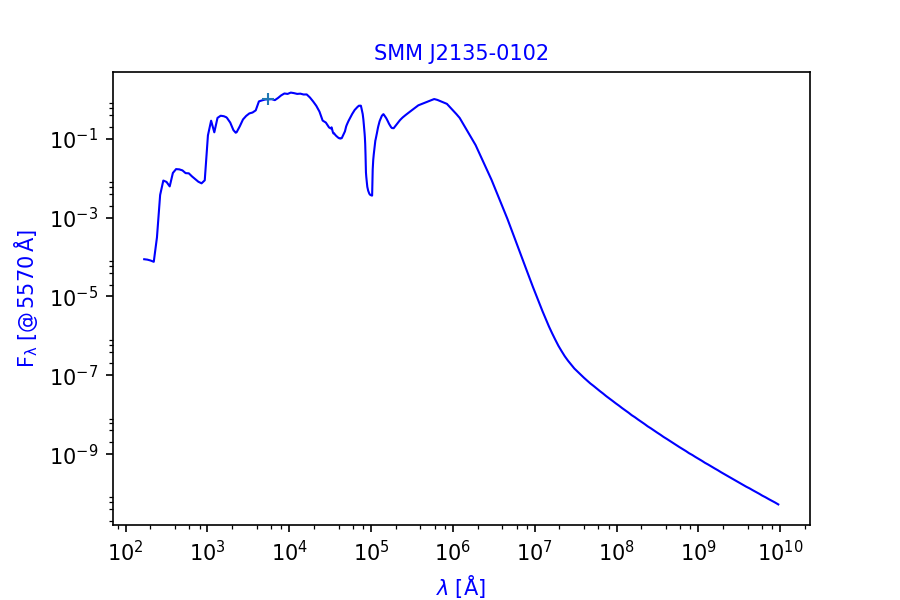
\includegraphics[width=14cm]{3_Redshift_Hatlas/grafica_SMM_F_lambda.png}
    \end{center}
    \vspace{-5mm}
    \caption{\small Representación en escala logarítmica del flujo \maths{F_{\lambda}} de la galaxia \smm\ normalizado a \angstrom{5570}. El punto en el que se encuentra el símbolo \maths{+} indica el punto de normalización.}
    \label{fig:sed_lambda}
\end{figure}

% Como se obtiene la sed se puede ver en Lapi et al(2011) pag 5
\newpage
\subsection{Algoritmo}

El \rt\ se obtiene mediante un ajuste de mínimos \maths{{\chi}^{2}} de la \sed\ normalizada de la galaxia \smm\ a los tres puntos experimentales proporcionados por el instrumento \spire. 
La \sed\ de la galaxia modelo se obtiene a partir de un fichero con dos columnas; la primera contiene los valores de la longitud de onda en \AA, la segunda los valores la densidad espectral de flujo\footnote{La SWIRE \anglicismo{Template Library} contiene la SED de 25 galaxias que se pueden utilizar como modelo: \url{http://www.iasf-milano.inaf.it/~polletta/templates/swire_templates.html}. La SED de la galaxia \smm\ ("The Cosmic Eyelash") que se utiliza en este trabajo, no se encuentra en esa librería, pero sigue la misma normalización.} \maths{F_{\lambda}}, normalizado a \angstrom{5570}. El flujo expresado en unidades de \maths{F_{\lambda}} tiene dimensiones de \maths{\mathrm{[M\,{L}^{-1}\,{T}^{-3} ]}}, sin embargo las medidas del \spire\ se encuentran en \jy{}, que es una unidad de \maths{F_{\nu}} con dimensiones de \maths{\mathrm{[M \,{T}^{-2} }]}. Para pasar de una unidad a la otra es suficiente tener en cuenta la relación \maths{|F_{\lambda}\mathrm{d}\lambda|=|F_{\nu}\mathrm{d}\nu|} . Los valores del flujo espectral que no se encuentran en el fichero se obtienen mediante interpolación lineal.

Para realizar el ajuste se tomarán dos parámetros, que denominaremos \paramc\ y \paramk. La curva de ajuste se obtiene multiplicando los valores del flujo por \paramc\ y los valores de la longitud de onda por \paramk.
En el sentido matemático, el ajuste consiste en una dilatación (o contracción) de la \sed\ de referencia en la dirección de cada uno de los ejes de coordenadas.

En el sentido físico la dilatación el en el eje \maths{y} podría interpretarse como un factor que indica cómo de luminosa es la galaxia considerada respecto de la galaxia de referencia. Sin embargo, la curva de referencia que se ha utilizado, está normalizada para un valor concreto de \maths{\lambda} por lo que no conocemos cuáles son las unidades físicas. Nos serviría para comparar magnitudes relativas entre los objetos del catálogo.
La dilatación en \maths{\lambda} se corresponde con un desplazamiento al rojo del espectro electromagnético con respecto a la \sed\ de referencia. Para entender cómo se relaciona el parámetro de ajuste \paramk\ con el \rt, \z, podemos verlo del siguiente modo:  Dado que la \sed\ de referencia no tiene \rt\ puesto que se supone que es la \sed\ de la galaxia \smm\ en un sistema en reposo (también habiendo corrigiendo el \rt\ debido al corrimiento al rojo cosmológico), esta curva nos daría la longitud de onda de emisión, \maths{{\lambda}_{e}}. La longitud de onda que observada\footnote{El nombre desplazamiento al rojo sugiere inmediatamente la posibilidad de realizar un ajuste mediante un \comillas{desplazamiento} de la \sed\ de referencia sobre el eje \maths{x}, sin embargo esto carece de sentido físico. Si en vez de multiplicar por \paramk\ consideramos una traslación del tipo \maths{{\lambda}_{o}={\lambda}_{e} + K} y sustituimos en la Ecuación \ref{eq:z_general} obtendremos

\begin{equation*}
 z = \frac{{\lambda}_{o} - {\lambda}_{e}}{{\lambda}_{e}} = \frac{{\lambda}_{o} - ({\lambda}_{o} + K) }{ {\lambda}_{o} + K } .
\end{equation*}

Esto no puede ser, porque obtendríamos un \rt\ diferente dependiendo de qué valor de \maths{\lambda} estuviésemos midiendo. 

} se corresponderá con la obtenida a partir del ajuste, es decir, \maths{{\lambda}_{o}={\lambda}_{e} \times K}, por tanto, utilizando la definición general de corrimiento al rojo,

\begin{equation*}
 z = \frac{{\lambda}_{o} - {\lambda}_{e}}{{\lambda}_{e}} = \frac{{\lambda}_{o} - \frac{{\lambda}_{o}}{K} }{ \frac{{\lambda}_{o}}{K} } = \frac{ ({\lambda}_{o} \times K) - {\lambda}_{o}}{{\lambda}_{o}} = K - 1.
\end{equation*}

La función del programa escrito en \python\ hace uso de esta relación para calcular \z.

\begin{figure}[htb]
    \begin{center}
         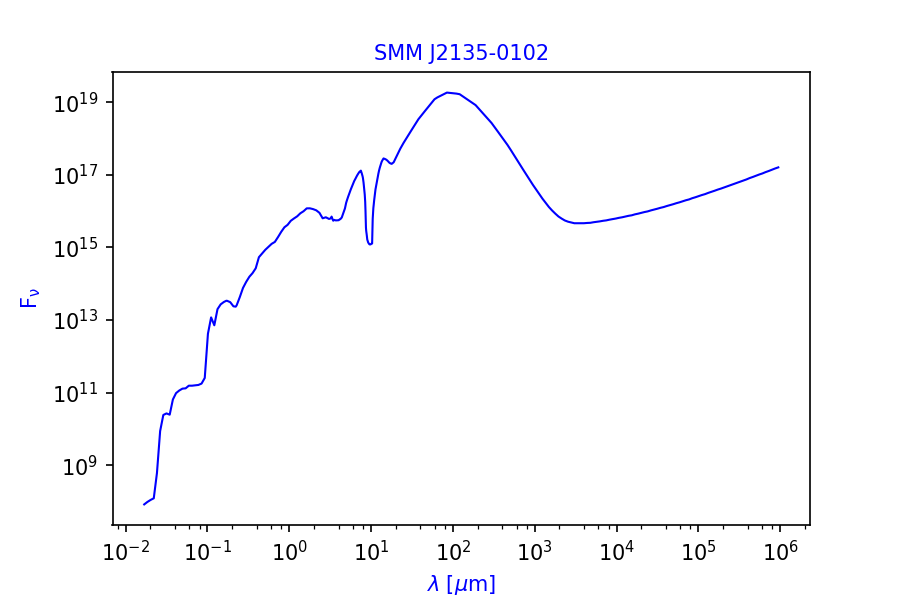
\includegraphics[width=14cm]{3_Redshift_Hatlas/grafica_SMM_F_nu.png}
    \end{center}
    \vspace{-5mm}
    \caption{\small \sed\ de la galaxia \smm. A diferencia de la Figura~\ref{fig:sed_lambda}, en este caso se está representando \maths{F_{\nu}} en vez de \maths{F_{\lambda}}. Esta curva es la que se utilizará como referencia para los ajustes. La zona \maths{\lambda \sim 50-500\;\mu \mathrm{m}} ha sido modelada como suma de dos cuerpos grises con temperaturas \maths{{T}_{d}\approx30\;\mathrm{K}} y \maths{{T}_{d}\approx60\;\mathrm{K}} y unos índices de emisividad para el polvo de \maths{\beta=1.7} y \maths{\beta=2} respectivamente.}
    \label{fig:sed_nu}
\end{figure}

\begin{figure}[H]
  \begin{center} 
  
    \subfloat[]{
     \label{subfig:ajuste_a}
      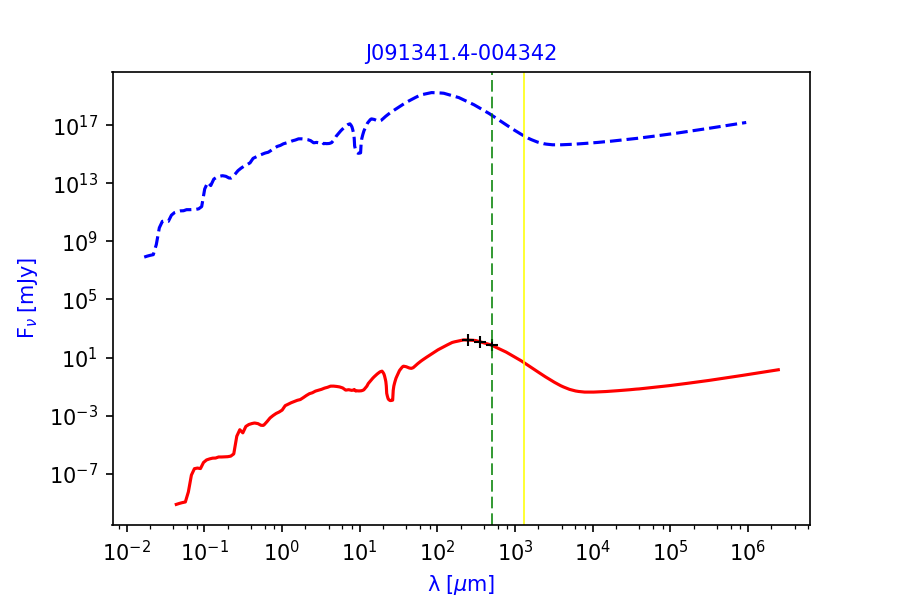
\includegraphics[width=0.8\textwidth]{3_Redshift_Hatlas/ajuste_6.png}} 
      
    \subfloat[]{
     \label{subfig:ajuste_b}
      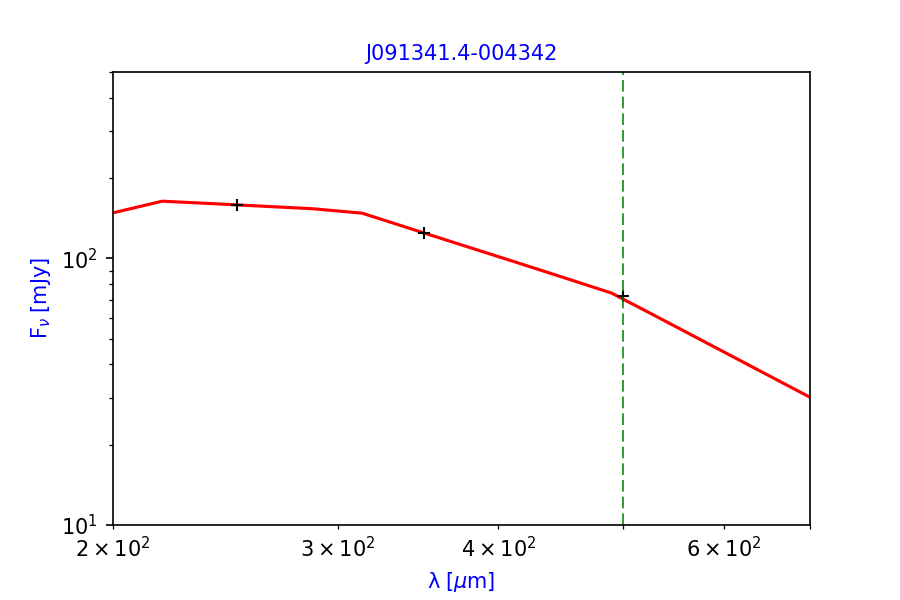
\includegraphics[width=0.8\textwidth]{3_Redshift_Hatlas/ajuste_6_zoom.png}}

  \end{center}
    
  \caption{\small Ajuste por mínimos cuadrados de la SED de la galaxia \smm\ para el objeto J091341.4-004342 del catálogo \hatlas. En la figura \ref{subfig:ajuste_a}, la curva discontinua es la curva mostrada en la Figura \ref{fig:sed_nu}. La curva continua es la curva del ajuste, que se encuentra sobre los tres puntos experimentales de un objeto, que vienen representados por el símbolo '+'. Al utilizar la representación logarítmica, en cada uno de los ejes, la curva roja aparenta ser un desplazamiento de la curva azul. Las líneas verticales se utilizan para visualizar el desplazamiento horizontal relacionado con el desplazamiento al rojo \z. En el caso del eje~\maths{x} el desplazamiento será \maths{\log_{10}{(z+1)}}. En la figura \ref{subfig:ajuste_b} se muestra con más detalle la zona de encuentro de la curva de ajuste con los puntos experimentales. Se aprecia perfectamente que la curva roja se compone de segmentos unidos, debido a que solo conocemos un conjunto de \maths{\sim1000} valores de la \sed\, el resto se obtiene mediante interpolación lineal a partir de estos.}
\end{figure}

\subsection{Confrontación del método}

Cabe señalar que en este trabajo no se ha probado que el método descrito en esta sección proporcione ajustes válidos para obtener el \rt\ fotométrico de las ETGs. Para hacer eso, deberíamos disponer de una muestra suficientemente grande de fuentes con \rt\ espectroscópico para poder comparar los valores obtenidos con una referencia fiable. Aunque no disponemos de esa información, en el artículo~\cite{article:Nuevo_2012} se ha publicado una tabla con el valor del \rt\ de 64 galaxias que ellos calcularon utilizando su propio programa. En la Figura~\ref{fig:redshift_comparacion} se ha hecho un ajuste para comparar sus resultados con los nuestros.  

\vspace*{-15mm}

\begin{figure}[h]
    \begin{center}
         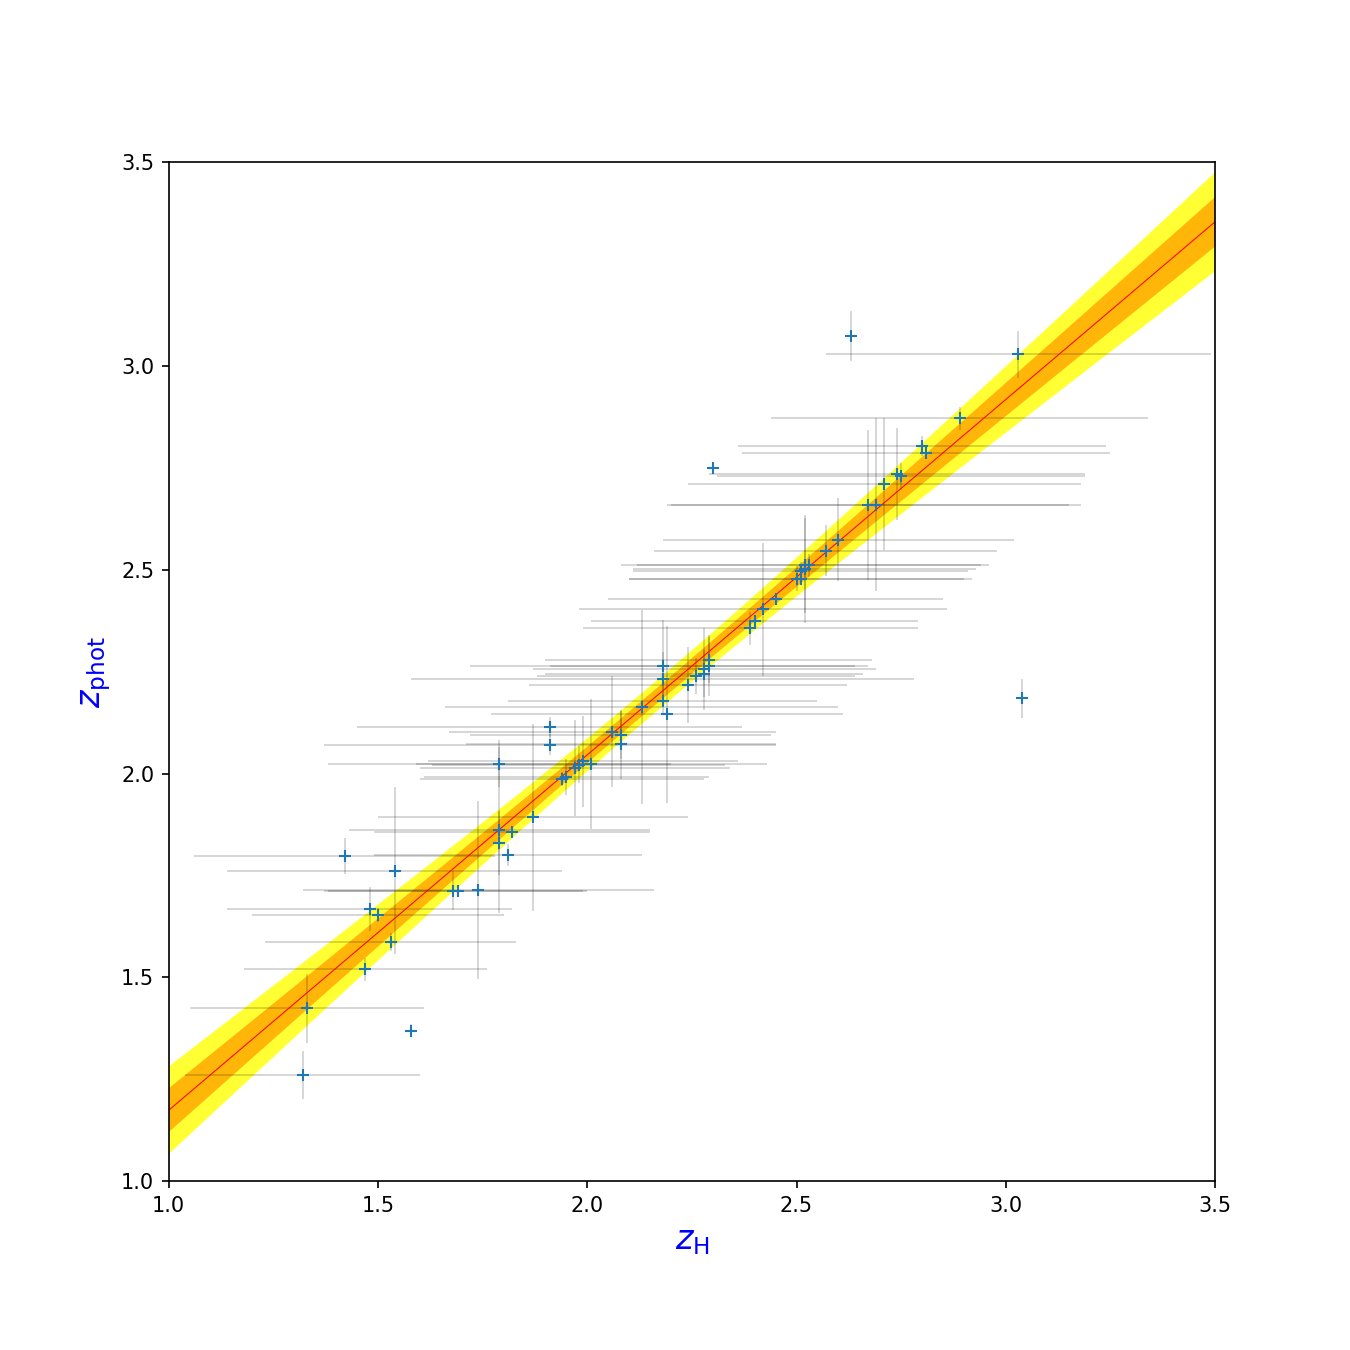
\includegraphics[width=16cm]{3_Redshift_Hatlas/comparacion_Z.png}
    \end{center}
    \vspace*{-15mm}
    \caption{\small Comparación del \rt\ fotométrico obtenido utilizando el algoritmo descrito en la Sección~\ref{sec:3_redshift_hatlas}, \maths{z_{\mathrm{phot}}}, con los valores del \rt\ fotométrico estimado por \cite{article:Nuevo_2012}, \maths{z_{\mathrm{H}}}. La linea roja representa el ajuste lineal, \maths{{z}_{\mathrm{phot}}=(0.87 \pm 0.04)\times {z}_{\mathrm{H}}+(0.3 \pm 0.1)}. La zona anaranjada representa la zona con una confianza \maths{\sigma<1} y la amarillenta \maths{\sigma<2}. Las barras de error no se han tenido en cuenta para realizar el ajuste. Las barras de error horizontales se corresponden los los valores asignados a las medidas que aparecen en el artículo, las barras de error verticales se obtienen a partir de la varianza del ajuste proporcionado por el programa que aparece en la Sección \ref{apendice:codigo:rojo} (Los valores utilizados para realizar la gráfica se encuentran en la Tabla~\ref{tab:redshift_halos}).} 
    \label{fig:comparacion_sed}
\end{figure}

La tabla del artículo no solo proporciona los valores del \rt\ fotométrico que ellos obtuvieron, también los valores de la desviación estándar que ellos asignaron a estas medidas. Al no disponer de una muestra de referencia con la que realizar estudios estadísticos, tampoco disponemos de los recursos suficientes para asignar valores a \maths{\sigma^z}. Para asignar los valores de \maths{{\sigma}^z} a los \linebreak
\\
valores \maths{z_{\mathrm{phot}}} obtenidos mediante nuestro método, se ha realizado un ajuste similar al mostrado en la Figura~\ref{fig:ajuste_error_gama}, partiendo de las desviaciones estándar asignadas a los desplazamientos al rojo del ajuste realizado en el artículo (Figura~\ref{fig:ajuste_errores_ajuste}).

\vspace*{-1mm}

\begin{figure}[h]
    \begin{center}
         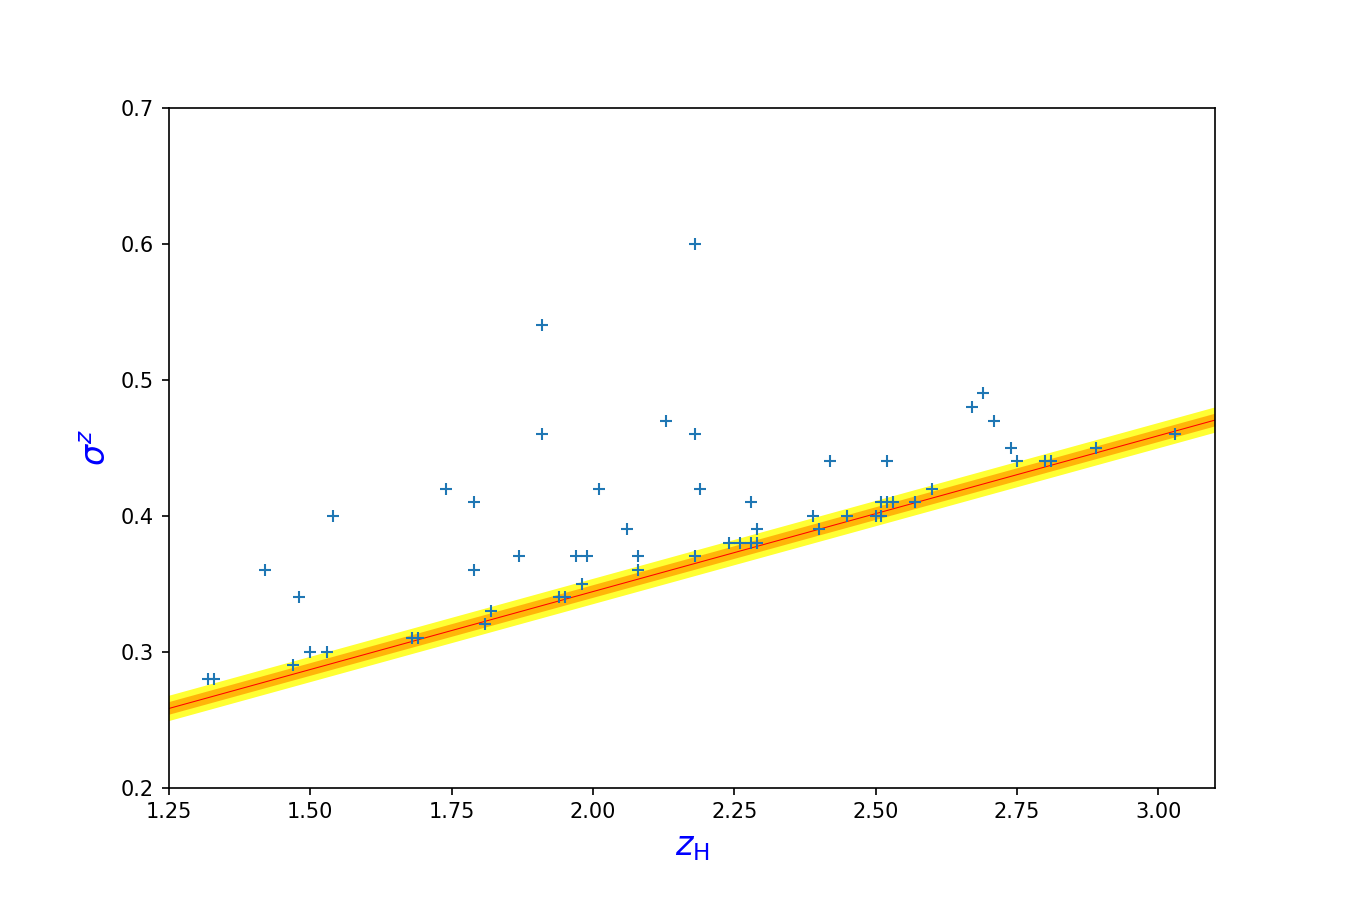
\includegraphics[width=16cm]{3_Redshift_Hatlas/ajuste_errores.png}
    \end{center}
    \vspace*{-10mm}
    \caption{\small Representación de la desviación estándar del \rt, \maths{{\sigma}^{z}} en función de \maths{z_{\mathrm{H}}}. Los valores de los puntos representados se encuentran en la Tabla~\ref{tab:redshift_halos}. La recta se ha obtenido mediante un ajuste lineal de la forma \maths{{\sigma}^z= a\times(1+z)} con \maths{a} como parámetro de libre. El parámetro resultante del ajuste ha sido \maths{a=0.115\pm 0.005}.}
    \label{fig:ajuste_errores_ajuste}
\end{figure}


\vspace*{-1mm}




\section{Método probabílistico de Cross-Identificación}\label{sec:4_cross_identificacion}

Los métodos de \cross\ son herramientas que proporcionan criterios estadísticos para determinar cuando observaciones pertenecientes a catálogos diferentes pertenecen a un mismo objeto astronómico o a varios. Son especialmente útiles porque facilitan el estudio de los objetos astronómicos en múltiples longitudes de onda; dado que no es posible estudiar un objeto en múltiples longitudes de onda con un único instrumento, se hace necesario acudir a algoritmos que automaticen la tarea de identificar las observaciones de un conjunto de objetos en distintos cartografiados. Cuando los cartografiados cuentan con cientos de miles de observaciones esta tarea resulta imposible de realizar de otro modo. 

El criterio de \cross\ que nosotros proponemos se sirve dos factores de Bayes; un factor de Bayes posicional y otro fotométrico propuestos por Tamás Budavári y Alexander S. Szalay. Partiremos de dos hipótesis mutuamente excluyentes; en adelante \maths{H_1} es la hipótesis de que los emparejados considerados están formados por observaciones de un mismo objeto astronómico y \maths{H_2} la hipótesis de que se trata de observaciones pertenecientes a dos objetos diferentes. El factor de Bayes que nos permitirá discernir entre ambas hipótesis será,

\vspace{-3mm}

\begin{equation}
    B_{12}= B^{p}_{12}\times B^{z}_{12}
\end{equation}

llamado factor de Bayes conjunto, obtenido como producto del factor de Bayes posicional \maths{B^{p}_{12}} y el factor de Bayes fotométrico \maths{B^{z}_{12}}. Los objetos cuyo valor \maths{B_{12}>1} son las contrapartidas formadas por observaciones de un mismo objeto en los dos catálogos. Para estar seguros de que esto es así, es conveniente que el factor de Bayes posicional sea mucho mayor que 1 (ver criterio de Harold Jeffreys: Tabla~\ref{tab:bayes_interpretacion})

El criterio de \cross\ será tanto mejor cuanto mayor sea la resolución espacial de los catálogos utilizados y menores sean los errores de la medida del \rt. Todas las observaciones pertenecientes a un mismo catálogo tienen el mismo error posicional (para los catálogos considerados). Esto va dar lugar a una distancia angular \maths{\sim50\:\mathrm{arcsec}} por debajo de la cual dos observaciones son siempre consideradas como pertenecientes a un mismo objeto teniendo en cuenta únicamente el factor de Bayes posicional (este límite lo marca el valor \maths{B^{p}_{12}=1}, ver Figura~\ref{fig:bayes_posicional}). 
El caso del criterio fotométrico es diferente y no existirá algo como una diferencia umbral entre \rt s; las medidas del \rt\ de cada observación en cada uno de los catálogos tiene un error diferente, por lo cual la casuística es mucho más variada (Figura~\ref{fig:bayes_fotométrico}). 

La representación de los factores de Bayes de los emparejamientos encontrados que se muestra a continuación es importante para entender posteriormente cuales son los límites de nuestro método para la identificación de SLGs teniendo en cuenta las desviaciones estándar de las medidas de las que disponemos.
Las dos secciones que siguientes se dedican a describir cómo obtuvieron los autores citados anteriormente el factor de Bayes posicional y fotométrico.

\newpage

\begin{figure}[H]
    \begin{center}
         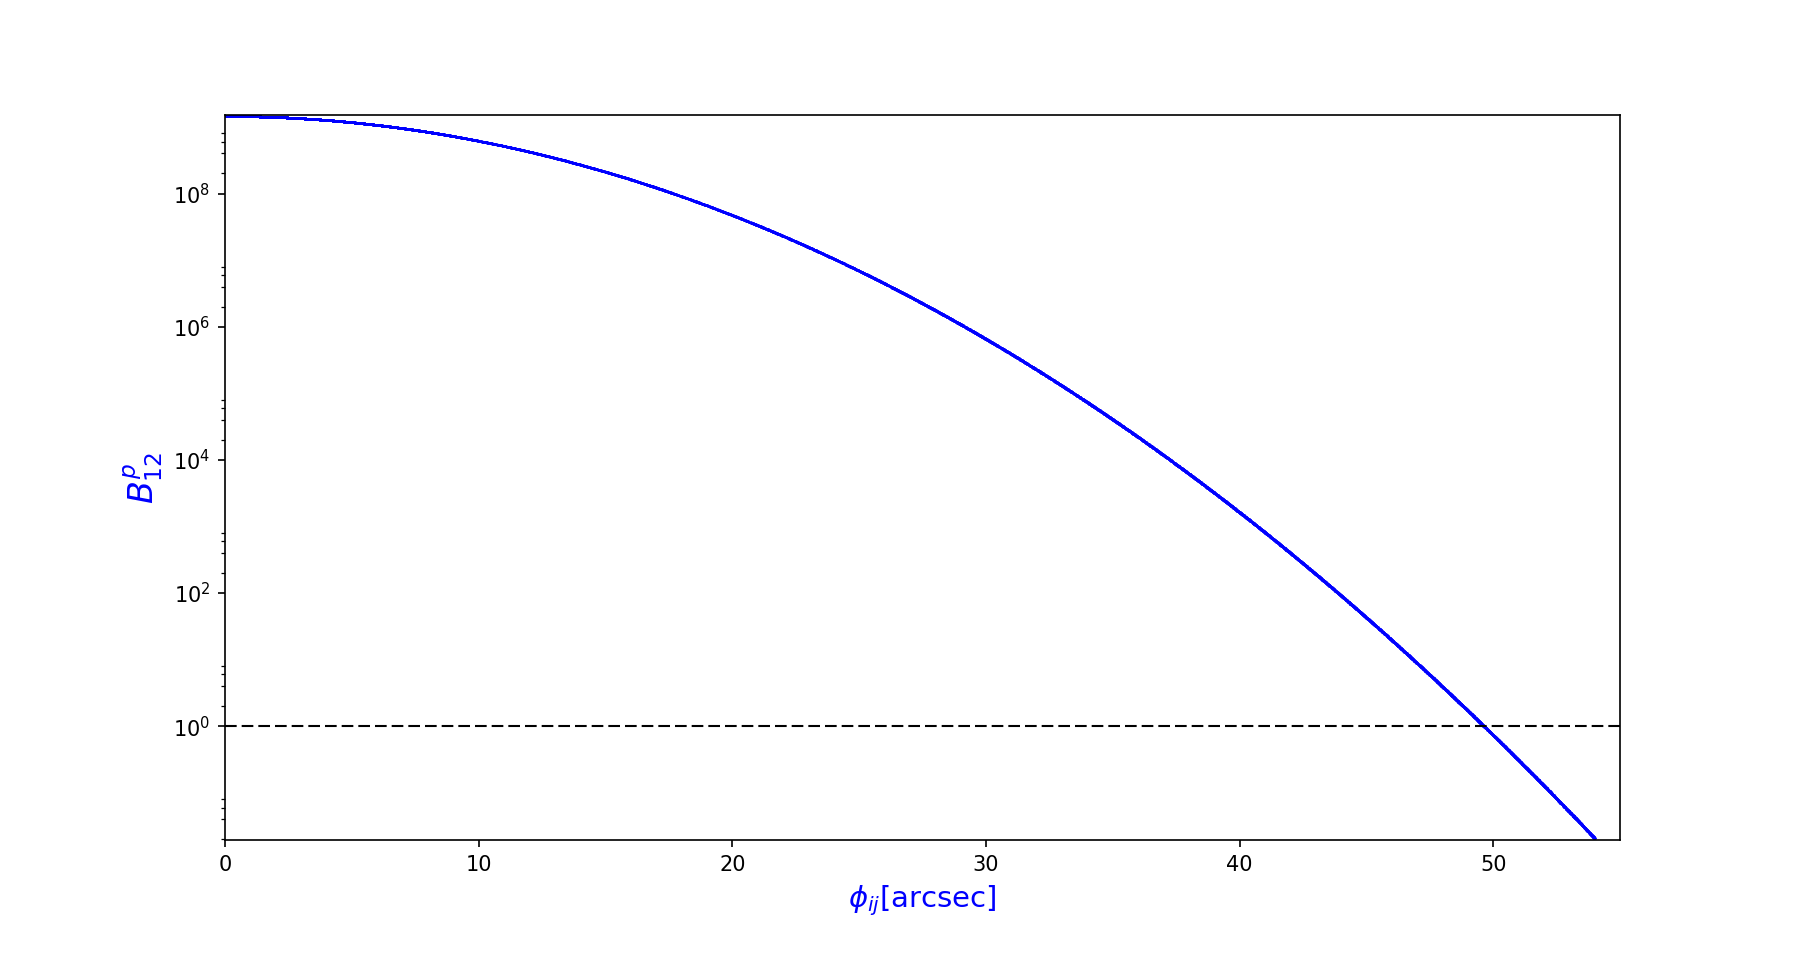
\includegraphics[width=\textwidth]{4_cross_identificacion/matching_ghbayes_posmatching_gh.png}
    \end{center}
    \vspace*{-10mm}
    \caption{\small Representación del factor de Bayes posicional en función de la distancia angular para las contrapartidas formadas por observaciones pertenecientes a \hatlas\ que se encuentran a una distancia angular inferior a \maths{54\:\mathrm{arcsec}} de otra perteneciente a \gama. La línea horizontal discontinua separa las contrapartidas con valores \maths{B^{p}_{12}<1} y \maths{B^{p}_{12}>1}. Considerando los valores de los errores instrumentales del catálogo \gama, \maths{\sigma_g^{p}\simeq0.297\;\mathrm{arcsec}} y del catálogo \hatlas,  \maths{\sigma_h^{p}\simeq7.63\;\mathrm{arcsec}}, el valor máximo que puede tomar \maths{B^{p}_{12}~\!\!~=~\!\!~9~\times~10^{9}} y la separación angular para la cual \maths{B^{p}_{12}=1} es \maths{\phi_{12}\sim49.64\:\mathrm{arcsec}}.}
    \label{fig:bayes_posicional}
\end{figure}

\vspace{-5mm}

\begin{figure}[H]
    \begin{center}
         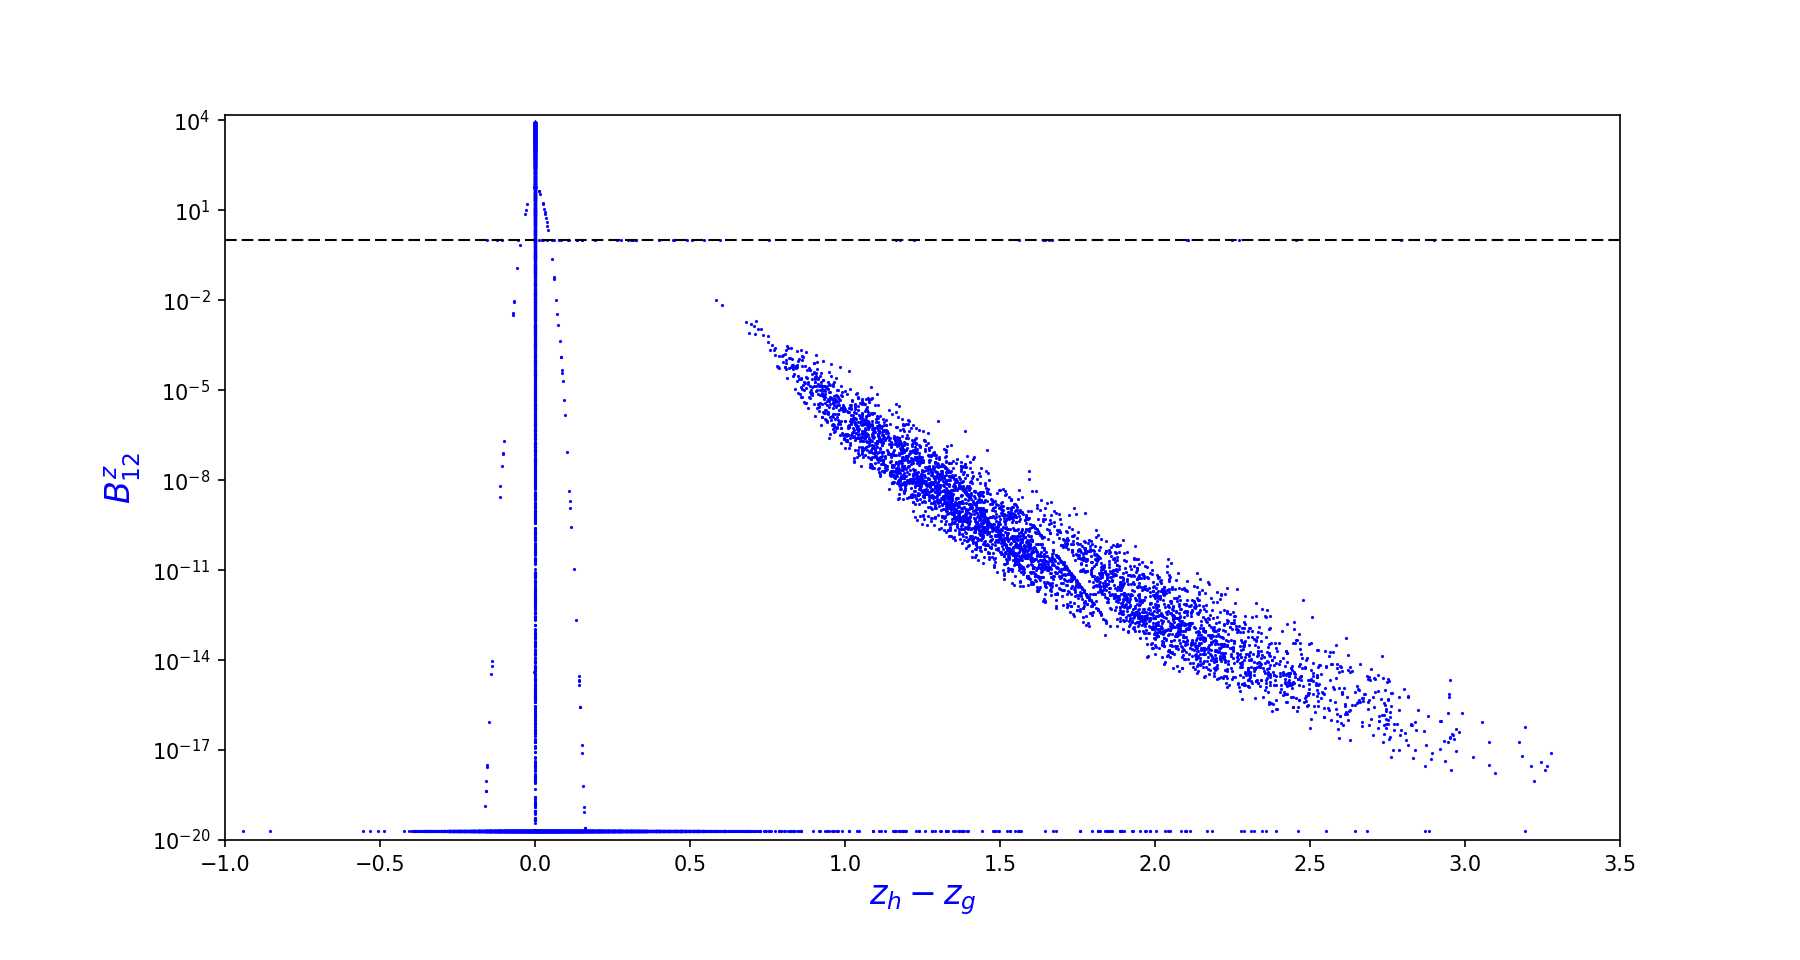
\includegraphics[width=\textwidth]{4_cross_identificacion/matching_ghbayes_zmatching_gh.png}
    \end{center}
    \vspace*{-10mm}
    \caption{\small Representación del factor de Bayes fotométrico en función de la diferencia entre los \rt\ de los catálogos \hatlas\ y \gama,  \maths{z_h-z_g}, para todas las contrapartidas formadas por observaciones de \hatlas\ que se encuentran a una distancia angular inferior a \maths{54\:\mathrm{arcsec}} de otra de \gama\ tomando \maths{z_{max}=3.5}. La línea discontinua horizontal marca el límite entre los puntos con valores \maths{B^{z}_{12}<1} y \maths{B^{z}_{12}>1}. En este caso, a diferencia del factor de Bayes posicional, cada medida del \rt\ tiene su propio valor del error, por lo que al realizar la representación los puntos aparecen como una nube de puntos. El valor máximo que puede tomar el factor de Bayes espectroscópico es \maths{B^{z}_{12}=8462} considerando \maths{z_h-z_g=0} y \maths{\sigma^z=1.1\times{10}^{-4}} para las dos observaciones que forman el pareo.}
    \label{fig:bayes_fotométrico}
\end{figure}


\subsection{Factor de Bayes posicional propuesto por Budavári \& Szalay}\label{sec:bayes_posicional}

Estos autores modelizan la posición verdadera de un objeto sobre la esfera celeste mediante un vector tridimensional unitario \maths{\boldsymbol{m}} y las posiciones observadas del mismo a partir del conjunto de vectores unitarios  \maths{D=\{\boldsymbol{x}_1,\boldsymbol{x}_2\ldots \boldsymbol{x}_n\}}. 
Debido a que hay un error instrumental, no podemos afirmar que la medida sobre la posición de un objeto, \maths{{\boldsymbol{x}}_i}, se corresponda exactamente con su posición verdadera \maths{\boldsymbol{m}}; por ese motivo se describe de forma estadística su posición a través de una función densidad de probabilidad (PDF), \maths{p(\boldsymbol{x}|\boldsymbol{m},H_k)}, que nos proporciona la probabilidad de que la verdadera posición del objeto sea \maths{\boldsymbol{m}} partiendo de la medida \maths{\boldsymbol{x}}. Estos autores hacen la propuesta de modelizar la PDF a través de una función gaussiana tridimensional normalizada\footnote{En la Sección~\ref{sec:bayes_posicional} y la Sección~\ref{sec:bayes_fotometrico} se ha simplificado la notación con respecto al resto del documento para evitar posible confusiones con las potencias. En esta sección, \maths{\sigma} es equivalente a lo que en el resto de la memoria denominamos \maths{\sigma^{z}} y en la siguiente, \maths{\sigma} equivale a \maths{\sigma^{p}}.}, 

\begin{equation*}
    p(\boldsymbol{x}|\boldsymbol{m},H_k)=N(\boldsymbol{x}|\boldsymbol{m})=\frac{w \delta (\left|\boldsymbol{x_1} \right|-1)}{4\pi \sinh{w}} \exp{(w \boldsymbol{x}\cdot \boldsymbol{m})},
\end{equation*}

con \maths{w=1/{\sigma}^{2}} y la \cultismo{probabilidad a priori} \maths{P(\boldsymbol{m}|H_k)}, como una delta de Dirac\footnote{Se trata de una distribución no informativa, es decir, la probabilidad se reparte por igual en todo el espacio paramétrico.},

\begin{equation}\label{eq:delta}
    p(\boldsymbol{m}|H_k)=\frac{1}{4\pi} \delta (\left|\boldsymbol{m} \right|-1).
\end{equation}

El factor de Bayes se obtiene a partir del cociente de las funciones verosimilitud (Definición~\ref{def:factor_bayes}),

\begin{equation}\label{eq:f_bayes_posicional}
    B^{p}_{12}=\frac{p(D|H_1)}{p(D|H_2)}.
\end{equation}

En el caso de que se cumpla la hipótesis \maths{H_1}, el conjunto de medidas \maths{D}, hará referencia a una única posición \maths{\boldsymbol{m}}. Debido a que cada medida \maths{\boldsymbol{x}_i} tiene su su propia PDF \maths{p_i(\boldsymbol{x}_i|\boldsymbol{m},H_1)}, la PDF conjunta, \maths{p(D|\boldsymbol{m},H_1)}, se expresa como el producto de las PDFs independientes,

\begin{equation*}
    p(D|\boldsymbol{m},H_1)=\prod_{i=1}^{n} p_i({\boldsymbol{x}}_i|\boldsymbol{m})=\prod_{i=1}^{n}N({\boldsymbol{x}}_i|\boldsymbol{m})=\prod_{i=1}^{n}\frac{w_i \delta (\left|{\boldsymbol{x}}_i \right|-1)}{4\pi \sinh{w_i}} \exp{(w_i {\boldsymbol{x}}_i\cdot \boldsymbol{m})}
\end{equation*}

y la función verosimilitud \maths{ p(D|H_1)} resulta ser

\vspace{-4mm}

\begin{multline*}
    p(D|H_1)=\int p(\boldsymbol{m}|H_1)\,p(D|\boldsymbol{m},H_1)\,d^3m
    =\\
    \int \frac{\delta (\left|\boldsymbol{m} \right|-1)}{4\pi}\,\prod_{i=1}^{n} \frac{w_{i} \;\delta (\left|\boldsymbol{x}_{i} \right|-1)}{4\pi \sinh{w_{i}}} \exp{\left(w_{i}\boldsymbol{x}_{i}\cdot \boldsymbol{m}\right)}\,d^3m
    = \\
    \left[ \prod_{i=1}^{n} \frac{w_{i} \;\delta (\left|\boldsymbol{x}_{i} \right|-1)}{4\pi \sinh{w_{i}}} \right] \int{\frac{\delta (\left|\boldsymbol{m} \right|-1)}{4\pi}} \exp{ \left(\sum_{i=1}^{n}{w_{i}{\boldsymbol{x}}_{i}\cdot \boldsymbol{m}}\right)}\,d^3m.
\end{multline*}

Introduciendo

\begin{equation*}
    w\boldsymbol{x}=\sum_{i=1}^{n}w_i\boldsymbol{x}_i
\end{equation*}

y multiplicando y dividiendo por \maths{\frac{\sinh w}{w}}, tenemos que

\begin{multline*}
    p(D|H_1)=\left[\frac{\sinh w}{w}\prod_{i=1}^{n} \frac{w_{i} \;\delta (\left|\boldsymbol{x}_{i} \right|-1)}{4\pi \sinh{w_i}}\right] \int{\frac{w \delta (\left|\boldsymbol{m} \right|-1)}{4\pi\sinh{w}}} \exp{ \left(w \boldsymbol{x}\cdot \boldsymbol{m}\right)}\,d^3m
    =\\
    \frac{\sinh{w}}{w}\prod_{i=1}^{n}\frac{w_i}{\sinh{w_i}}\frac{\delta (\left|\boldsymbol{x}_i \right|-1)}{4\pi}.
\end{multline*}

Por otra parte, la hipótesis alternativa \maths{H_2}, representa la hipótesis de que las medidas realizadas son pertenecientes a los objetos diferentes, por tanto el conjunto de medidas \maths{D=\{\boldsymbol{x}_1,\boldsymbol{x}_2\ldots \boldsymbol{x}_n\}} hace referencia al conjunto de posiciones verdaderas \maths{\{\boldsymbol{m}_1,\boldsymbol{m}_2\ldots \boldsymbol{m}_n\}}. y la función verosimilitud de la hipótesis \maths{H_2},

\begin{multline*}
    p(D|H_2)= \prod_{i=1}^{n} \left[ \int{p\left( \boldsymbol{m_i} | H_2 \right)  p_i\left(\boldsymbol{x}_i |\boldsymbol{m}_i,H_2 \right)\,\mathrm{d}^3m_i} \right]=\\
    \prod_{i=1}^{n} \int \frac{\delta (\left|\boldsymbol{m}_i \right|-1)}{4\pi} \frac{w_i \delta (\left|\boldsymbol{x}_i \right|-1)}{4\pi \sinh{w_i}} \exp{\left(w_i\boldsymbol{x}_i\boldsymbol{m}_i\right)}\,d^3m_i =\prod_{i=1}^{n}\frac{\delta (\left|\boldsymbol{x}_i \right|-1)}{4\pi}.
\end{multline*}

Al sustituir en la Ecuación~\ref{eq:f_bayes_posicional} obtenemos,

\begin{equation*}
    B_{12}^{p}=\frac{p(D|H_1)}{p(D|H_2)}= \frac{\sinh{w}}{w}\prod_{i=1}^{n}\frac{w_i}{\sinh{w_i}}
\end{equation*}

que se aproxima a

\begin{equation*}
    B_{12}^{p}=
    {2}^{(n-1)}\frac{{\prod_{i=1}^{n}{w_i}}}{ \sum_{i=1}^{n}{w_i}}\exp{\left(- \frac{ \sum_{i<j}{w_i w_j {{\phi}_{ij}}^{2}} }{2\sum_{i=1}^{n}{w_i}} \right)}
\end{equation*}

y para dos catálogos astronómicos, se reduce a

\begin{equation}\label{eq:bayes_posicional}
    B_{12}^{p}= \frac{2}{{\sigma}^2_1+{\sigma}^2_2}\exp{\left(- \frac{{\phi}^{2}_{12}}{2({\sigma}^2_1+{\sigma}^2_2)} \right)}
\end{equation}

como expresión final para el factor de Bayes posicional.

\subsection{Factor de Bayes fotométrico propuesto por Budavári}\label{sec:bayes_fotometrico}

A diferencia del factor de Bayes posicional en que que se resolvía el problema para un caso general, aquí se va resolver el caso en el que se dispone de dos catálogos. Ahora, el valor verdadero del \rt\ de un objeto viene representado por \maths{\tau} y el conjunto de medidas se reduce a \maths{D=\{z_1,z_2\}}. De nuevo, debido a que existe una incertidumbre asociada a estas medidas, el valor medido no se corresponde exactamente con el valor real por lo que hay que proponer una PDF. En este caso se elige la función gaussiana unidimensional normalizada de la forma

\begin{equation*}
    p(z|\tau,H_{k})=N(z|\tau)=\frac{1}{\sqrt{2\pi}\sigma}\exp{\left( - \frac{{\left(z-\tau \right)}^{2}}{2{\sigma}^{2}}\right)}
\end{equation*}

y una \cultismo{probabilidad a priori} constante entre 0 y un valor máximo \maths{z_{max}},

\begin{equation*}
    p(\tau|{H}_{k})=p_0,
\end{equation*}

cuyo valor viene dado por la condición de normalización

\begin{equation*}
    \int_0^{z_{max}}p(\tau|{H}_{k})\:\mathrm{d}\tau=1 \implies p_0=\frac{1}{z_{max}}.
\end{equation*}

En caso de que ambas medidas se correspondan a único valor, la densidad de probabilidad conjunta se expresa como

\begin{equation*}
    p(D|\tau,{H}_{1})=\prod_{i=1}^{2} p_i(z_i|\tau,H_{1})=\prod_{i=1}^{2} N(z_i|\tau) =\frac{1}{2\pi{\sigma}_{1}{\sigma}_{2}}\exp{\left(-\frac{{(\tau-z_1)}^{2}}{2{\sigma}_{1}^{2}}-\frac{{(\tau-{z}_{2})}^{2}}{2{\sigma}_{2}^{2}}\right)}
\end{equation*}

y la función verosimilitud para la hipótesis \maths{H_1} será

\begin{multline*}
    p(D|{H}_{1})=\int_{0}^{z_{max}} p(\tau|{H}_{1})p(D|\tau,{H}_{1}) \mathrm{d}\tau=\\
    \resizebox{.9\hsize}{!}{$\frac{p_0}{2\sqrt{2\pi}\sqrt{{\sigma}_{1}^2+{\sigma}_{1}^2}}\exp{\left(-\frac{{(z_1-z_2)}^{2}}{2({\sigma}_{1}^{2}+{\sigma}_{2}^{2})}\right)}\left[ \erf{\left( \frac{{\sigma}_{1}^{2}z_2+{\sigma}_{2}^{2}z_1}{\sqrt{2}\sigma_1\sigma_2\sqrt{\sigma_1^2+\sigma_2^2}}  \right)}- \erf{\left( \frac{{\sigma}_{1}^{2}(z_2-z_{max})+\sigma_2^2(z_1-z_{max})}{\sqrt{2}\sigma_1\sigma_2\sqrt{\sigma_1^2+\sigma_2^2}}  \right)} \right]$}.
\end{multline*}

Por otro lado, si las dos medidas pertenecen a dos objetos diferentes, la función verosimilitud se obtiene a partir de

\begin{multline*}
    p(D|H_2)=\prod_{i=1}^{2}\left[\int_{0}^{z_{max}} p({\tau}_{i}|H_2){p}_{i}(z_i|{\tau}_{i},H_2)\:\mathrm{d}{\tau}_{i} \right]=\\
    \frac{p_0^2}{4}\left[\erf{\left(\frac{z_1}{\sqrt{2}\sigma_1}\right)}-\erf{\left(\frac{z_1-z_{max}}{\sqrt{2}\sigma_1}\right)}\right]\left[\erf{\left(\frac{z_2}{\sqrt{2}\sigma_2} \right)}-\erf{\left(\frac{z_2-z_{max}}{\sqrt{2}\sigma_2} \right)}\right].
\end{multline*}

Sustituyendo las expresiones obtenidas para las funciones verosimilitud en la definición del factor de Bayes~\ref{def:factor_bayes}, tenemos la expresión que se va a utilizar en este trabajo,

\begin{equation}\label{eq:factor_bayes_fotometrico}
    B_{12}^{z}=\frac{\sqrt{2}\:z_{max}\exp{\left(-\frac{{(z_1-z_2)}^{2}}{2({\sigma}_{1}^{2}+{\sigma}_{2}^{2})}\right)}\left[ \erf{\left( \frac{{\sigma}_{1}^{2}z_2+{\sigma}_{2}^{2}z_1}{\sqrt{2}\sigma_1\sigma_2\sqrt{\sigma_1^2+\sigma_2^2}}  \right)}- \erf{\left( \frac{{\sigma}_{1}^{2}(z_2-z_{max})+\sigma_2^2(z_1-z_{max})}{\sqrt{2}\sigma_1\sigma_2\sqrt{\sigma_1^2+\sigma_2^2}}  \right)} \right]}{\sqrt{\pi(\sigma_1^2+\sigma_2^2)}\left[\erf{\left(\frac{z_1}{\sqrt{2}\sigma_1}\right)}-\erf{\left(\frac{z_1-z_{max}}{\sqrt{2}\sigma_1}\right)}\right]\left[\erf{\left(\frac{z_2}{\sqrt{2}\sigma_2} \right)}-\erf{\left(\frac{z_2-z_{max}}{\sqrt{2}\sigma_2} \right)}\right]}.
\end{equation}

para el factor de Bayes fotométrico\footnote{Cuando realicemos los cálculos vamos a asumir que \maths{z_1\geq0}, \maths{z_2\geq0}, \maths{\sigma_1>0}, \maths{\sigma_2>0}, \maths{z_{max}>0} y \maths{z_{max}>z_1\land z_2}}. Si consideramos que las medidas del \rt\ de uno de los catálogos no tienen error (por ejemplo si la medida es espectroscópica), \maths{\sigma_2=0} y la Ecuación~\ref{eq:factor_bayes_fotometrico} se reduce a

\begin{equation*}
    B_{12}^{z}=\frac{\sqrt{\frac{2}{\pi}}z_{max}\exp{\left(-\frac{{(z_1-z_2)}^{2}}{2{\sigma_1}^2}\right)}}{\sigma_1 \left( \erf{(\frac{z_1}{\sqrt{2}\sigma_1})}-\erf{(\frac{z_1-z_{max}}{\sqrt{2}\sigma_1})} \right)}.
\end{equation*}

En el límite en el que \maths{z_{max}\gg z_1 \gg \sigma} el paréntesis del denominador que contiene las funciones error tiende a \maths{1-(-1)=2} y se obtiene la ecuación:

\begin{equation*}
    B_{12}^{z}=\frac{z_{max}}{\sqrt{2\pi\sigma_1}}\exp{\left(-\frac{{(z_1-z_2)}^{2}}{2{\sigma_1}^2}\right)}
\end{equation*}

que encontramos en \cite{tesis:alberto_manjon}.

\section{Identificación sistemas candidatos a lente gravitatoria}\label{sec:5_halos}

En esta sección daremos la explicación de nuestra propuesta para la búsqueda de candidatos a SLGs a partir de las medidas del instrumento \spire. Además se dará una breve descripción de dos propuestas anteriores basadas en la selección de uno o varios límites de densidades de flujo espectral a longitudes de onda concretas por encima de los cuales se espera que las galaxias submilimétricas hayan sido lensadas. Estos dos métodos tienen bastante incertidumbre pero se consideran útiles para estudios estadísticos \citep{article:Nuevo_2012}.

\subsection{Criterio propuesto por Negrello et al.}

Uno de los métodos propuestos para la búsqueda de \halos\ (\anglicismo{Herschel}-ATLAS \anglicismo{Lensed Objects Selection}) es la selección de aquellos objetos con un flujo a \microm{500} superior a 100 mJy. Estos autores se basan en modelos teóricos para calcular la densidad de flujo límite, a partir de la cual esperan maximizar la proporción de SLGs. Sostienen que la densidad superficial de galaxias submilimétricas que no han sido magnificadas es próxima a cero cuando  \microm{S_{500}>100}. El brillo aparente, en el infrarrojo lejano de una ETG con \maths{{S}_{500}>100\;\mathrm{mJy}} es \maths{{L}_{\mathrm{FIR}}> 3\times {10}^{13}\;{L}_{\odot}}, lo cual, teniendo en cuenta un factor de magnificación \maths{\mu \sim10} debido a la lente gravitatoria indica una \maths{\mathrm{SFR} > 500\;{M}_{\odot}\;\mathrm{{yr}^{-1}}}. Esto contrasta con otras observaciones realizadas con telescopios de \maths{8-10\;\mathrm{m}} de abertura montados en tierra, que indican una tasa de formación estelar mucho menor para casos excepcionalmente altos (\maths{\sim100-200\;{M}_{\odot}\;\mathrm{{yr}^{-1}}}).


Las predicciones indican una densidad de SLGs que cumplen esta condición de \maths{\sim\!0.3\;{\mathrm{deg}}^{-2}}, por lo que el área de \maths{550\;\mathrm{{deg}^{2}}} cubierto por \pacs\ y \spire\ debería proporcionar en torno a 150-200 SLGs  \citep{article:Nuevo_2012}. La pureza obtenida mediante este método se estima próxima al \maths{100\%}.


\subsection{Criterio propuesto por González-Nuevo et al.}

Este método propone que todos aquellos objetos que cumplen las condiciones de \maths{{S}_{350}\geqslant 85\;\mathrm{mJy}}, \maths{{S}_{250} \geqslant35\;\mathrm{mJy}}, \maths{{S}_{350}/{S}_{250} > 0.6}, \maths{{S}_{500}/{S}_{250} > 0.4} han sido magnificados gravitatoriamente por un factor \maths{\gtrsim2}. Los argumentos en los que se basan estos autores para proponer este método son similares a los utilizados por \cite{article:Negrello_2010} pero tienen en cuenta más cosas. Concretamente se basan en un estudio teórico de las funciones luminosidad de las galaxias submilimétricas a \maths{100\;\mathrm{mJy}} y \maths{250\;\mathrm{mJy}} llevado a cabo en \cite{article:Lapi_2011}.

En este caso encontraron 31 candidatos sobre la región de la \hatlas\ \anglicismo{Science Demostration Phase} que cubre una región de \maths{\sim14.4\;{\mathrm{deg}}^{-2}} lo que supone una densidad de objetos de \linebreak \maths{\sim 1.5-2\;{\mathrm{deg}}^{-2}} (\maths{\sim4-6} mayor que con el criterio anterior). Estos autores también estimaron una pureza de \maths{\sim72\%} para la muestra estudiada.

\subsection{Propuesta para encontrar SLGs}\label{subsec:propuestas_slg}

El método que nosotros proponemos para la búsqueda de SLGs consiste en identificar sistemas lente gravitatoria completos. 
Se basa en el hecho de que las lentes gravitatorias están siempre formadas por al menos dos cuerpos; un objeto lente y un objeto fuente. 
Supondremos que los objetos fuente se encuentran en el catálogo \hatlas\ y los objetos lente en el \gama. Esta decisión se debe a que el observatorio espacial \h\ ha sido diseñado con el propósito de identificar objetos con alto \rt\ y además ya existen propuestas para identificar SLGs y estudios previos para estimar el \rt\ de galaxias en formación a partir de las medidas que ha realizado. Por su parte el proyecto \gama\ tiene objetivos muy diferentes a los perseguidos por \hatlas\ ya que pretende estudiar objetos del universo próximo, con \rt\ bajos e intermedios (\maths{z<1}), por lo que consideramos que los objetos estudiados por \gama\ muestran una distribución de distancia adecuada para encontrar en él nuestros candidatos a lente. Nuestro método, a diferencia de los vistos anteriormente que se aplicaban sobre toda la superficie estudiada por \hatlas, se limita a la zona de estudio común entre los proyectos \gama\ y \hatlas.


Los objetos lente en su mayoría son grandes galaxias elípticas o cúmulos de galaxias \citep{article:Negrello_2010}. Para hacer una estimación razonable de la distancia óptima a la que se produce el efecto de lente gravitatoria, consideramos en caso más simple posible. Supongamos que se ha formado un anillo de Einstein para el caso en el que la lente posee una masa puntual y una masa típica de una galaxia elíptica, entre \masassolares{\sim10^9} y \masassolares{\sim10^{12}}. El radio de Einstein depende también tanto de la distancia entre la lente y la fuente como la distancia entre la lente y el observador (Ecuación~\ref{eq:radio_einstein}), sin embargo para los casos que nos ocupan (objetos fuente con alto \rt) la distancia entre el observador y la lente es mucho mas pequeña que la distancia entre la lente y la fuente por lo que se puede utilizar la Ecuación~\ref{eq:radio_einstein_magnitud}, a partir de la cual se ha realizado la representación de la Figura~\ref{fig:radio_einstein}.

El radio efectivo de las galaxias espirales varía entre \maths{\sim20-30\:\mathrm{kpc}} para las galaxias gigantes y varios cientos de pc para las galaxias más pequeñas \citep{book:encyclopedia}. Como puede verse en la Figura \ref{fig:radio_einstein} un objeto con una masa \masassolares{10^{12}} que se encuentra a una distancia de  \maths{\sim\!460\:\mathrm{Mpc}} muestra un \maths{\theta_E\simeq4\:\mathrm{arcsec}\simeq1.9\times10^{-5}\:\mathrm{rad}}, equivalente a un radio aparente de  \maths{1.9\times10^{-5}\times\:460\:\mathrm{Mpc}\simeq9\:\mathrm{kpc}}. Eso quiere decir que el anillo de Einstein quedaría dentro del radio efectivo de la galaxia elíptica gigante si esta concentrase toda su masa en su centro, lo cual no es cierto evidentemente (la masa está distribuida en el volumen que ocupa la galaxia). Este cálculo no es muy exacto pero nos está indicando que los anillos de Einstein aparecen prácticamente sobre los objetos lente al menos cuando las lentes son galaxias elípticas típicas.

\begin{figure}[H]
  \begin{center}
    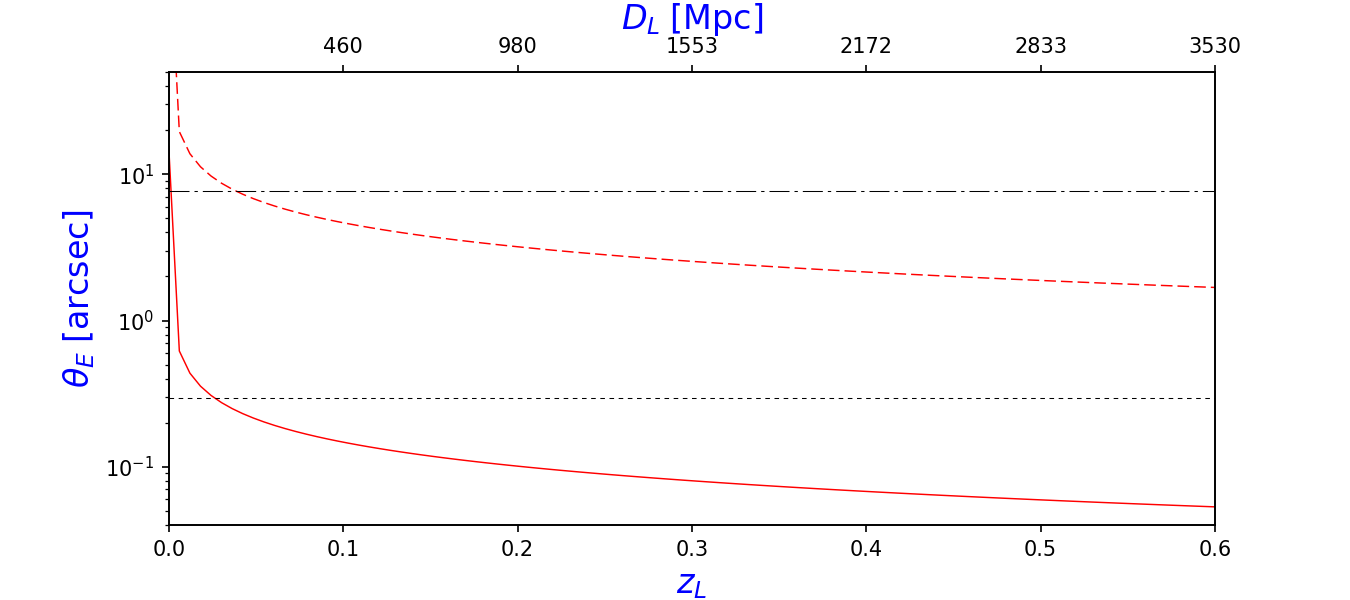
\includegraphics[scale=0.8]{5_HALOS/radio_einstein.png}
      \caption{\small Variación del radio de Einstein con la distancia observador-lente (Ecuación \ref{eq:radio_einstein_magnitud}) suponiendo un objeto lente puntual de masa \masassolares{10^9}(curva roja continua) y masa \masassolares{10^{12}}(curva roja discontinua). La lineas horizontales representan los limites de resolución de los catálogos \hatlas\ (\maths{{\sigma}_{h}^{p}\sim7.63\;\mathrm{arcsec}}) y \gama\  (\maths{{\sigma}_{g}^{p}\sim0.297\;\mathrm{arcsec})}. El intervalo \maths{z_L} cubre el rango de valores que toma el \rt\ para la gran mayoría de los objetos del catálogo \gama\ (ver Figura \ref{fig:histograma_z_gama}). La escala que aparece sobre la parte inferior de la figura es el \rt\ equivalente a la distancia que aparece en la escala superior de la figura según el modelo Lambda-CDM \footnotemark. Obsérvese que la Ecuación \ref{eq:radio_einstein_magnitud} relaciona \maths{\theta_E} con \maths{D_L}, no con \maths{z_L} que es lo que se mide directamente a partir de la observación del objeto.}
  \label{fig:radio_einstein}
  \end{center}
\end{figure}
\footnotetext{Para realizar este cálculo se ha utilizando el paquete \texttt{astropy.cosmology} y el modelo Lambda-CDM (Lambda Cold Dark Matter) con valor de la constante de Hubble 70 \maths{\mathrm{km\;{s}^{-1}\;{Mpc}^{-1} }} y densidad de la materia no relativista en unidades de la densidad crítica \maths{\Omega_{0}}=0.3.}

Nosotros no esperamos encontrar anillos de Einstein, pero los emparejados que estamos buscando forman lentes gravitatorias fuertes y sabemos que separación angular entre nuestros candidatos a lente gravitatoria debe ser de ese orden de magnitud. Teniendo en cuenta el radio efectivo de una galaxia elíptica de gran tamaño, su masa y un desplazamiento al rojo \maths{z\sim0.1}, cabria esperar una separación angular de \maths{\sim17\:\mathrm{arcsec}}. Dado que se trata de un caso extremo para una galaxia especialmente grande y especialmente próxima el resto de candidatos deben mostrar separaciones angulares inferiores.

La idea del método que proponemos es encontrar lentes gravitatorias en un subconjunto de emparejados que surgen al aplicar el método de \cross\ de catálogos de galaxias descrito en la sección anterior al considerar los catálogos \hatlas y \gama. Se trata de observaciones que dada su proximidad angular podrían pertenecer al mismo objeto, pero que sin embargo tienen \rts\ diferentes (esto es equivalente a decir que se cumplen las condiciones \maths{B^{p}_{12}>1} y \maths{B_{12}<1}).
Como hemos visto en la Sección~\ref{sec:4_cross_identificacion}, dada la resolución angular de los catálogos utilizados, el factor de Bayes posicional considerado toma el valor 1 cuando la separación angular de dos observaciones se encuentra en  \maths{\sim49.64\;\mathrm{arcsec}}. Esta distancia angular es varias veces mayor que la distancia de angular máxima que estimamos para la lente gravitatoria. Esto resulta beneficioso por una parte porque de esta manera probablemente la mayor parte de las lentes gravitatorias cuando intervienen dos objetos pertenezcan a este conjunto, pero también es un problema porque si la distancia de emparejamiento es muy grande, se incrementará también el número de contrapartidas formadas por observaciones entre objetos que no guardan ningún tipo de relación entre sí. Lo ideal sería que la distancia para la cuál \maths{B_{12}^{p}=1} se encontrase en \maths{\sim17\:\mathrm{arcsec}}.

A modo de resumen, el procedimiento que se va a seguir en este trabajo para identificar lentes gravitatorias será el siguiente: 

\vspace{-3mm}

\begin{itemize}
    
    \item Seleccionaremos todas aquellas observaciones de los catálogos \hatlas\ y \gama\ de los cuales disponemos una medida razonable de su \rt \footnote{Por medida razonable del \rt\ entendemos, una medida del \rt\ proporcionada por los catálogos o una estimación válida obtenida mediante el método descrito en la Sección~\ref{sec:3_redshift_hatlas}. Obsérvese este método solo sirve para galaxias lejanas en formación. Estos objetos son abundantes a \rts\ altos, pero no son los únicos. El método propuesto para la identificación de lentes gravitatorias no depende de si las fuentes son ETGs o no.}.
    
    \item Partiendo de la selección anterior, se realizará una búsqueda exhaustiva de todos las las observaciones del catálogo \hatlas\ DR1 que se encuentran a una distancia inferior a los \maths{\sim49.64\;\mathrm{arcsec}} de otro de \gama. En realidad, en este trabajo se ha escogido una distancia de emparejamiento de \maths{54\;\mathrm{arcsec}} y después se ha utilizado la condición de \maths{B^{p}_{12}<1}, pero esto es equivalente a elegir una distancia de emparejamiento de máxima de \maths{\sim49,64\;\mathrm{arcsec}} desde el principio.
    
    \item A cada emparejado, le asignaremos tres factores de Bayes: \maths{B^{p}_{12}}, \maths{B^{z}_{12}} y \maths{B_{12}}. Seleccionaremos aquellos que cumplen las condiciones de \maths{B^{p}_{12}>1} y \maths{B_{12}<1}.
    
    \item Por último seleccionaremos aquellos emparejados en los que \maths{z_{h}\!>\!1} (para poder considerar la observación perteneciente \hatlas\ un objeto con alto \rt ) y \maths{z_{h}>z_{g}} (ya que los objetos lente los buscamos en \gama\ y las fuentes en \hatlas ). La muestra resultante será nuestra selección de candidatos a sistemas lente gravitatoria en la que participa una fuente con un alto \rt.
    
\end{itemize}

\section{Resultados y análisis}\label{sec:6_resultados}

A continuación expondremos los resultados que hemos obtenido al aplicar los criterios de selección de candidatos a SLGs sobre las regiones seleccionadas.

\subsection{Candidatos según Negrello et al. y González-Nuevo et al. }\label{subsec:resultados_criterios_anteriores}

Nosotros hemos utilizado los criterios de \cite{article:Negrello_2010} y de \cite{article:Nuevo_2012} para identificar SLGs en el catálogo \hatlas\ DR1 y hemos encontrado que hay 20 objetos que cumplen el criterio de \cite{article:Negrello_2010}, 147 que cumplen el criterio de \cite{article:Nuevo_2012} y 10 que cumplen ambos criterios. Teniendo en cuenta que el catálogo cubre un área de \maths{\sim 161\:\mathrm{deg}^2} estimamos que hay una densidad de objetos de \maths{\sim 0.124\:\mathrm{deg}^{-2}} para aquellos que cumplen el primer criterio, de \maths{\sim 0.913\:\mathrm{deg}^{-2}} que cumplen el segundo y de \maths{\sim 0.975\:\mathrm{deg}^{-2}} si consideramos todos aquellos objetos que cumplen al menos uno de los criterios anteriores. 

Por tanto las densidades de objetos que cumplen estos criterios en el catálogo \hatlas\ DR1 son inferiores a las estimaciones previas que se habían realizado. Compárese la densidad de objetos que hemos encontrado, \maths{\sim0.1\:\mathrm{deg}^{-2}} y  \maths{\sim1\:\mathrm{deg}^{-2}} cuando las estimaciones eran \maths{\sim 0.3\:\mathrm{deg}^{-2}} y \maths{\sim 1.5-2\:\mathrm{deg}^{-2}} respectivamente \citep{article:Nuevo_2012}.

\subsection{Candidatos según el criterio bayesiano}\label{subsec:6_slgs_propuestos}

En la zona de intersección de los catálogos \hatlas\ DR1 y \gama\  se han encontrado 3824 contrapartidas que cumplen las condiciones para ser candidatos a sistema lente gravitatoria según el criterio bayesiano que hemos propuesto en la Sección~\ref{sec:5_halos}. Este conjunto contrapartidas se ha dividido en dos categorías. La primera formada por aquellas observaciones que disponían de \rt\ espectroscópico en ambos casos y la segunda formada por las observaciones pertenecientes al catálogo \hatlas\ que tienen un \rt\ obtenido mediante el procedimiento descrito en la Sección~\ref{sec:3_redshift_hatlas}. De la primera categoría se han encontrado 116 contrapartidas y de la segunda 3708. Entre las contrapartidas propuestos se han encontrado 16 en las cuales la observación de \hatlas\ cumple los criterios de \cite{article:Nuevo_2012} o \cite{article:Negrello_2010} para ser SLGs. 

Por otra parte también se ha realizado una simulación en la que a cada observación se le ha reasignado una posición aleatoria sobre una región con un área equivalente al área del catálogo al que pertenece. Después estas dos regiones se han solapado en un área igual al área de intersección de los catálogos originales y se ha procedido ha realizar un conteo de las contrapartidas exactamente de la misma forma que la que se ha llevado a cabo con las muestras originales. Esta simulación se ha repetido mil veces encontrándose \maths{3521\pm58} contrapartidas que cumplen los criterios para ser candidatas a sistema lente gravitatoria, de las cuales \maths{111\pm11} pertenecen a la primera categoría y \maths{3410\pm57} pertenecen a la segunda. Entre estos candidatos hay \maths{26\pm5} contrapartidas en las que además la observación en \hatlas\ cumple los criterios de \cite{article:Nuevo_2012} o \cite{article:Negrello_2010}.

Estos resultados indican que hay \maths{\sim200-300} contrapartidas que no pueden ser explicadas por una distribución aleatoria de las observaciones, sin embargo, evidencian también que nuestra muestra tiene un número muy elevado de contrapartidas formadas por observaciones que no tienen ninguna relación entre sí. 

La mayor diferencia entre la muestra simulada y la real se encuentra entre los objetos de la segunda categoría con una diferencia de un \maths{8\%} de la muestra real. También es significativo que en la muestra simulada se estén encontrando más contrapartidas en las que se cumplen los criterios de \cite{article:Nuevo_2012} o \cite{article:Negrello_2010} que para el caso de la muestra real. Esto nos está indicando que los objetos seleccionados por nuestro criterio de identificación\linebreak son diferentes a los seleccionados por estos dos criterios para la identificación de SLGs.

\begin{figure}[ht]
\captionsetup[subfigure]{labelformat=empty}
  \begin{center} 
  
    \subfloat[]{
     \label{subfig:log_bayes_ajuste}
      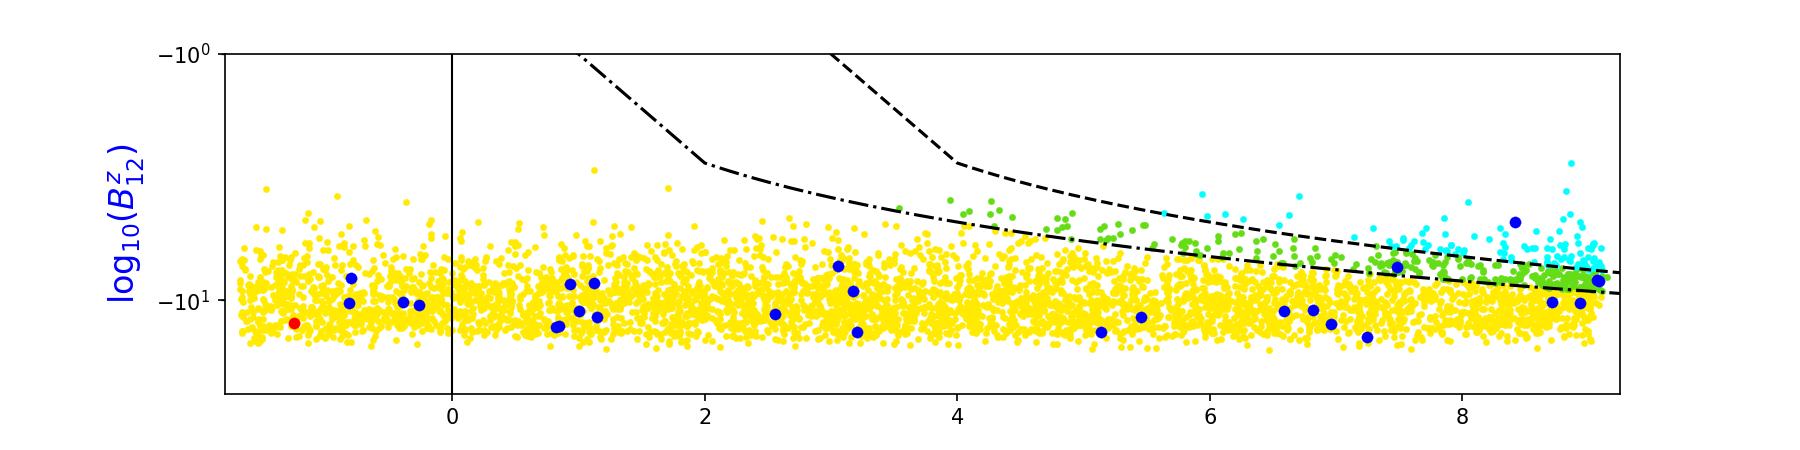
\includegraphics[width=\textwidth]{6_Resultados/matching_ghfactor_bayes_log_semilog_ajuste.png}}
      \vspace*{-23mm}
      
    \subfloat[]{
     \label{subfig:log_bayes_todos}
      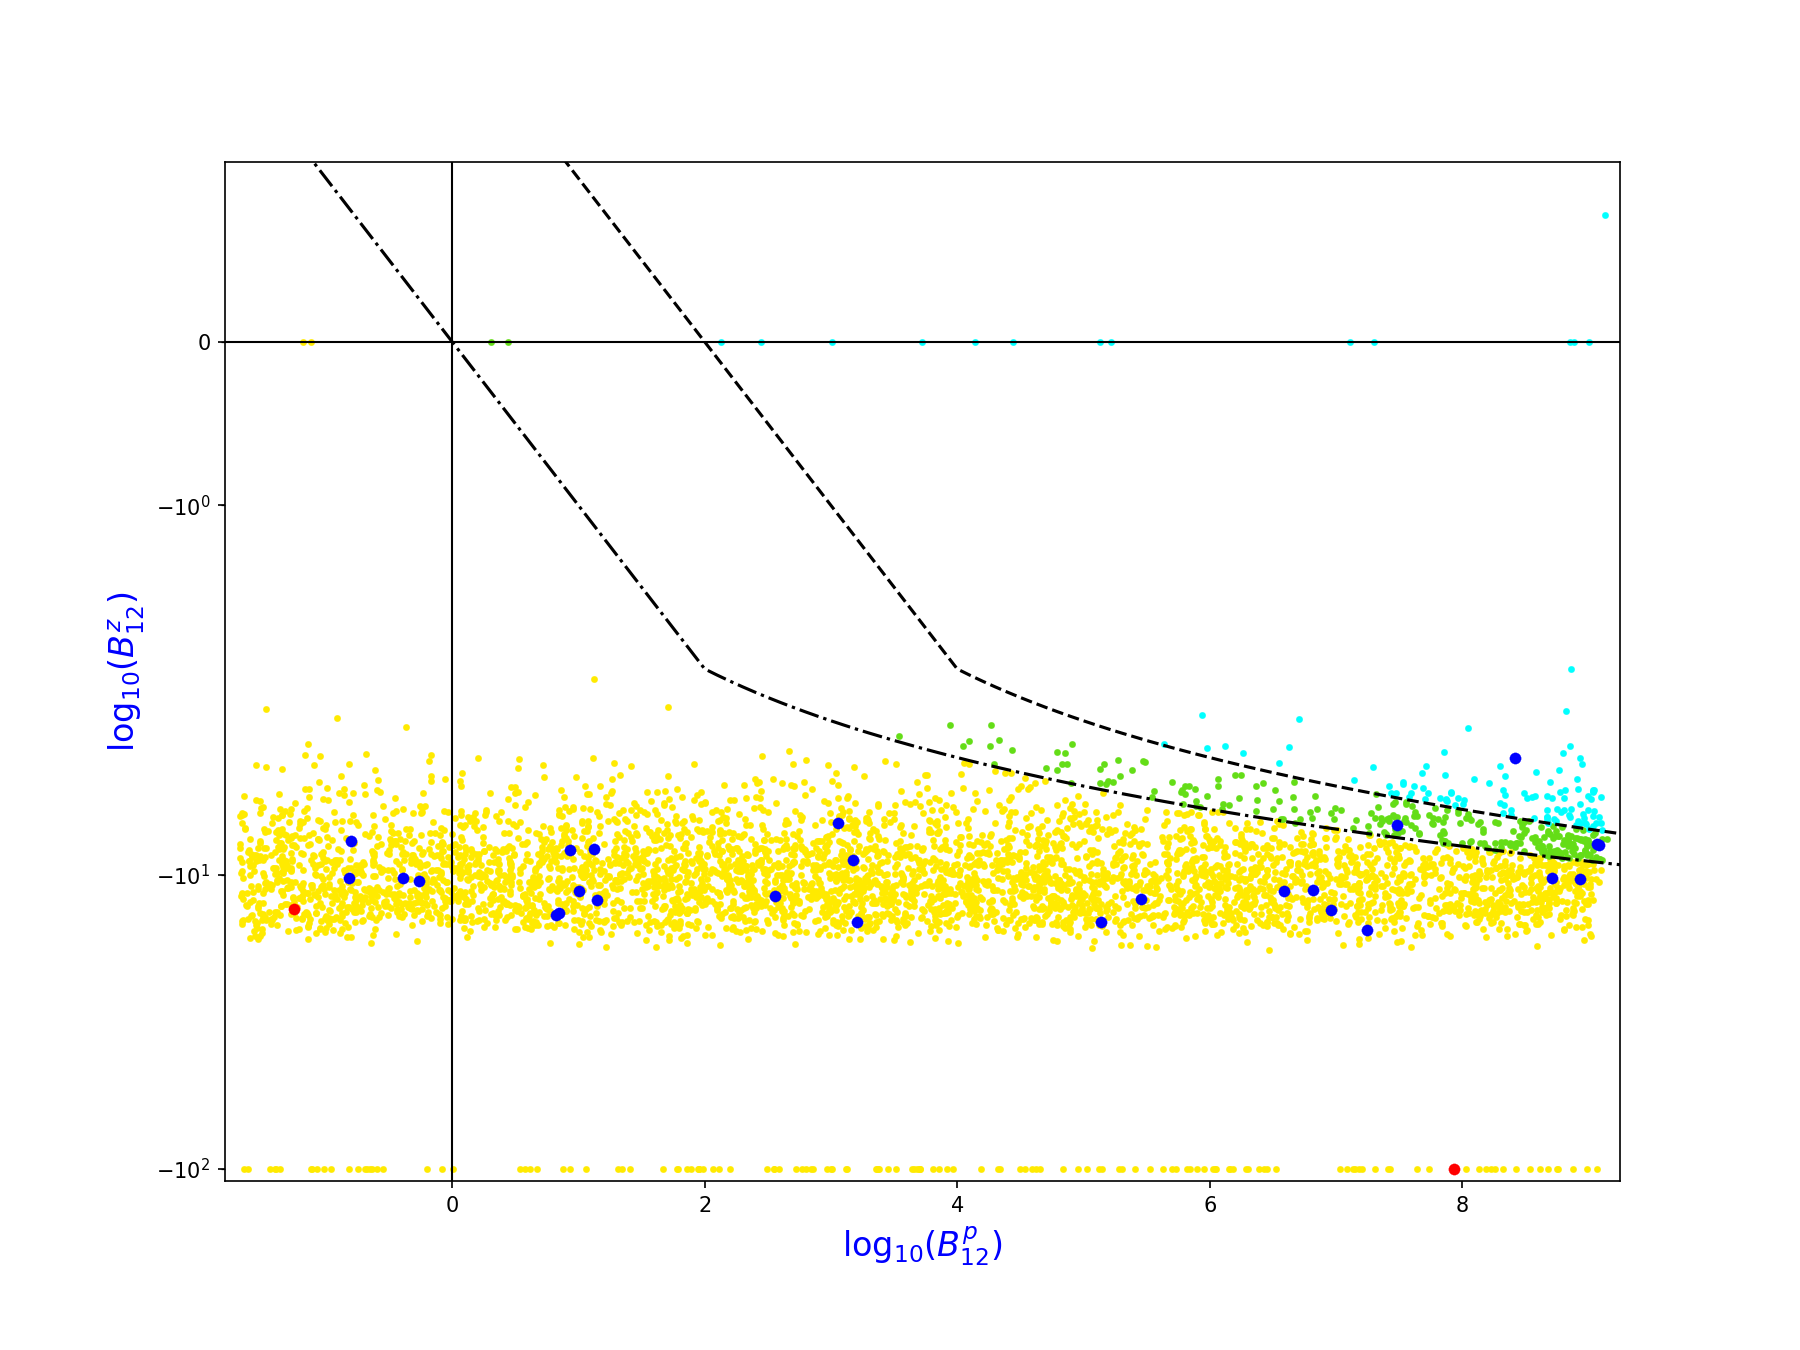
\includegraphics[width=\textwidth]{6_Resultados/matching_ghfactor_bayes_log_semilog.png}}
      
  \end{center}
  \vspace*{-20mm}
  \caption{\small Representación del logaritmo en base diez del factor de Bayes espectroscópico, \maths{B^{z}_{12}} (en la figura, el logaritmo está en escala logarítmica) frente al logaritmo en base diez del factor de Bayes posicional, \maths{B^{p}_{12}} para un total de 4938 emparejamientos que cumplen que \maths{z_{h}\;>\,1}, \maths{z_{h}>z_{g}} y \maths{\phi<54\;\mathrm{arcsec}}. Los puntos de color rojo son los pareados en los que participa un candidato a \halo\ que cumple el criterio de \cite{article:Negrello_2010}; en los de color azul añil participa un candidato a \halo\ que no cumple la condición anterior, pero si que cumple el criterio de \cite{article:Nuevo_2012}; los de color azul cian, son aquellos que no cumplen ninguno de los criterios anteriores pero tienen un  valor \maths{B_{12}>100} (la confianza sobre la hipótesis de que se trata del mismo objeto es absoluta); los de color verde no cumplen ninguno de los criterios anteriores pero \maths{1>B_{12}>100}; el resto de pareados se representan de color anaranjado. Dado que \maths{\log_{10}(0)=-\infty}, cuando se cumple la condición de que el pareado tiene un valor \maths{B^{z}_{12}<{10}^{-100}} entonces se le reasigna el valor  \maths{B^{z}_{12}={10}^{-100}}. La línea vertical continua divide la figura en dos secciones, con \maths{B^{p}_{12}<1} y \maths{B^{p}_{12}>1}. Los puntos con \maths{B^{p}_{12}<1} se corresponden con aquellas contrapartidas con una separación angular \maths{\phi\geqslant49.64\:\mathrm{arcsec}}. En la zona superior de la figura, se han destacado aquellos pareados en los que participan objetos de \hatlas\ cuyo redshift ha sido calculado mediante el método descrito en la Sección~\ref{sec:3_redshift_hatlas}. Los candidatos propuestos por nuestro criterio están representados en la zona con \maths{B^{p}_{12}>1} y \maths{B_{12}<1}.}
  \label{fig:log_bayes}
\end{figure}

\section{Discusión y conclusiones}\label{sec:7_conclusiones}

Para considerar que nuestro método supone un método fiable para la identificación de sistemas lente gravitatoria, el número de contrapartidas que no pueden ser explicadas por una distribución aleatoria debería ser mucho mayor que el número de asociaciones aleatorias que cumplen nuestros criterios y lo que encontramos es justo lo contrario. Los resultados de la simulación indican que siempre que tengamos una población de observaciones con una densidad como la que tenemos en la muestra, es inevitable que se formen del orden de \maths{\sim3500} emparejamientos entre observaciones que distan a \maths{\lesssim50\:\mathrm{arcsec}} que no tienen ningún tipo de interacción física. Si las medidas que caracterizan a cada observación fuesen más precisas y más exactas se haría evidente que muchos de los candidatos propuestos o bien se encuentran a una distancia demasiado grande para ser considerados candidatos a lente o bien son observaciones de un mismo objeto en los dos catálogos.

La gran mayoría de los desplazamientos al rojo pertenecientes a las observaciones de \hatlas\ que participan en el pareo (\anglicismo{matching}) han sido determinados mediante el ajuste de la SED de la galaxia \smm. Como hemos visto en la Sección~\ref{sec:3_redshift_hatlas} tenemos cierta confianza de que el ajuste es válido para estimar el \rt\ de las galaxias en formación, pero no sabemos cuantas de las observaciones de las que hemos estimado el \rt\ son en realidad observaciones de galaxias lejanas. Es posible que estemos realizando un ajuste a galaxias que en realidad se encuentran mucho más cerca. De hecho se podría explicar que encontremos más contrapartidas en la muestra real que en la simulada sin que se diera el fenómeno de lente gravitatoria; ese exceso de contrapartidas podría deberse a observaciones del mismo objeto en los dos catálogos que no hemos sido capaces de identificar como tal porque nuestra estimación del \rt\ es incorrecta.

En este trabajo hemos utilizado el método descrito en la Sección~\ref{sec:3_redshift_hatlas} para estimar el \rt\ de muchos de los objetos del catálogo \hatlas. Para considerar válida esta medida del ajuste debían cumplirse varias condiciones: no haber una estimación previa del corrimiento al rojo de esa observación, debe ser una galaxia (recordemos, según la información disponible en columna GSQ\_FLAG de este mismo catálogo) y el valor del ajuste debe encontrarse en un rango comprendido entre \maths{z=1} y \maths{z=3.5}. Opino que deberíamos buscar más indicios antes de considerar válido el ajuste realizado con ese método. 

Nuestra propuesta para identificar lentes gravitatorias se ha planteado en el supuesto de que únicamente interviene un único objeto como lente, sin embargo, en muchas ocasiones intervienen grupos de galaxias y no galaxias individuales en constitución de la lente. El criterio de que se trata de una lente gravitatoria por el hecho encontrar dos objetos con \rt\ diferentes suficientemente próximos posiblemente también sea poco realista. Partiendo de un estudio cuidadoso del entorno que se encuentran lentes gravitatorias confirmadas podríamos elaborar métodos para la identificación de entornos favorables para la presencia de lentes gravitatorias. En este sentido es posible que tengamos que identificar cúmulos de galaxias más que objetos individuales como lentes gravitatorias.

El criterio Bayesiano descrito en la Sección~\ref{sec:4_cross_identificacion} es un criterio de \cross\ de catálogos y por tanto no ha sido pensado para la identificación SLGs. Los factores bayesianos están diseñados para contrastar la hipótesis \maths{H_1} que supone los emparejados están formados por observaciones de un mismo objeto astronómico frente a la hipótesis \maths{H_2} que supone que las observaciones pertenecen a dos objetos diferentes. Deberían plantearse nuevos factores de Bayes, que permitieran contrastar por ejemplo la hipótesis de que una observación considerada pertenece a una ETGs o no, o la hipótesis de que el emparejado considerado es una lente gravitatoria frente a la hipótesis de que no lo es. Plantear estos factores de Bayes exige conocer con mayor profundidad el fenómeno de las lentes gravitatorias y la naturaleza de las ETGs, lo cual se escapa los objetivos académicos de este trabajo.

También hay lugar para mejorar nuestro método de \cross. Los factores de Bayes son quizás demasiado simples y se pueden mejorar. Las funciones densidad de \cultismo{probabilidad a priori} son funciones no informativas que se han introducido por simplicidad matemática pero cabe plantearse otras más adecuadas. Por ejemplo podríamos incorporar la información de la que disponemos sobre la distribución del \rt\ en los catálogos para mejorar el factor de Bayes fotométrico. El modelo de precisión astrométrica que se ha considerado es bastante conservador. Se ha considerado que el error astrométrico es igual a la resolución angular del telescopio, lo cuál es razonable cuando las fuentes son puntuales. Las galaxias que aparecen el los catálogos no son puntuales, tienen una extensión y en estos casos es frecuente que \maths{\sigma^p} sea inferior a la resolución angular del telescopio. Se podría haber tomado un valor de \maths{\sigma^p} menor, pero no se ha hecho por prudencia.

La resolución espacial del telescopio \h\ también juega un papel fundamental en este trabajo. Una mejora de este parámetro permitiría tener unas medidas sobre el flujo de las fuentes más precisas con una menor contaminación por parte de las fuentes próximas más débiles. Además permitiría mejorar los modelos de la SED de las galaxias tempranas y podríamos introducir mejoras en nuestro método para la estimación del \rt\ fotométrico. No solo eso. La mejora del modelo de precisión astrométrica, junto con una menor incertidumbre asociada a la posición de la fuente permitiría estudiar las estructuras formadas por las lentes gravitatorias a una escala menor, más adecuada al orden de magnitud en el que se producen estos fenómenos. Esto también reduciría la distancia máxima de emparejamiento que se ha considerado entre las fuentes y se producirían menos emparejamientos aleatorios entre observaciones de objetos que no guardan ningún tipo de relación entre sí.

Por tanto no podemos considerar nuestro método como una alternativa razonable a las ya existentes y tampoco tiene mucho sentido comparar el número de candidatos obtenidos por nuestro método con el número obtenido utilizando los métodos que encontramos en la literatura. Sin embargo se pueden plantear modificaciones en el método que quizás conduzcan a una selección de candidatos más fiable y con mayor pureza. Además podríamos considerar el método propuesto como una fase previa a un estudio más detallado porque permitiría identificar de una forma rápida, sencilla y directa, basada en un criterio estadístico riguroso, en torno al tres por ciento de los candidatos con mayor probabilidad de ser sistemas lente de entre las galaxias del catálogo \hatlas\ DR1.

\appendix

\section{Redshifts fotométricos de los candidatos }\label{apendice:tab:articulo}

\begin{table}[!ht]
\centering
\pgfplotstabletypeset[
    col sep=comma,
    columns={HATLASDR1,RA,DEC,S500,eS500,S350,eS350,S250,eS250,ZA,ErrorZA,ZB,ErrorZB},
    brackets/.style={
        postproc cell content/.append style={/pgfplots/table/@cell content/.add={\relax[}{]}},
    },
    parenthesis/.style={
        postproc cell content/.append style={/pgfplots/table/@cell content/.add={\relax(}{)}},
    },
    display columns/0/.style={
        string type,
        column name={$\qquad$H-ATLAS},
        column type={l}
    },
    display columns/1/.style={
        column name={RA},
        fixed,
        zerofill,
        precision=3,
    },
    columns/2/.style={
        column name={DEC},
        fixed,
        zerofill,
        precision=4,
    },
    display columns/3/.style={
        column name={$S_{500}\,$},
        fixed,
        zerofill,
        precision=0,
        column type/.add={}{@{\hspace{0mm}}}
    },
    display columns/4/.style={
        column name={\scriptsize{(mJy)}},
        fixed,
        zerofill,
        precision=0,
        parenthesis
    },
    display columns/5/.style={
        column name={$S_{350}\,$},
        fixed,
        zerofill,
        precision=0,
        column type/.add={}{@{\hspace{0mm}}}
    },
    display columns/6/.style={
        column name={\scriptsize{(mJy)}},
        fixed,
        zerofill,
        precision=0,
        parenthesis
    },
    display columns/7/.style={
        column name={$S_{250}\,$},
        fixed,
        zerofill,
        precision=0,
        column type/.add={}{@{\hspace{0mm}}}
    },
    display columns/8/.style={
        column name={\scriptsize{(mJy)}},
        fixed,
        zerofill,
        precision=0,
        parenthesis
    },
    display columns/9/.style={
        column name={$\;\;{z}_{\mathrm{H}}$},
        fixed,
        zerofill,
        precision=2,
        column type/.add={}{@{\hspace{1mm}}}
    },
    display columns/10/.style={
        column name={${\sigma}_{\mathrm{H}}$},
        fixed,
        zerofill,
        precision=2,
        parenthesis
    },
    display columns/11/.style={
        column name={$\;\;{z}_{\mathrm{phot}}$ },
        fixed,
        zerofill,
        precision=2,
        column type/.add={}{@{\hspace{1mm}}}
    },
    display columns/12/.style={
        column name={${\sigma}_{\mathrm{phot}}$},
        fixed,
        zerofill,
        precision=2,
        parenthesis
    },
    font=\footnotesize,
    every head row/.style={before row=\toprule,after row=\midrule},
    every last row/.style={after row=\bottomrule}
]{Apendices/a_tb64/comparacion_z.csv}
\end{table}


% \newgeometry{top=15mm, bottom=2.5mm}

\begin{table}[!ht]
\centering
\pgfplotstabletypeset[
    col sep=comma,
    columns={HATLASDR1,RA,DEC,S500,eS500,S350,eS350,S250,eS250,ZA,ErrorZA,ZB,ErrorZB},
    brackets/.style={
        postproc cell content/.append style={/pgfplots/table/@cell content/.add={\relax[}{]}},
    },
    parenthesis/.style={
        postproc cell content/.append style={/pgfplots/table/@cell content/.add={\relax(}{)}},
    },
    display columns/0/.style={
        string type,
        column name={$\qquad$H-ATLAS},
        column type={l}%lo alinea a la iz
    },
    display columns/1/.style={
        column name={RA},
        fixed,
        zerofill,
        precision=3,
        fonts by sign={}{\color{red}},
    },
    columns/2/.style={
        column name={DEC},
        fixed,
        zerofill,
        precision=4,
    },
    display columns/3/.style={
        column name={$S_{500}\,$},
        fixed,
        zerofill,
        precision=0,
        column type/.add={}{@{\hspace{0mm}}}
    },
    display columns/4/.style={
        column name={\scriptsize{(mJy)}},
        fixed,
        zerofill,
        precision=0,
        parenthesis
    },
    display columns/5/.style={
        column name={$S_{350}\,$},
        fixed,
        zerofill,
        precision=0,
        column type/.add={}{@{\hspace{0mm}}}
    },
    display columns/6/.style={
        column name={\scriptsize{(mJy)}},
        fixed,
        zerofill,
        precision=0,
        parenthesis
    },
    display columns/7/.style={
        column name={$S_{250}\,$},
        fixed,
        zerofill,
        precision=0,
        column type/.add={}{@{\hspace{0mm}}}
    },
    display columns/8/.style={
        column name={\scriptsize{(mJy)}},
        fixed,
        zerofill,
        precision=0,
        parenthesis
    },
    display columns/9/.style={
        column name={$\;\,{z}_{\mathrm{H}}$},
        fixed,
        zerofill,
        precision=2,
        column type/.add={}{@{\hspace{1mm}}}
    },
    display columns/10/.style={
        column name={${\sigma}_{\mathrm{H}}$},
        fixed,
        zerofill,
        precision=2,
        parenthesis
    },
    display columns/11/.style={
        column name={$\;\;{z}_{\mathrm{phot}}$ },
        fixed,
        zerofill,
        precision=2,
        column type/.add={}{@{\hspace{1mm}}}
    },
    display columns/12/.style={
        column name={${\sigma}_{\mathrm{phot}}$},
        fixed,
        zerofill,
        precision=2,
        parenthesis
    },
    font=\footnotesize,
    every head row/.style={before row=\toprule,after row=\midrule},
    every last row/.style={after row=\bottomrule}
]{Apendices/a_tb64/comparacion_z2.csv}
\caption{Muestra de 64 candidatos a SLGs procedente del articulo \cite{article:Nuevo_2012}. Los errores se encuentran entre paréntesis a la derecha de cada medida. La columna \maths{z_{\mathrm{H}}} contiene los valores del \rt\ que estos autores proponen para estos objetos mientras que la columna \maths{z} contiene los valores obtenidos a partir de nuestro código.}
\label{tab:redshift_halos}
\end{table}


\section{Selección de objetos del catálogo GAMA }\label{apendice:tab:sigmas}

\begin{table}[!ht]
\centering
\pgfplotstabletypeset[
    col sep=comma,
    columns={n,id,zg,zn,szn,source,quality},
    brackets/.style={
        postproc cell content/.append style={/pgfplots/table/@cell content/.add={\relax[}{]}},
    },
    parenthesis/.style={
        postproc cell content/.append style={/pgfplots/table/@cell content/.add={\relax(}{)}},
    },
    display columns/0/.style={
        column name={N},
        fixed,
        zerofill,
        precision=0,
        column type={l}%lo alinea a la iz
    },
    display columns/1/.style={
        column name={GAMA\_IAU\_ID},
        string type,
        column type={l}%lo alinea a la iz
    },
    display columns/2/.style={
        column name={Z\_HELIO},
        fixed,
        zerofill,
        precision=6,
    },
    display columns/3/.style={
        column name={z (NED)},
        fixed,
        zerofill,
        precision=6,
    },
    display columns/4/.style={
        column name={${\sigma}^{z}$ (NED)},
        fixed,
        zerofill,
        precision=6,
    },
    display columns/5/.style={
        column name={Z\_SOURCE},
        fixed,
        zerofill,
        precision=0,
    },
    display columns/6/.style={
        column name={Z\_QUALITY},
        fixed,
        zerofill,
        precision=0,
    },
    font=\footnotesize,
    every head row/.style={before row=\toprule,after row=\midrule},
    every last row/.style={after row=\bottomrule}
]{Apendices/b_tbSIGMAGAMA/gama_redshift_tabla.csv}
\caption{Muestra que contiene 27 observaciones procedentes del catálogo \gama\ DR1 cuyo \rt\ se encuentra también disponible en la base de datos NED.}
\label{tab:ajuste_error_gama}
\end{table}

\section{Selección de objetos del catálogo GAMA }\label{apendice:tab:sigmas}

\begin{table}[!ht]
\centering
\pgfplotstabletypeset[
    col sep=comma,
    columns={n,id,zg,zn,szn,source,quality},
    brackets/.style={
        postproc cell content/.append style={/pgfplots/table/@cell content/.add={\relax[}{]}},
    },
    parenthesis/.style={
        postproc cell content/.append style={/pgfplots/table/@cell content/.add={\relax(}{)}},
    },
    display columns/0/.style={
        column name={N},
        fixed,
        zerofill,
        precision=0,
        column type={l}%lo alinea a la iz
    },
    display columns/1/.style={
        column name={GAMA\_IAU\_ID},
        string type,
        column type={l}%lo alinea a la iz
    },
    display columns/2/.style={
        column name={Z\_HELIO},
        fixed,
        zerofill,
        precision=6,
    },
    display columns/3/.style={
        column name={z (NED)},
        fixed,
        zerofill,
        precision=6,
    },
    display columns/4/.style={
        column name={${\sigma}_{z}$ (NED)},
        fixed,
        zerofill,
        precision=6,
    },
    display columns/5/.style={
        column name={Z\_SOURCE},
        fixed,
        zerofill,
        precision=0,
    },
    display columns/6/.style={
        column name={Z\_QUALITY},
        fixed,
        zerofill,
        precision=0,
    },
    font=\footnotesize,
    every head row/.style={before row=\toprule,after row=\midrule},
    every last row/.style={after row=\bottomrule}
]{Apendices/b_tbSIGMAGAMA/gama_redshift_tabla.csv}
\caption{Muestra que contiene 27 observaciones procedentes del catálogo \gama\ DR1 cuyo \rt\ se encuentra también disponible en la base de datos NED.}
\label{tab:ajuste_error_gama}
\end{table}

\section{Código en \texttt{Python}}\label{apendice:tb_codigo}

Los programas que se presentan en esta sección contienen todo lo necesario para realizar todos los cálculos y gráficas a los que se ha hecho referencia en las secciones anteriores; están escritos en lenguaje de programación \texttt{Python 3.6.0} y se requiere tener instaladas las librerías \texttt{scipy 0.18}, \texttt{matplotlib 2.0.0}, \texttt{numpy 1.11.3} y \texttt{astropy 1.3}.
El código se encuentra repartido en varios ficheros llamados módulos. Para que los ejecutables funcionen correctamente, sin cambiar nada, debemos mantener la siguiente estructura de directorios: 

\hspace{3mm}

\begin{tikzpicture}[
    scale=.7,
    grow via three points={one child at (0.5,-0.65) and
    two children at (0.5,-0.65) and (0.5,-1.1)},
    edge from parent path={(\tikzparentnode.south) |- (\tikzchildnode.west)}]
  \node [root] {dir}
    child { node [selected] {packages}
        child { node {factor\_bayes.py}}
        child { node {get.py}}
        child { node {rojo.py}}
    }
    child { node at (0,-2)[selected] {p1\_halos}
        child { node [selected] {inroute}
            child { node {tabla\_Gonzalez-Nuevo\_2012.fits}}
            child { node {SMM\_template\_norm.sed}}
        }
        child { node at (0,-1.3)[selected] {outroute}}
        child { node at (0,-1.4){main\_halos.py}}
    }       
    child { node at (13,-1)[selected] {p2\_matching}
        child { node [selected] {inroute}
            child { node {GamaCoreDR1\_v1.fits}}
            child { node { HATLAS\_DR1\_CATALOGUE\_V1.2.FITS}}
            child { node { nombres\_candidatos.txt}}
            child { node { SMM\_template\_norm.sed}}
        }
        child { node at (0,-2.4)[selected] {outroute\_gama}}
        child { node at (0,-2.5)[selected] {outroute\_hatlas}}
        child { node at (0,-2.6)[selected] {outroute\_matching}}
        child { node at (0,-2.7){main\_gama.py}}
        child { node at (0,-2.8){main\_hatlas.py}}
        child { node at (0,-2.9){main\_matching\_gh.py}}
        child { node at (0,-3){main\_matching\_gh\_simulacion.py}}
    }
    child { node at (0,-5.1)[selected] {figuras\_adicionales}
        child { node [selected] {inroute}
            child { node {SMM\_template\_norm.sed}}
        }
        child { node at (0,-0.7)[selected] {outroute}}
        child { node at (0,-0.8){main\_ajuste\_error\_espec.py}}
        child { node at (0,-0.9){main\_radio\_Einstein\_D\_L.py}}
        child { node at (0,-1){main\_smm.py}}
    };
\end{tikzpicture}

\hspace{3mm}

Los ejecutables son todos aquellos ficheros cuyo nombre contiene la palabra \texttt{main}. Todos ellos leen los datos que necesitan de los ficheros situados en los directorios \texttt{inroute}, a excepción de los ejecutables \texttt{main\_matching.py} y \texttt{main\_matching\_simulacion.py} cuyos ficheros de entrada se encuentran en \texttt{outroute\_gama} y \texttt{outroute\_hatlas}. Las gráficas y tablas de datos se guardan en los directorios que contienen la palabra \texttt{outroute}. 

Todos los ejecutables hacen llamadas a una serie de funciones que son comunes, por ese motivo, para evitar repetir el código de esas funciones en cada ejecutable, éstas funciones se han definido en tres módulos que se encuentran el directorio \texttt{packages}. Cada módulo y cada función se encuentra debidamente comentada. Recuerdo al lector las cadenas de documentación son accesibles mediante:

\vspace{-2mm}

\begin{minted}{python}
    >>> help("nombre_modulo.nombre_funcion")
\end{minted}

\vspace{-4mm}

o

\vspace{-4mm}

\begin{minted}{python}
    >>> print(nombre_funcion.__doc__)
\end{minted}

\vspace{-2mm}

También se ha realizado un esquema sobre la estructura del ejecutable \texttt{main\_halos.py} (\ref{apendice:esquema_main_halos}). 

\let\thefootnote\relax\footnotetext{El código fuente de los programas escritos en \texttt{Python} y el escrito en \LaTeX\ con el que se obtiene este documento, están bajo licencia GPL.}

\newpage

\subsection{Esquema del módulo \texttt{main\_halos.py}}\label{apendice:esquema_main_halos}

\begin{figure}[!htp]
    \begin{center}
         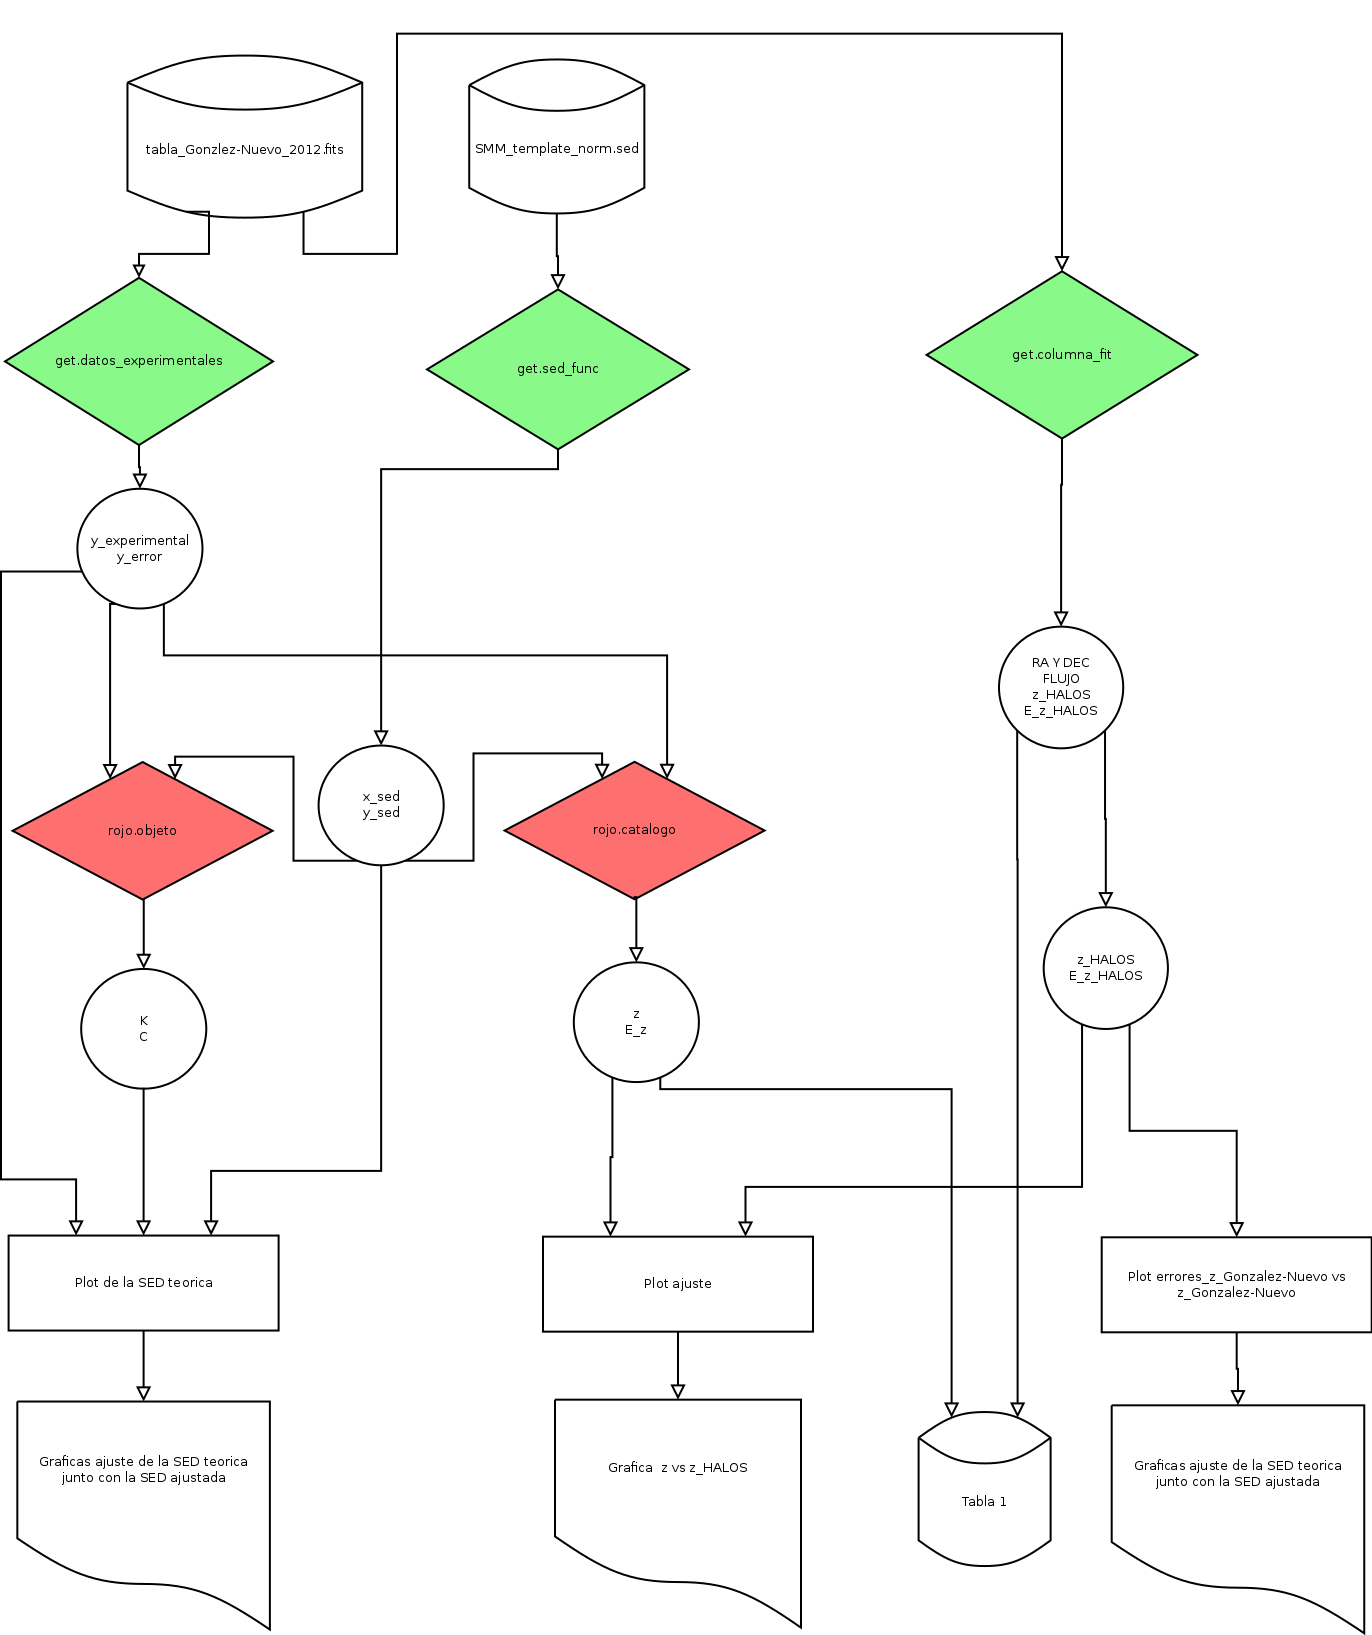
\includegraphics[width=16cm]{Apendices/codigo/Diagrama_p1.png}
    \end{center}
    \vspace{-3mm}
    \caption{Este esquema representa la estructura completa del ejecutable \texttt{main\_halos.py}. Los ficheros con formato \texttt{.fits} están representados mediante figuras cilíndricas; los que se encuentran en la parte superior de la figura, son los ficheros de entrada y el situado en la parte inferior es el fichero de salida a partir del cual se obtiene la tabla \ref{tab:redshift_halos}. Este ejecutable también devuelve varias figuras representadas en la zona inferior del esquema. Las funciones se representan mediante rombos y los colores ayudan a identificar el módulo en el que están definidas. La salida de que se obtiene a partir de cada función se encuentra en el interior de un círculo. }  
    \label{diagrama_flujo_main_halos}
\end{figure}

\newpage


\subsection{Módulo \texttt{main\_halos.py}}\label{apendice:codigo:main_halos}

\inputminted{python}{Apendices/codigo/main_halos.py}


\subsection{Módulo \texttt{main\_gama.py}}\label{apendice:codigo:main_gama}

\inputminted{python}{Apendices/codigo/main_gama.py}


\subsection{Módulo \texttt{main\_hatlas.py}}\label{apendice:codigo:main_hatlas}

\inputminted{python}{Apendices/codigo/main_hatlas.py}


\subsection{Módulo \texttt{main\_matching\_gh.py}}\label{apendice:codigo:main_matching_gh}

\inputminted{python}{Apendices/codigo/main_matching_gh.py}


\subsection{Módulo \texttt{main\_matching\_gh\_simulacion.py}}\label{apendice:codigo:main_matching_gh_simulacion}

\inputminted{python}{Apendices/codigo/main_matching_gh_simulacion.py}


\subsection{Módulo \texttt{factor\_bayes.py}}\label{apendice:codigo:factor_bayes}

\inputminted{python}{Apendices/codigo/factor_bayes.py}


\subsection{Módulo \texttt{rojo.py}}\label{apendice:codigo:rojo}

\inputminted{python}{Apendices/codigo/rojo.py}


\subsection{Módulo \texttt{get.py}}\label{apendice:codigo:get}

\inputminted{python}{Apendices/codigo/get.py}


\subsection{Módulo \texttt{main\_smm.py}}\label{apendice:codigo:main_smm}

\inputminted{python}{Apendices/codigo/main_smm.py}


\subsection{Módulo \texttt{main\_main\_radio\_Einstein\_D\_L.py}}\label{apendice:codigo:main_radio_Einstein_D_L}

\inputminted{python}{Apendices/codigo/main_radio_Einstein_D_L.py}


\subsection{Módulo \texttt{main\_ajuste\_error\_espec.py}}\label{apendice:codigo:main_ajuste_error_espec}

\inputminted{python}{Apendices/codigo/main_ajuste_error_espec.py}

%   Bibliografia
\bibliography{references}

\end{document}